% \newcommand{\yao}{垚} % 定义快捷命令，后续直接用\yao即可
% \documentclass[master,phil,fulltime,electronic,cenhdr,normaltoc,blind]{buptthesis} % 学硕电子版
%\documentclass[master,phil,fulltime,print,cenhdr,normaltoc]{buptthesis} % 学硕印刷版
\documentclass[master,eng,fulltime,electronic,cenhdr,normaltoc]{buptthesis} % 专硕电子版
%\documentclass[master,eng,fulltime,print,cenhdr,normaltoc]{buptthesis} % 专硕印刷版
%\documentclass[phd,phil,fulltime,electronic,cenhdr,normaltoc]{buptthesis} % 学博电子版
%\documentclass[phd,phil,fulltime,print,cenhdr,normaltoc]{buptthesis} % 学博印刷版
%\documentclass[phd,eng,fulltime,electronic,cenhdr,normaltoc]{buptthesis} % 专博电子版
%\documentclass[phd,eng,fulltime,print,cenhdr,normaltoc]{buptthesis} % 专博印刷版

% !UPDATE 20231210: add to remove `normaltoc` to remove table content in the toc

% 电子版和印刷版的区别
% 1. 电子版是没有跳偶数页，所有内容都是直接连起来的
% 2. 印刷版部分内容跳偶数页开头的，生成的PDF直接双页打印即可

% 盲审版在选项后加入`blind`，比如学硕电子版的盲审版指令如下：
% \documentclass[master,phil,fulltime,electronic,cenhdr,normaltoc,blind]{buptthesis} % 学硕电子版

\makeatletter
% 检查是否为盲审版本
\newif\ifWithOptionBlind 
\@ifclasswith{buptthesis}{blind}{\WithOptionBlindtrue}{\WithOptionBlindfalse}
% \newCJKfontfamily\RareCJK{FandolSong-Regular}
% \newcommand{\yao}{{\RareCJK 垚}}
\makeatother

% 导入宏包
\usepackage{graphicx}
\usepackage{bbding}
\usepackage{booktabs}
\usepackage{bicaption}
\usepackage{float}
\usepackage{gbt7714}
\usepackage{fontspec}
\usepackage{subcaption}
% 导言区必须加载的宏包（确保公式环境正常）
\usepackage{amsmath}  % 核心：支持equation/align等编号公式环境
\usepackage{amssymb}  % 可选：提供勒让德多项式等数学符号
\usepackage{ragged2e}
% \usepackage{xeCJK}
% \setCJKmainfont{SimSun} % Windows: SimSun；mac: Songti SC；Linux: Noto Serif CJK SC
% \usepackage{xeCJK}
% \setCJKmainfont{SimSun} % Windows: SimSun；mac: Songti SC；Linux: Noto Serif CJK SC
% --- 生僻字“垚”兜底字体（Overleaf 自带 Fandol 字体，稳定可用）---
% \newfontfamily\rareFont{resources/SourceHanSerifSC-Regular.otf}
% \newcommand{\yao}{{\rareFont 垚}}

% 定义使用的函数/宏
\DeclareMathOperator{\Tr}{Tr}


% 正文当中的其他定义
% \setmainfont{Times New Roman} % 英文字体使用Times New Roman
% \setmathfont{XITS Math} % 数学公式字体使用XITS Math

% 新增：配置支持生僻字的中文字体
% \setCJKmainfont{SimSun} % Windows自带宋体（支持垚、淼等生僻字）

\BUPTthesiscntitlepage{%
	confidential = {公开}, % 目前只支持公开
	title = {面向三维光场显示的人脸光照编辑方法研究},  % 本章标题
	studentid = {2023140412}, % 学号
	name = {杨\yao 杰}, % 姓名
	major = {新一代电子信息科学与技术(含量子技术等)}, % 专业名称
	supervisor = {桑新柱}, % 导师姓名
	institute = {电子工程学院} % 单行学院的写法
	%institute = {你的学院1\\你的学院2} % 双行学院的写法
}

%% \quad 相当于一个汉字的宽度，同时也相当于~~~~

% \BUPTdateOptions{%
%     pageYear = {2026}, % 封面上面的年
%     pageMonth = {2}, % 封面上面的月
%     pageDay = {20}, % 封面上面的天
%     dissertationYear = {2026}, % 答辩时间的年
%     dissertationMonth = {2}, % 答辩时间的月
%     dissertationDay = {20} % 答辩时间的天
% }

\BUPTthesisentitlepage{% 
	confidentialEN = {Public},  % 目前只支持公开
	titleEN = {Research on Face Relighting \\ Methods for 3D Light Field Display}, % 本章标题
	nameEN = {Yaojie Yang}, % 姓名
	majorEN = {\shortstack[c]{Next-Generation Electronic Information Science \\ and Technology(Including Quantum Technology, etc.)}}, % 专业名称
	supervisorEN = {Xinzhu Sang}, % 导师姓名
	instituteEN = {School of Electronic Engineering} % 学院名称
	%instituteEN = {Your Institute1\\Your Institute2} % 双行学院的写法
}

% \BUPTdissertationcommitteepage{%
% 	committeeChairName = {教授1}, % 主席名称
% 	committeeChairTitle = {教授}, % 主席职称
% 	committeeChairOrgan = {北京邮电大学}, % 主席单位
% 	committeeMemberFirstName = {名称2}, % 委员1名称
% 	committeeMemberFirstTitle = {教授},
% 	committeeMemberFirstOrgan = {北京邮电大学},
% 	committeeMemberSecondName = {名称3},
% 	committeeMemberSecondTitle = {教授},
% 	committeeMemberSecondOrgan = {北京邮电大学},
% 	committeeSecretaryName = {名称4}, % 秘书名称
% 	committeeSecretaryTitle = {副教授},
% 	committeeSecretaryOrgan = {北京邮电大学},
% }
% 最多支持四个委员，分别从First->Fourth，不指定参数就为空

\begin{document}

\makeprepages

\frontmatter
\begin{cnabstract}
    三维光场显示技术作为下一代沉浸式视觉体验的核心载体，凭借裸眼立体感知优势在商业广告、医疗诊疗、影视娱乐等领域展现出广阔应用前景。光照作为构建立体真实感与空间可信度的关键因素，其编辑质量直接决定三维光场人像的显示效果与沉浸体验。然而，现有三维光场人像光照编辑方法存在采集设备复杂昂贵、多视角光照一致性不足、动态场景时序闪烁等技术痛点，难以满足高质量静态与动态光场内容的生成需求。
    
针对上述问题，本文围绕三维光场人脸光照编辑展开系统性研究，构建了从静态基础方法到动态优化框架的完整技术体系。主要研究工作与创新成果如下：

首先，提出一种关键信息驱动的三维光场静态人脸光照编辑方法。针对静态场景下多视图独立编辑导致的光照不一致与密集采集设备成本高昂问题，设计 “高光去除 - 光照编辑 - 密集视点生成” 三级框架：通过亮度阈值与漫反射分量双重检测机制精准定位并去除人像高光区域；采用双路径光照编辑策略，既支持从 HDR 图像提取球面调和（SH）系数实现环境光重光照，又能通过 BERT 模型解析自然语言指令，实现光照方向与强度的语义化调控；基于 NeRF 体渲染技术生成水平 ±30° 范围内 90 个视角的密集视差图，满足光场显示需求。实验结果表明，该方法在 FID（33.55）、PSNR（32.06）等指标上优于 NVPR、LRPI 等主流方法，单帧推理时间仅 25.92s，三维光场显示器上的立体感知得票率 89.19\%，光照一致性得票率 92.29\%。

其次，提出一种时间 - 空间双维联合优化的三维光场人脸视频动态光照编辑框架。针对静态方法扩展至视频序列时出现的时序闪烁与多视角光照失配问题，设计两大核心优化模块：时序一致性优化模块通过共享编码器提取稳定语义特征，结合光流对齐与光照 - 几何特征分离策略，施加 “特征 L1 + 像素残差 L2” 双重损失约束，有效抑制帧间光照闪烁；多视角一致性优化模块基于相机内外参实现三维几何对齐，通过三维表面采样将多视角光照约束转化为三维点光照观测问题，结合可见性、法线夹角、光照置信度三重权重的多因子聚合机制，实现跨视角光照的物理一致性表达。实验验证表明，该框架使时序稳定性指标 WE 降至 0.0004，多视角光照误差 LE 低至 0.7922，主观实验综合评分达 4.73，显著优于 PTI、SMFR 等对比方法。

本文通过理论创新与实验验证，有效解决了三维光场人脸光照编辑中的核心技术痛点，为高质量静态与动态光场内容生成提供了新的技术路径，相关成果可应用于裸眼 3D 显示、VR/AR、影视制作等领域，具有重要的理论意义与工程应用价值。

    \cnkeywords{三维光场显示；人脸光照编辑；球面调和函数；NeRF；时序一致性；多视角一致性}
\end{cnabstract} % 中文摘要
\begin{enabstract}

    3D light field display technology, as the core carrier of next-generation immersive visual experience, has broad application prospects in commercial advertising, medical diagnosis and treatment, film and television entertainment and other fields due to its advantage of glasses-free stereoscopic perception. As a key factor in constructing stereoscopic realism and spatial credibility, lighting editing quality directly determines the display effect and immersive experience of 3D light field portraits. However, existing 3D light field portrait lighting editing methods have technical pain points such as complex and expensive acquisition equipment, insufficient multi-view lighting consistency, and temporal flicker in dynamic scenes, making it difficult to meet the generation needs of high-quality static and dynamic light field content.
    
To address the above issues, this thesis conducts systematic research on 3D light field face lighting editing, constructing a complete technical system from static basic methods to dynamic optimization frameworks. The main research work and innovative achievements are as follows:

Firstly, a key information-driven 3D light field static face lighting editing method is proposed. Aiming at the problems of lighting inconsistency caused by independent multi-view editing and high cost of dense acquisition equipment in static scenes, a three-stage framework of "highlight removal-lighting editing-dense viewpoint generation" is designed: accurately locate and remove portrait highlight areas through a dual detection mechanism of brightness threshold and diffuse reflection component; adopt a dual-path lighting editing strategy that not only supports extracting Spherical Harmonic (SH) coefficients from HDR images to achieve environment light relighting, but also parses natural language instructions through BERT model to realize semantic regulation of lighting direction and intensity; generate 90 dense disparity maps within the horizontal ±30° range based on NeRF volume rendering technology to meet the needs of light field display. Experimental results show that the proposed method outperforms mainstream methods such as NVPR and LRPI in indicators including FID (33.55) and PSNR (32.06), with a single-frame inference time of only 25.92s. The vote rate of stereoscopic perception on 3D light field display is 89.19\%, and the vote rate of lighting consistency is 92.29\%.

Secondly, a time-space dual-dimension joint optimization framework for 3D light field face video dynamic lighting editing is proposed. Aiming at the temporal flicker and multi-view lighting mismatch problems when static methods are extended to video sequences, two core optimization modules are designed: the temporal consistency optimization module extracts stable semantic features through a shared encoder, combines optical flow alignment and lighting-geometry feature separation strategies, and applies dual loss constraints of "feature L1 + pixel residual L2" to effectively suppress inter-frame lighting flicker; the multi-view consistency optimization module achieves 3D geometric alignment based on camera internal and external parameters, converts multi-view lighting constraints into 3D point lighting observation problems through 3D surface sampling, and realizes physically consistent expression of cross-view lighting by combining a multi-factor aggregation mechanism with three weights: visibility, normal angle, and lighting confidence. Experimental verification shows that the framework reduces the temporal stability indicator WE to 0.0004 and the multi-view lighting error LE to 0.7922, with a comprehensive subjective experiment score of 4.73, which is significantly better than comparative methods such as PTI and SMFR.

Through theoretical innovation and experimental verification, this thesis effectively solves the core technical pain points in 3D light field face lighting editing, providing a new technical path for high-quality static and dynamic light field content generation. The relevant achievements can be applied in fields such as glasses-free 3D display, VR/AR, and film and television production, with important theoretical significance and engineering application value.

    \enkeywords{3D Light Field Display; Face Lighting Editing; Spherical Harmonic Function; NeRF; Temporal Consistency; Multi-view Consistency}
\end{enabstract} % 英文摘要
\tableofcontents % 目录
% \begin{nomenclature}
 \begin{table*}[htbp]
   \centering
   \renewcommand\arraystretch{1.5}
   \begin{tabular}{>{\centering\arraybackslash}m{4cm} >{\centering\arraybackslash}m{6cm} >{\centering\arraybackslash}m{3cm}}
      \toprule
      符\quad 号   & 代表意义                              & 单\quad 位  \\  
      \midrule
      $A$          & 截面积                                & $m^2$ \\
      $L$          & 光强/辐射亮度（光场模型）              & $cd/m^2$（坎德拉每平方米） \\
      $(x, y, z)$  & 空间三维坐标（观测位置/世界坐标）      & $m$ \\
      $(\theta, \phi)$ & 光线传播方向向量（极角/方位角）       & $rad$（弧度） \\
      $\lambda$    & 光线波长                              & $nm$（纳米） \\
      $t$          & 时间/光线传播距离                     & $s$（秒）/$m$（米） \\
      $(s, t, u, v)$ & 双平面光场模型中光线与两平面的交点坐标  & $m$ \\
      $p$          & 柱镜光栅截距                          & $mm$（毫米） \\
      $r$          & 柱镜曲率半径/粗糙度（PBR模型）         & $mm$（毫米）/无单位 \\
      $g$          & LCD与光栅间距                          & $mm$（毫米） \\
      $W_p$        & LCD子像素宽度                          & $μm$（微米） \\
      $T$          & 视点间距                              & $mm$（毫米） \\
      $R$          & 相机外参旋转矩阵                      & 无单位（矩阵） \\
      $t$          & 相机外参平移向量                      & $m$ \\
      $f$          & 相机焦距                              & $mm$（毫米） \\
      $Z_0$        & 物体平均深度（弱透视投影）             & $m$ \\
      $s$          & 缩放因子（弱透视投影）                & 无单位 \\
      $(c_x, c_y)$ & 图像主点坐标                          & 像素（pixel） \\
      $(u, v)$     & 像素坐标系坐标                        & 像素（pixel） \\
      $Y_l^m(\theta, \phi)$ & 球谐函数                          & 无单位 \\
      $l$          & 球谐函数阶数                          & 无单位 \\
      $m$          & 球谐函数次数                          & 无单位 \\
      $N_l^m$      & 球谐函数归一化因子                    & 无单位 \\
      $P_l^m$      & 带勒让德多项式                        & 无单位 \\
      $c_l^m$      & 球谐系数                              & 无单位 \\
      $I(n)$       & 漫反射积分结果（光照模型）             & $cd/m^2$ \\
      $n$          & 物体表面法向量                        & 无单位（向量） \\
      $w$          & 光线入射方向向量                      & 无单位（向量） \\
      $f_{brdf}$   & 双向反射分布函数（PBR模型）           & $sr^{-1}$（球面度倒数） \\
      $f_d$        & 漫反射分量（PBR模型）                 & $sr^{-1}$ \\
      $f_s$        & 高光反射分量（PBR模型）               & $sr^{-1}$ \\
      $b$          & 基础颜色（PBR模型）                   & 无单位（RGB值） \\
      $D$          & 法向量项（PBR模型）                   & 无单位 \\
      $F$          & 菲涅尔项（PBR模型）                   & 无单位 \\
      $G$          & 几何项（PBR模型）                     & 无单位 \\
      $L_i$        & 入射光线辐照度                        & $W/m^2$（瓦每平方米） \\
      $L_o$        & 出射光线辐照度                        & $W/m^2$ \\
      $w_i$        & 入射光线方向（PBR模型）               & 无单位（向量） \\
      $w_o$        & 出射光线方向（PBR模型）               & 无单位（向量） \\
      $r(t)$       & NeRF中的渲染光线                      & $m$（光线路径） \\
      $o$          & 相机原点（NeRF模型）                  & $m$ \\
      $d$          & 光线方向向量（NeRF模型）              & 无单位（向量） \\
      $\sigma$      & 体密度（NeRF模型）                    & $m^{-1}$ \\
      $\gamma(p)$   & 位置编码函数（NeRF模型）              & 无单位 \\
      $\hat{C}(r)$  & 渲染像素颜色（NeRF模型）              & 无单位（RGB值） \\
      $T_i$        & 累积可见度（NeRF模型）                & 无单位 \\
      $\delta_i$    & 采样点线段长度（NeRF模型）            & $m$ \\
      $c_i$        & 采样点颜色（NeRF模型）                & 无单位（RGB值） \\
      $L$          & 最佳视距（光场显示器）                & $m$ \\
      $FID$        & 弗雷歇 inception 距离（评价指标）      & 无单位 \\
      $PSNR$       & 峰值信噪比（评价指标）                & $dB$（分贝） \\
      $SSIM$       & 结构相似性指数（评价指标）            & 无单位 \\
      $LPIPS$      & 感知图像块相似度（评价指标）          & 无单位 \\
      $ID$          & 身份一致性指标（评价指标）            & 无单位（余弦相似度） \\
      $LE$          & 光照误差（评价指标）                  & 无单位 \\
      $LI$          & 光照不一致度（评价指标）              & 无单位 \\
      $WE$          & 光流扭曲误差（评价指标）              & 无单位 \\
      \bottomrule
    \end{tabular}
    \caption{论文核心符号说明}
    \label{tab:nomenclature}
 \end{table*}
\end{nomenclature}
 % 符号表
% \listoffigures % NOTE:20230103旧模板
% \listoftables % NOTE:20230103旧模板

\mainmatter
% \include{Chapter/Chapter_Example} % 正文样例章节


\chapter{绪论}

\section{研究背景及意义}
% \subsection{二级标题}
显示技术是人类感知客观世界的重要媒介，在推进社会进步与科技创新方面具有不可替代的战略价值，现已成为驱动信息化社会发展的关键技术引擎之一。

\begin{figure}[htbp]
  \centering
  % 第一张子图
  \begin{minipage}{0.49\textwidth}
    \centering
    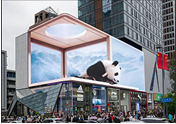
\includegraphics[width=0.9\linewidth, height=4cm]{resources/1p/1-1a.png}
    
    \centering\small(a)
    \label{fig:1-1a}
  \end{minipage}
  \hfill
  % 第二张子图
  \begin{minipage}{0.49\textwidth}
    \centering
    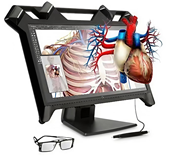
\includegraphics[width=0.9\linewidth, height=4cm]{resources/1p/1-1b.png}
    
    \centering\small(b)
    \label{fig:1-1b}
  \end{minipage}

  \vspace{0.5cm}

  % 第三张子图
  \begin{minipage}{0.49\textwidth}
    \centering
    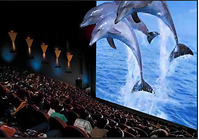
\includegraphics[width=0.9\linewidth, height=4cm]{resources/1p/1-1c.png}
    
    \centering\small(c) 
    \label{fig:1-1c}
  \end{minipage}
  \hfill
  % 第四张子图
  \begin{minipage}{0.49\textwidth}
    \centering
    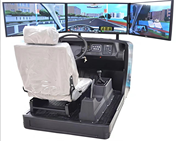
\includegraphics[width=0.9\linewidth, height=4cm]{resources/1p/1-1d.png}
    
    \centering\small(d) 
    \label{fig:1-1d}
  \end{minipage}

  \caption{三维显示技术的典型应用场景 (a)3D广告 (b)三维医疗 (c)3D电影 (d)三维模拟驾驶}
  \label{fig:1-1}
\end{figure}

  



当前，日常生活中主流的显示方式仍以二维平面显示为主导。这种显示模式无法为观察者提供有效的深度感知信息，仅能呈现三维场景的单一视角投影，导致深度维度信息的缺失，限制了人们对客观事物的全面认知。在工业造型设计、户外广告传媒、医学教育培训以及军事仿真作战等诸多应用领域，三维显示技术\cite{Hua2022}展现出广阔的发展前景。能体现出更真实\cite{李涵宇2025}的效果，作为下一代显示技术的核心演进方向，三维显示正在加速向生产生活各领域渗透\cite{Li2023}。

从工业制造到商业推广，如图所示该技术体现出显著的应用价值：在商业广告领域，如图~\ref{fig:1-1}(a)所示，三维显示技术重构了广告传播的呈现形式。相较于传统二维广告的平面化表达，三维广告能够精准还原产品的立体结构、细节纹理及空间形态，借助光影渲染增强视觉层次感\cite{Wang2021a}，既能够让受众直观感知产品核心优势，又能通过沉浸式视觉体验吸引注意力，有效提升广告传播效率，助力企业强化品牌认知，进一步推动产品转化率的提升，成为当下商业营销升级的重要突破口。在三维医疗领域，如图~\ref{fig:1-1}(b)所示，三维显示技术为医学诊疗与研究提供了有力支撑\cite{Chen2022}。该技术可将医学影像数据转化为逼真的三维立体模型，精准还原人体器官、组织的空间位置关系、形态结构及病变区域\cite{Zhang2020}，帮助医师更清晰地把握病灶特征，不仅大幅缩短术前规划时间、提升手术精准度，还能为医学教学、病例研讨提供直观的可视化载体，助力医学人才培养和诊疗技术的革新。在三维电影领域，如图~\ref{fig:1-1}(c)所示，三维显示技术推动了影视产业的业态升级\cite{Hu2022}。通过模拟人眼双目视觉原理\cite{Yang2021}，三维电影能够构建出立体逼真的影视场景，让观众突破屏幕局限，获得“身临其境”的观影体验，既丰富了影视内容的呈现形式，又增强了作品的视觉感染力，推动影视产业从二维向三维转型，带动了影视制作、放映等相关产业链的协同发展。在三维模拟驾驶领域，如图~\ref{fig:1-1}(d)所示，三维显示技术成为驾驶培训与研发的核心支撑\cite{Liu2022}。该技术可精准构建复杂的道路环境、交通场景及车辆运行状态，还原不同天气、路况下的驾驶场景\cite{Zhang2022a}，既能够为驾驶学习者提供安全、高效的模拟训练环境，降低实操培训风险和成本，又能为车辆研发、交通管控系统优化提供可视化模拟平台，助力提升驾驶安全水平和交通管理效能。

随着显示技术的进步，3D显示技术有了很大的进步，目前能够商用的显示技术主要分为需要佩戴外部设备的3D显示\cite{Sun2021}和不需要佩戴外部设备的裸眼3D显示技术，如图\ref{fig:1-2}所示：

\begin{figure}[htbp]
  \centering
  % 第一张子图（上方）
  \begin{minipage}{0.8\textwidth}  % 宽度保持和原格式一致，也可改为0.8\textwidth让图更宽
    \centering
    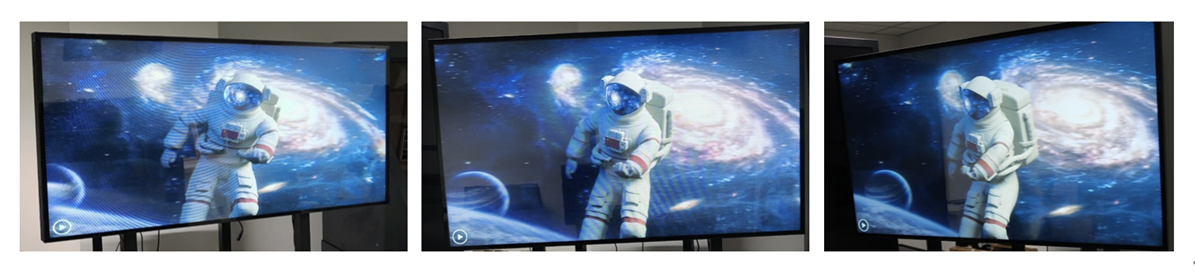
\includegraphics[width=0.9\linewidth, height=3cm]{resources/1p/1-2a.png}
    
    \centering\small(a)
    \label{fig:1-2a}
  \end{minipage}

  \vspace{0.5cm}  % 上下子图的间距，比原0.5cm稍大更美观，可按需调整

  % 第二张子图（下方）
  \begin{minipage}{0.8\textwidth}
    \centering
    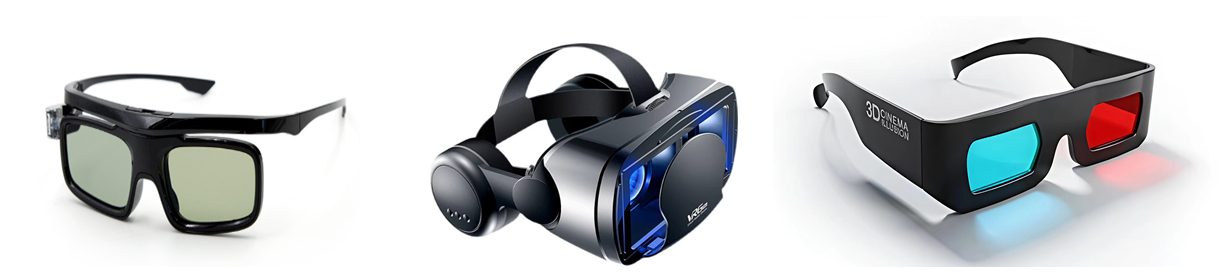
\includegraphics[width=0.9\linewidth, height=3cm]{resources/1p/1-2b.png}
    
    \centering\small(b)
    \label{fig:1-2b}
  \end{minipage}

  % 大图标题：仅保留两张子图的说明
  \caption{ (a)裸眼显示 (b)助眼显示}
  \label{fig:1-2}
\end{figure}

裸眼3D显示与传统需要佩戴专用辅助设备的三维显示方式存在显著区别，裸眼3D显示技术在不需要任何辅助设备的前提下，即可直接向观看者呈现立体视觉效果。相较于传统佩戴式三维显示，裸眼三维显示不仅彻底摆脱了辅助设备带来的佩戴束缚，避免了长时间佩戴设备产生的眩晕感、不适感，大幅提升了观看的便捷性和舒适度；还打破了佩戴设备对观看人数、观看场景的限制，无需观看者额外携带或佩戴相关器材，可支持多人同时观看，适配更多公共场景和私人场景，降低了三维显示技术的应用门槛，进一步拓宽了其应用范围，为三维显示技术的普及和多领域深度应用奠定了坚实基础。

在真实物理空间中，物体表面的明暗变化主要由入射光方向、强度以及材质反射特性共同决定。合理的光照与阴影分布不仅能够揭示物体的几何结构，还能够强化空间层次与体积感，使观察者在视觉上更容易感知深度关系与空间位置。

光线对人像立体感的塑造效果差异显著。在有合理光照的人像中，光线在面部形成自然的明暗过渡，突出额头、鼻梁、颧骨等高光区域，并在眼窝、鼻底、下颌下方形成柔和的过渡阴影，清晰还原了面部骨骼结构与肌肉起伏，使人像轮廓饱满、层次分明，呈现出强烈的立体感与真实的空间质感；而在无明显光照的对比图像中，面部明暗变化微弱，缺乏光影对比，整体显得扁平单调，难以体现出人脸应有的三维结构与体积感，如图 \ref {fig:1-3} 所示。

\begin{figure}[htbp]
  \centering
  % 第一张子图（左侧）
  \begin{minipage}{0.48\textwidth}  % 宽度减半，为左右排列留出空间
    \centering
    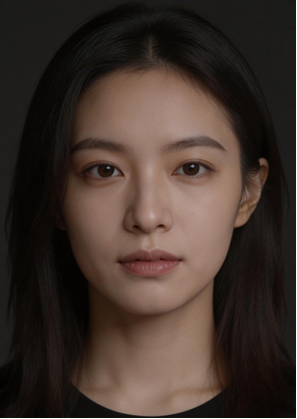
\includegraphics[width=0.9\linewidth, height=8cm]{resources/1p/1-3a.png}
    
    \centering\small(a) 
    \label{fig:1-2a}
  \end{minipage}
  \hfill  % 关键：添加水平间距，让两张图左右分开
  % 第二张子图（右侧）
  \begin{minipage}{0.48\textwidth}
    \centering
    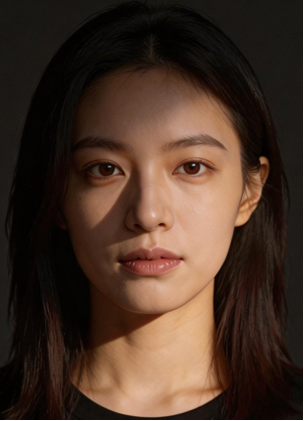
\includegraphics[width=0.9\linewidth, height=8cm]{resources/1p/1-3b.png}
    
    \centering\small(b) 
    \label{fig:1-2b}
  \end{minipage}

  % 大图标题：保持不变
  \caption{ (a)无光照的人像 (b)有光照的人像}
  \label{fig:1-3}
\end{figure}

由此可见，合适的光线与阴影分布是凸显人像立体感、还原真实空间形态的关键因素。这一规律同样适用于三维光场显示系统。与传统二维显示不同，三维光场显示通过重建多视角光线分布来还原真实场景中的光线传播状态，而光照信息正是其中决定真实感与沉浸感的核心要素之一。若光照方向错误或强度分布不合理，即使几何结构准确，也会导致画面失真、层次模糊，进而削弱立体感与空间可信度。

在静态三维光场人像显示中，光照的作用首先体现在对面部结构与细节纹理的塑造上。面部的高光区域、阴影过渡以及环境光的柔化效果能够清晰勾勒五官轮廓，突出鼻梁、颧骨与下颌线等关键结构，从而增强视觉立体度与真实度。适当的侧光或顶光可以有效提升人物的空间分离度，使主体从背景中自然凸显出来。同时，通过对光照颜色与强度的精确编辑，还能够传达情绪氛围与艺术风格，实现技术真实与视觉美感之间的平衡。因此，在静态光场人像重建与显示过程中，光照编辑不仅是一种后期增强手段，更是一种直接影响三维感知质量的基础环节。

而在动态三维光场人脸视频显示中，光照的重要性进一步放大。与静态场景相比，动态视频不仅包含空间维度变化，还叠加了时间维度上的连续运动信息。此时，光照的一致性、时序稳定性以及物理合理性将直接影响观看者的连续视觉体验。如果相邻帧之间光照分布突变或阴影跳变，将产生明显的闪烁与违和感，破坏沉浸效果，甚至引发视觉疲劳。因此，动态光照编辑需要在保证物理一致性的前提下，实现跨帧光照平滑过渡与多视角协同一致，以维持整体场景的真实连续性。

综上所述，无论是静态三维光场人像显示还是动态三维光场人像视频显示，光照始终是构建立体真实感与空间可信度的关键因素。光照编辑不仅影响单帧画面的明暗层次与几何表现，还决定了跨时间维度的视觉连贯性与沉浸体验质量。在三维光场显示研究与系统实现中，光照编辑是提升整体显示效果与用户感知质量的必要路径。

然而，现有三维光场人像光照编辑方法在实际应用中仍面临诸多挑战，比如采集设备繁琐，系统成本高昂，或者是编辑结果缺乏真实感，多视角一致性不足等问题。基于此，本课题聚焦三维光场显示中的人脸光照编辑，开展深入研究与创新，旨在为三维光场显示提供、高质量的内容支撑。


\section{研究现状}
\subsection{三维光场静态人像光照编辑的研究现状}
近年来，三维光场技术取得显著进步，三维光场显示可以提供理想的立体视觉体验，观者在其中观看三维场景就像它们存在于真实空间一样。它能够提升虚拟现实等领域的用户体验，对于数字媒体和人机交互的发展起到重要影响\cite{Bruno2010,Ho2020,Yang2013}。真实空间中，物体的明暗分布取决于光照，光照与阴影可以凸显画面的深度\cite{陈嘉琪2018,Todd2025}。而在三维光场显示中，光照同样是增加 3D 显示真实感和空间感的重要因素，通过编辑光照，可以大大提升立体显示效果。而合理准确的光照对于三维光场的显示效果起到非常关键的作用，光照编辑是三维光场中用于调整三维光场显示效果的常用方法。目前，对于三维光场人像光照编辑有两种方式。分别是多视图同时编辑方法和基于光照条件的密集视点采集方法\cite{Yang2023}。
多视图同时编辑方法，本质是对单张人像进行编辑，如图\ref{fig:single}所示,通过对多张视差图同时进行光照编辑的方法，从而达到对三维光场人像的编辑。

\begin{figure}[htbp]
  \centering
  %\vspace{1 cm} % 使用该指令调整上下间距
  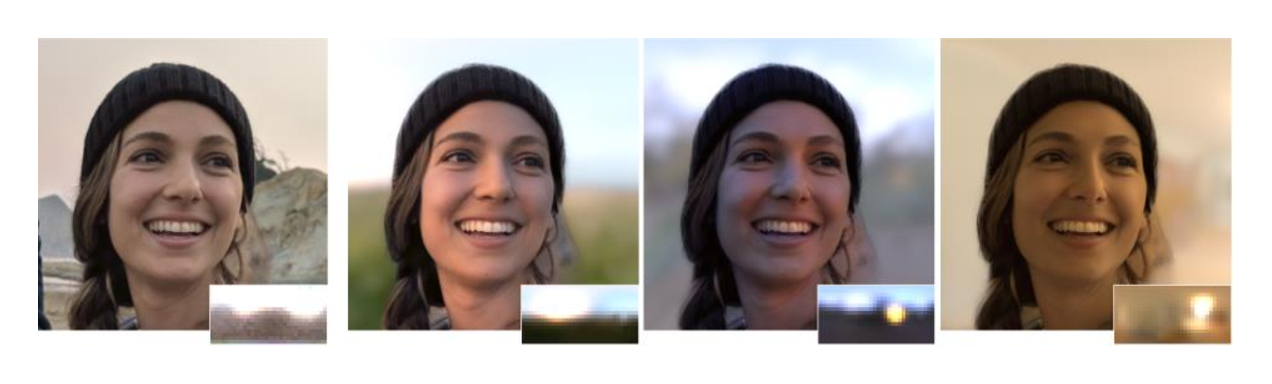
\includegraphics[width=0.7\textwidth,height=3cm]{resources/1p/1-single.pdf}
  % \bicaption{单张人像重光照}{English Caption} % 使用中英文标题
  \caption{单张人像重光照} % 只使用中文标题
  \label{fig:single}
  %\vspace{1 cm} % 使用该指令调整上下间距
\end{figure}

基于Chen提出的局部约束的全局优化实现光照编辑方法\cite{Chen2010}，是先构建局部光照约束，再通过全局优化算法调整整体光照效果，从而灵活改变人脸受光强度、方向等，实现自然的光照重新渲染。Liang提出的自适应编辑传播的人脸图像光照编辑\cite{梁凌宇2015}，通过融合参考人脸与目标背景、提取光照信息后，经自适应编辑传播生成光照模板并与目标人脸融合，实现光照编辑。Adobe Research 提出的SynthLight模型，将图像重光照建模转换成基于环境光照条件的像素重渲染问题，利用 Stable Diffusion\cite{Rombach2022}扩展的模型，并采用多任务训练策略和推理时的分类器自由引导机制，实现对 2D 人像的重光照\cite{Chaturvedi2025}。基于Xu等人提出了一种人像重光照系统，将标准手机相机拍摄的单张人像 RGB 图像作为输入，可生成在任意给定环境光照下的重光照图像，仅使用单个 RGB 肖像图和新的目标高动态范围照明环境作为输入就能实现更换背景重打光\cite{Sun2019}。基于商图像的多任务人脸光照编辑方法是通过预处理、商图像特征提取、特征扩散以及图像融合等步骤，在一个技术框架内同时实现人脸的光照迁移和重光照。IC-Light \cite{Zhang2025}方法基于光传输独立性原理，借助扩散模型\cite{Nichol2021,Rombach2022,Wang2024}和多层感知器，在训练中施加一致光传输约束，从而实现 2D 人像重光照。然而，三维光场内容由多视图构成，不同视图间的光照信息相互关联，当单独处理某一单张视图的光照时，会使多视图之间的光照一致性得不到保证,进而削弱三维光场的真实感与连贯性。

基于光照条件的密集视点采集方法如下，基于Paul 提出的light stage方法\cite{Debevec1999}，通过环形阵列光源依次点亮并同步拍摄，可采集人脸在不同光照条件下的高分辨率反射特性数据，可捕获数百乃至数千种不同光照方向、强度和颜色的面部反射数据，形成包含漫反射、镜面反射、次表面散射等多重物理特性的反射场\cite{Hanrahan1993}，结合 3D 几何模型实现后期任意角度的重光照渲染。上海科技大学 MARS 实验室提出的基于OLAT的采集方法，通过搭建由 114 个 LED 光源和一台 1000fps 的 4K 超高速摄像机组成的穹顶光场，在动态光照环境下可以达到更稳定人相重光照的视觉效果\cite{Zhang2021}。Shen提出的基于辐射场生成高质量光场人像的方法\cite{Shen2024}，能从任意视角和光照生成人像图像，通过分离场景几何和光照信息，生成高质量光场人像重光照结果，但是需要带偏振片的拍摄设备\cite{沈圣2025}。谷歌提出的人像照明技术，使用安装在球面内的 331 个 LED 灯进行拍摄，每次打开一个 LED 灯记录一个独立的光照结果，并利用 多个相机在不同的角度采集人物的多视图\cite{Goto2019}。Lu提出的通过环形或半球形部署的 48 台高性能相机形成密集视点采样网络\cite{Lu2014}，结合外围和顶部多组独立调控的 LED 光源构建自定义光照条件，同步采集不同光照下的密集视点人像数据，从而获取带光照的人像信息。上述光照条件的密集视点采集方法可以保证较好的多视图之间的光照一致性，但是需要搭建大规模数据采集设备。

 
\subsection{三维光场人脸视频动态光照编辑的研究现状}
在三维光场动态人像显示中，光照同样决定了场景的明暗关系与深度感，其分布的合理与否直接影响最终的视觉真实度，而人像视频的动态光照编辑是三维光场中用于调整三维光场人像视频显示效果的常用方法。目前，针对三维光场人像视频动态光照编辑的方法主要有如下三种，分别是基于静态三维光场人像光照编辑的直接动态扩展，基于三维重建的编辑方法和基于动态光照条件的密集视点视频采集方法。

\begin{figure}[htbp]
  \centering
  %\vspace{1 cm} % 使用该指令调整上下间距
  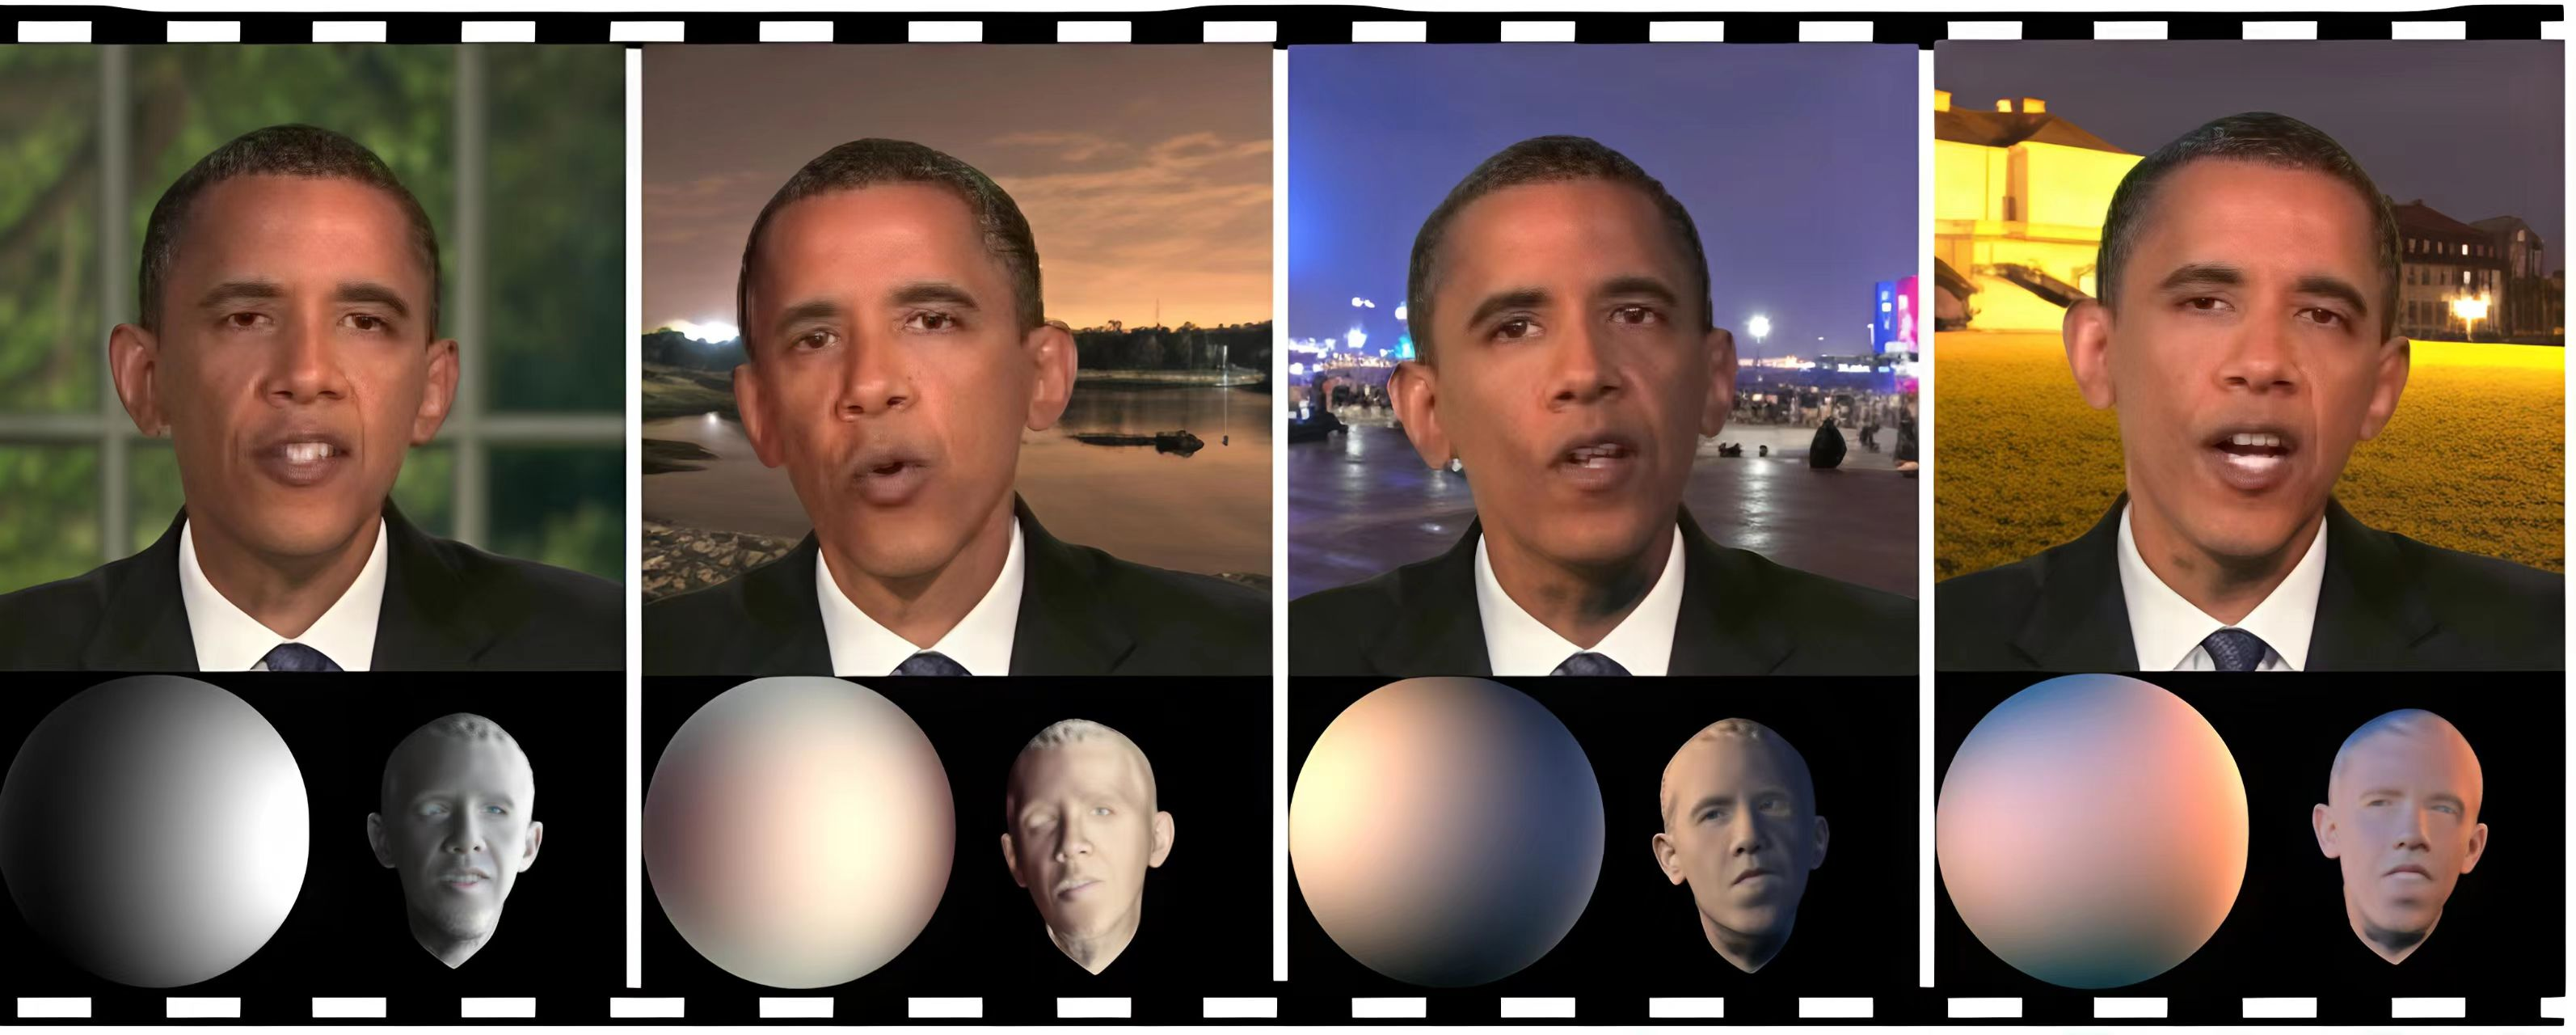
\includegraphics[width=0.7\textwidth,height=4cm]{resources/1p/1-5.jpg}
  % \bicaption{中文标题}{English Caption} % 使用中英文标题
  \caption{人脸视频重光照} % 只使用中文标题
  \label{fig:1-4}
  %\vspace{1 cm} % 使用该指令调整上下间距
\end{figure}
基于静态三维光场人像光照编辑的直接动态扩展，如图\ref{fig:1-4}所示，本质上是直接将单帧图像应用于视频序列，Chan\cite{Chan2022}通过估计人像的表面法线、反射特性与原始光照分布，再利用物理或学习模型在新的光照条件下重建图像，实现光源方向、强度或颜色的改变，从而生成具有目标光照效果的人像。Wang\cite{Ranjan2023}先由抠图模块从单张 RGB 图中提取前景；再经几何网、反照率网分别预测表面法向量与反照率，结合预过滤的漫反射和镜面光图构建像素对齐光照表示；最后由着色网合成含非朗伯效应的重光照结果，进行人像背景的重光照。Zhou\cite{Zhou2019}通过比率图像算法生成 DPR 数据集，用 3DDFA 估算法向量并经 ARAP 扭曲优化，结合 SfSNet 估计的球谐光照。再训练沙漏网络，以源图像和目标光照为输入，采用跳层训练策略，结合多损失函数正则化，最终生成 1024×1024 高分辨率重光照图像。Jiang提出的Nerflighting\cite{Jiang2023}框架，基于 EG3D 构建分离的几何外观潜空间与光照潜空间，通过光照映射网络将球谐系数转化为光照潜码，生成阴影三平面。结合正则化减少分解歧义、提升泛化性，经编码器投影真实人像至潜空间，实现动态光照编辑。Pan提出的ShadeGAN\cite{Pan2021}模型，模型显式解耦了反照率与3D形状。它利用表面法向结合输入的光照参数，通过朗伯着色模型计算像素颜色。仅改变输入的光照条件，即可实现静态人像重光照。然而，是上述方法为静态人像场景设计的，直接应用于视频时，会因为时序一致性差而产生帧间闪烁或和视频播放不自然的显示效果，难以满足三维光场视频显示中对平滑、逼真过渡的需求，并未对三维光场中特有的多视角一致性进行优化。

多视图人像视频同时编辑方法，其本质是对单目人像视频进行光照编辑，先获取到不同视角下的人像视频序列，然后依次使用相同的光照条件进行重光照，最后生成合成视频序列在三维光场上展示。基于Qiu\cite{Qiu2024}提出的提出 ReliTalk 框架，以单目视频为输入，借 FLAME 模型获初始面部几何与法向量，结合语音特征优化法向量图；动态估视频光照，分解反射率为法向量、反照率等；用身份一致性损失优化 3D 表示，最终实现单目人像视频重光照。Zhang提出的基于一致性建模的实时神经人像视频重光照\cite{Zhang2021b}以单目 RGB 视频为输入，构建含 60 余万帧的动态 OLAT 数据集，通过结构与光照解耦、时间建模及光照采样，联合保证语义等一致性，实现动态视频重光照。Wang提出Comprehensive Relighting\cite{Wang2025}框架，针对单目人体视频，依托预训练扩散模型构建粗到细框架，联合建模重光照与背景协调，引入无监督时序光照模型及时空特征融合、引导细化，实现多光照控制下连贯且泛化性强的人像视频重光照。Chandran提出首个端到端可微分的人像视频重光照\cite{Chandran2022}方法，针对单目人像视频逐帧重光照易产生闪烁的问题，联合优化目标光照与时间一致性。无需光照标注，利用现有人像视频训练，通过光照估计损失、时间损失和感知损失约束，结合面部对齐、重光照、合成与一致性网络，生成光照准确且时序连贯的人像视频重光照结果。上述方法是对视频人像进行光照编辑，可以保证较高的时序一致性，但是三维光场视频内容由多视图视频构成，不同视图间的光照信息相互关联，当单独对某一视角的视频序列进行光照编辑时，会使多视图之间的一致性得不到保证,进而削弱三维光场视频人像的真实感与连贯性。

密集视点人像视频现场采集方法如图\ref{fig:1-7}所示，是通过搭建自定义动态光照条件的密集视点采集设备，现场拍摄多视点的带动态光照的人像视频。ReN Human\cite{Xie2024}搭建约三十台同步相机与上百个可控光源组成的球形拍摄系统，通过逐光源点亮方式采集多视角、多光照条件下的人像视频。谷歌提出的The Relightables\cite{Guo2019}系统通过搭建一个包含 336 台高帧率相机与约 5000个可独立控制的 LED 光源的半球形穹顶拍摄装置，实现在多视角和多光照条件下的同步捕获。每一帧图像都对应一个精确记录的光照状态，所有视点同步记录，从而生成带有已知光照条件的多视角人像视频序列。Virtually Being\cite{Xu2025}使用约 75 台同步高分辨率相机 环绕搭建成多视角捕获阵列，并在外部配置 环形可编程 LED 光照系统。在采集过程中，系统通过时间复用光照控制依次激活不同方向与强度的光源，同时所有相机以毫秒级同步拍摄，从多个视角同时记录演员在不同光照条件下的反射与阴影变化。由此获得的包含光照变化信息的多视角视频序列。上述的密集视点人像视频现场采集方法可以得到更高时序一致性和多视角一致性的人像视频序列。但是需要搭建大规模采集设备和光源阵列，对于场地和时间的要求极高。

\begin{figure}[htbp]
  \centering
  % 第一张子图（左侧）
  \begin{minipage}{0.48\textwidth}  % 宽度减半，为左右排列留出空间
    \centering
    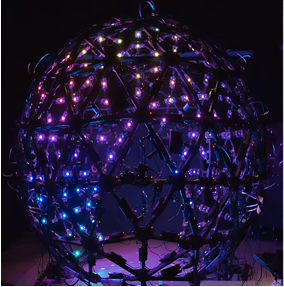
\includegraphics[width=0.9\linewidth, height=7cm]{resources/1p/1-7a.png}
    
    \centering\small(a) 
    \label{fig:1-2a}
  \end{minipage}
  \hfill  % 关键：添加水平间距，让两张图左右分开
  % 第二张子图（右侧）
  \begin{minipage}{0.48\textwidth}
    \centering
    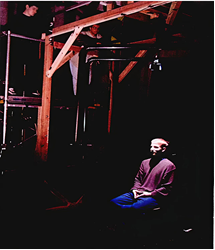
\includegraphics[width=0.9\linewidth, height=7cm]{resources/1p/1-7b.png}
    
    \centering\small(b) 
    \label{fig:1-7b}
  \end{minipage}

  % 大图标题：保持不变
  \caption{ (a) Relightables (b) lightstage}
  \label{fig:1-7}
\end{figure}
\section{论文的组织结构}
本文围绕面向三维光场人像光照编辑这一核心研究课题，立足三维光场显示的工程需求与技术痛点，遵循 “理论奠基 — 静态方法构建 — 动态优化升级 — 实验验证” 的学术逻辑，构建了层次清晰、逻辑闭环的研究框架。全文共分为六章，从基础理论、核心方法到实验验证逐步推进，形成完整的技术体系与学术论证链条，具体组织结构安排如下：

第一章题目是绪论。作为整篇论文的开篇，本章旨在明确研究背景、意义与核心目标，为后续研究奠定整体框架。首先，从三维显示技术的发展趋势切入，阐述裸眼 3D 光场显示的应用价值与市场需求，点明光照编辑在三维光场人像显示中的核心地位 —— 无论是静态场景下的立体结构塑造，还是动态场景下的沉浸感维持，光照均是决定真实感的关键因素。随后，系统梳理国内外研究现状，分别针对三维光场静态人像光照编辑与动态人像视频光照编辑两大方向，分析现有方法的优势与不足，针对当前研究中存在的 “采集设备复杂昂贵”“多视角光照一致性不足”“动态场景时序闪烁” 等核心问题，确立本文的研究切入点。在此基础上，界定研究范围与核心目标，提出具体研究内容：静态三维光场人像光照编辑基础方法、动态场景下时间和空间双维一致性优化策略。最后，给出全文章节组织结构，清晰呈现各部分的逻辑关联。

第二章题目是三维光场人脸光照编辑技术基础。本章是全文的理论基础，为后续方法设计提供科学依据与技术支撑。首先，从人类立体视觉的生理与认知机制出发，解析纹理梯度、透视关系、双目视差等核心深度线索，阐明三维光场显示的生物学原理；随后，详细讲解光场的数学定义与工程化模型，重点分析七维全光函数到四维双平面光场模型的降维逻辑，以及基于光栅的光场显示系统的结构、工作机制与关键参数计算方法。其次，深入阐述三维人像渲染的三大核心物理模型：相机投影模型、球谐函数光照模型（数学推导、展开方式及物理意义）、渲染模型（传统 PBR 渲染与 NeRF 体渲染的原理、优势与局限性）。最后，构建多维度客观评价指标体系，涵盖感知质量（FID、PSNR、SSIM、LPIPS）、WE、LE、LI等大类指标，明确各指标的计算方式与评价标准，为实验验证提供统一的量化依据。

第三章题目是三维光场人像静态光照编辑基础方法。本章作为核心方法的第一阶段，聚焦静态三维光场人像的光照编辑问题。首先，分析静态光场人像光照编辑的痛点：多视图独立编辑导致光照一致性差，密集采集设备成本高昂，因此提出 “关键信息驱动” 的核心思路 —— 通过提取光照关键信息（球面调和系数），在统一框架下实现多视角光照协同编辑。其次，设计完整的静态光照编辑框架，包含三大核心模块：高光去除模块、光照编辑模块、密集视点生成模块。最后，通过系统实验验证方法有效性：客观实验与 NVPR、LRPI 等主流方法对比，在 FID、PSNR 等指标上取得更优结果；主观实验基于三维光场显示器，通过 20 名参与者对 24 组场景的评估，证明方法在立体感（得票率 89.19\%）与光照一致性（得票率 92.29\%）上显著优于单视图依次编辑方法。本章为后续动态场景优化奠定了技术基础。

第四章题目是第四章 三维光场人脸视频动态光照编辑。本章作为核心方法的升级阶段，针对静态方法扩展至视频序列时出现的 “时序闪烁” 与 “多视角光照失配” 等问题，提出时间 - 空间双维联合优化框架。首先，时间维度上，逐帧编辑导致光照跳变；空间维度上，多视角独立优化破坏光照物理一致性。因此，构建两大核心优化模块：时序一致性优化模块（基于特征分离策略，通过共享编码器提取稳定语义特征，光流估计网络实现跨帧空间对齐，光照特征提取网络解耦几何与光照，双重损失函数约束光照时序连续）、多视角一致性优化模块（基于三维几何对齐，通过三维模型表面采样将多视角光照约束转化为三维点光照观测问题，多因子加权聚合获得统一光照值，一致性回投影优化还原至二维视角并保留细节）。最后，通过全面实验验证框架有效性：定量实验与 PTI、SMFR 等方法对比，在时序一致性与多视角一致性指标上的对比，以及时序一致性的消融实验验证模块的必要性，完整模型在所有指标上表现最佳；视觉效果展示证明方法在保留表情动态与细节纹理的同时，有效抑制了光照闪烁与视角偏移。

第五章题目是总结与展望。本章对全文研究工作进行系统性梳理与升华。首先，总结核心研究成果：提出了关键信息驱动的静态三维光场人像光照编辑方法，解决了设备复杂与光照不一致的问题；构建了时间 - 空间双维联合优化框架，突破了动态视频光照编辑的时序与多视角一致性瓶颈。客观分析研究局限性：目前仅适用于人像场景，对复杂非人像场景的适应性不足，实时性有待提升，难以满足高速动态视频的编辑需求。最后，展望未来研究方向：拓展多场景通用性，研究非人像场景的几何与光照解耦方法；优化实时推理性能，通过模型轻量化、硬件加速等方式提升处理速度；融合生成式 AI 技术，实现更精细的光照细节编辑与场景交互；探索多模态输入（文本、语音、草图）的光照编辑方式，进一步降低用户操作门槛。






%第一章
\chapter{三维光场人脸光照编辑技术基础}
光场技术能够同时记录光线“从哪里来、朝哪里去”，因此相比传统二维图像更适合表达真实三维场景。围绕这一能力，三维光场人脸光照编辑的目标可概括为：在跨视角一致与时间连续的前提下，重建并重塑人脸在复杂照明下的外观变化。本章从基础理论出发，对后续方法所需的关键知识进行重组，包括立体视觉感知机制、光场显示实现路径、光照与渲染物理模型以及定量评价体系。具体而言，先讨论人眼如何利用深度线索形成空间知觉，再介绍基于光栅的裸眼 3D 光场显示流程；随后梳理相机成像、球谐光照、传统渲染与 NeRF 体渲染等核心建模方法；最后给出 PSNR、SSIM、FID、LPIPS 等客观指标及其使用场景。与常规图像编辑任务不同，光场人脸光照编辑不仅要求单帧“看起来像”，还要求在视点切换时保持身份、几何和阴影逻辑不跳变，因此本章在组织上强调“感知机制—显示实现—物理建模—评价闭环”的递进关系。通过这种编排方式，后续章节可直接复用本章术语体系与评价口径，减少方法描述中的重复定义。同时，这种先理论后实现、先模型后评价的组织方式也便于读者在阅读实验章节时快速回溯到对应基础。上述内容共同构成本文第二章的理论底座。
\section{三维光场显示原理}
现有消费级显示设备大多仍停留在二维成像层面，空间深度需要依赖额外编码才能被观察者正确感知。人眼之所以能够“看出前后层次”，本质上是多种线索共同作用的结果。为便于分析，本文将其归纳为两组：一类是经验驱动的心理线索，另一类是由眼球结构与神经处理直接产生的生理线索。二者并非互斥关系，而是在观看过程中持续融合：当前景和背景纹理给出粗粒度深度判断时，双目系统会进一步给出更精细的距离修正；当显示系统参数不匹配时，心理线索与生理线索甚至可能出现冲突，从而引发观看疲劳。
\subsection{立体视觉原理}
(1)心理反应因素

在真实观看环境中，心理线索往往先于生理线索起作用：观察者会先根据画面构图和经验判断大致空间布局，再通过眼动与双目机制完成细节确认。因此，面向光场内容生产时，除了保证几何正确，还需要关注构图连贯、主体突出和阴影一致等“可读性”因素。

纹理梯度：如图\ref{fig:2-1}(a)所示，纹理单元沿深度方向的疏密变化会被视觉系统解释为距离变化，从而帮助观察者快速建立前后层级\cite{Gibson1950}。

透视关系：图\ref{fig:2-1}(b)对应经典透视规律。随着距离增加，目标在成像平面上的投影会按比例缩小，这一几何关系是二维画面传递纵深感的核心线索\cite{Kaufman2000}。

阴影分布：图\ref{fig:2-1}(c)显示，阴影轮廓和亮度过渡同时反映了光照方向与几何起伏。借助这些线索，观察者可以在单幅图像中推断局部凹凸关系\cite{Shafer1985}。
\begin{figure}[H]
  \centering
  % 第一张子图（左侧）
  \begin{minipage}{0.32\textwidth}  % 3张子图均分宽度，0.32*3≈0.96，留少量间距
    \centering
    
\includegraphics[width=0.9\linewidth, height=3.5cm]{resources/2p/2-1a.pdf}
    \centering\small(a)
    \label{fig:2-1a}
  \end{minipage}
  \hfill  % 子图间水平间距，自动均分空白
  % 第二张子图（中间）
  \begin{minipage}{0.32\textwidth}
    \centering
    
\includegraphics[width=0.9\linewidth, height=3.5cm]{resources/2p/2-1b.pdf}
    \centering\small(b)
    \label{fig:2-1b}
  \end{minipage}
  \hfill
  % 第三张子图（右侧）
  \begin{minipage}{0.32\textwidth}
    \centering
    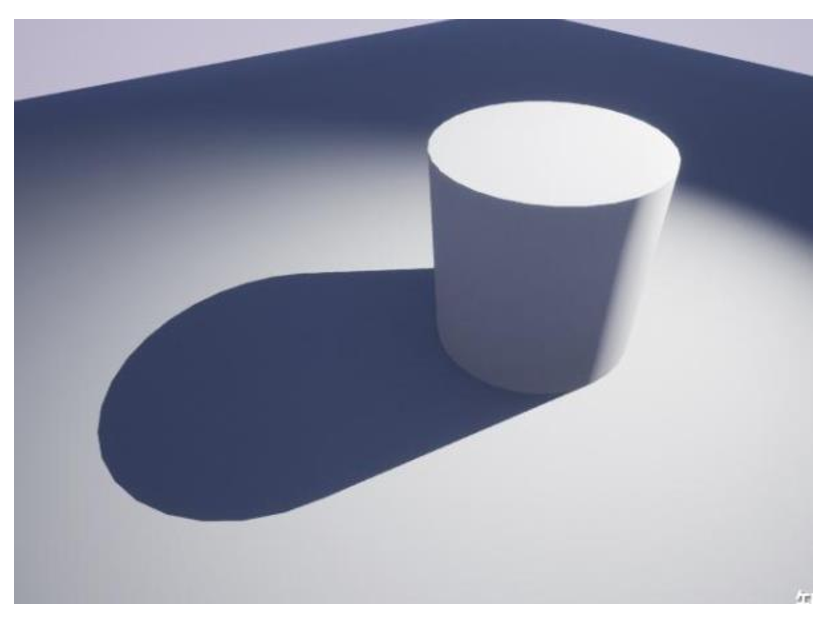
\includegraphics[width=0.9\linewidth, height=3.5cm]{resources/2p/2-1c.pdf}  % 替换为你的第三张图路径
    \centering\small(c)
    \label{fig:2-1c}
  \end{minipage}
  % 大图标题：补充第三张子图说明
  \caption{ (a)纹理示意图 (b)透视关系示意图 (c)阴影示意图}  % 替换XXX为你的第三张图说明
  \label{fig:2-1}
\end{figure}
(2)生理反应因素

与上述心理线索不同，生理线索由眼球成像与眼动控制直接产生，其中最关键的是双目视差\cite{Howard2002}。这也是三维显示系统设置视差与观看区参数时必须遵循的生物学基础\cite{Atchison2005}，如图\ref{fig:2-2}所示。

\begin{figure}[htbp]
  \centering
  % 第一张子图
  \begin{minipage}{0.49\textwidth}
    \centering
    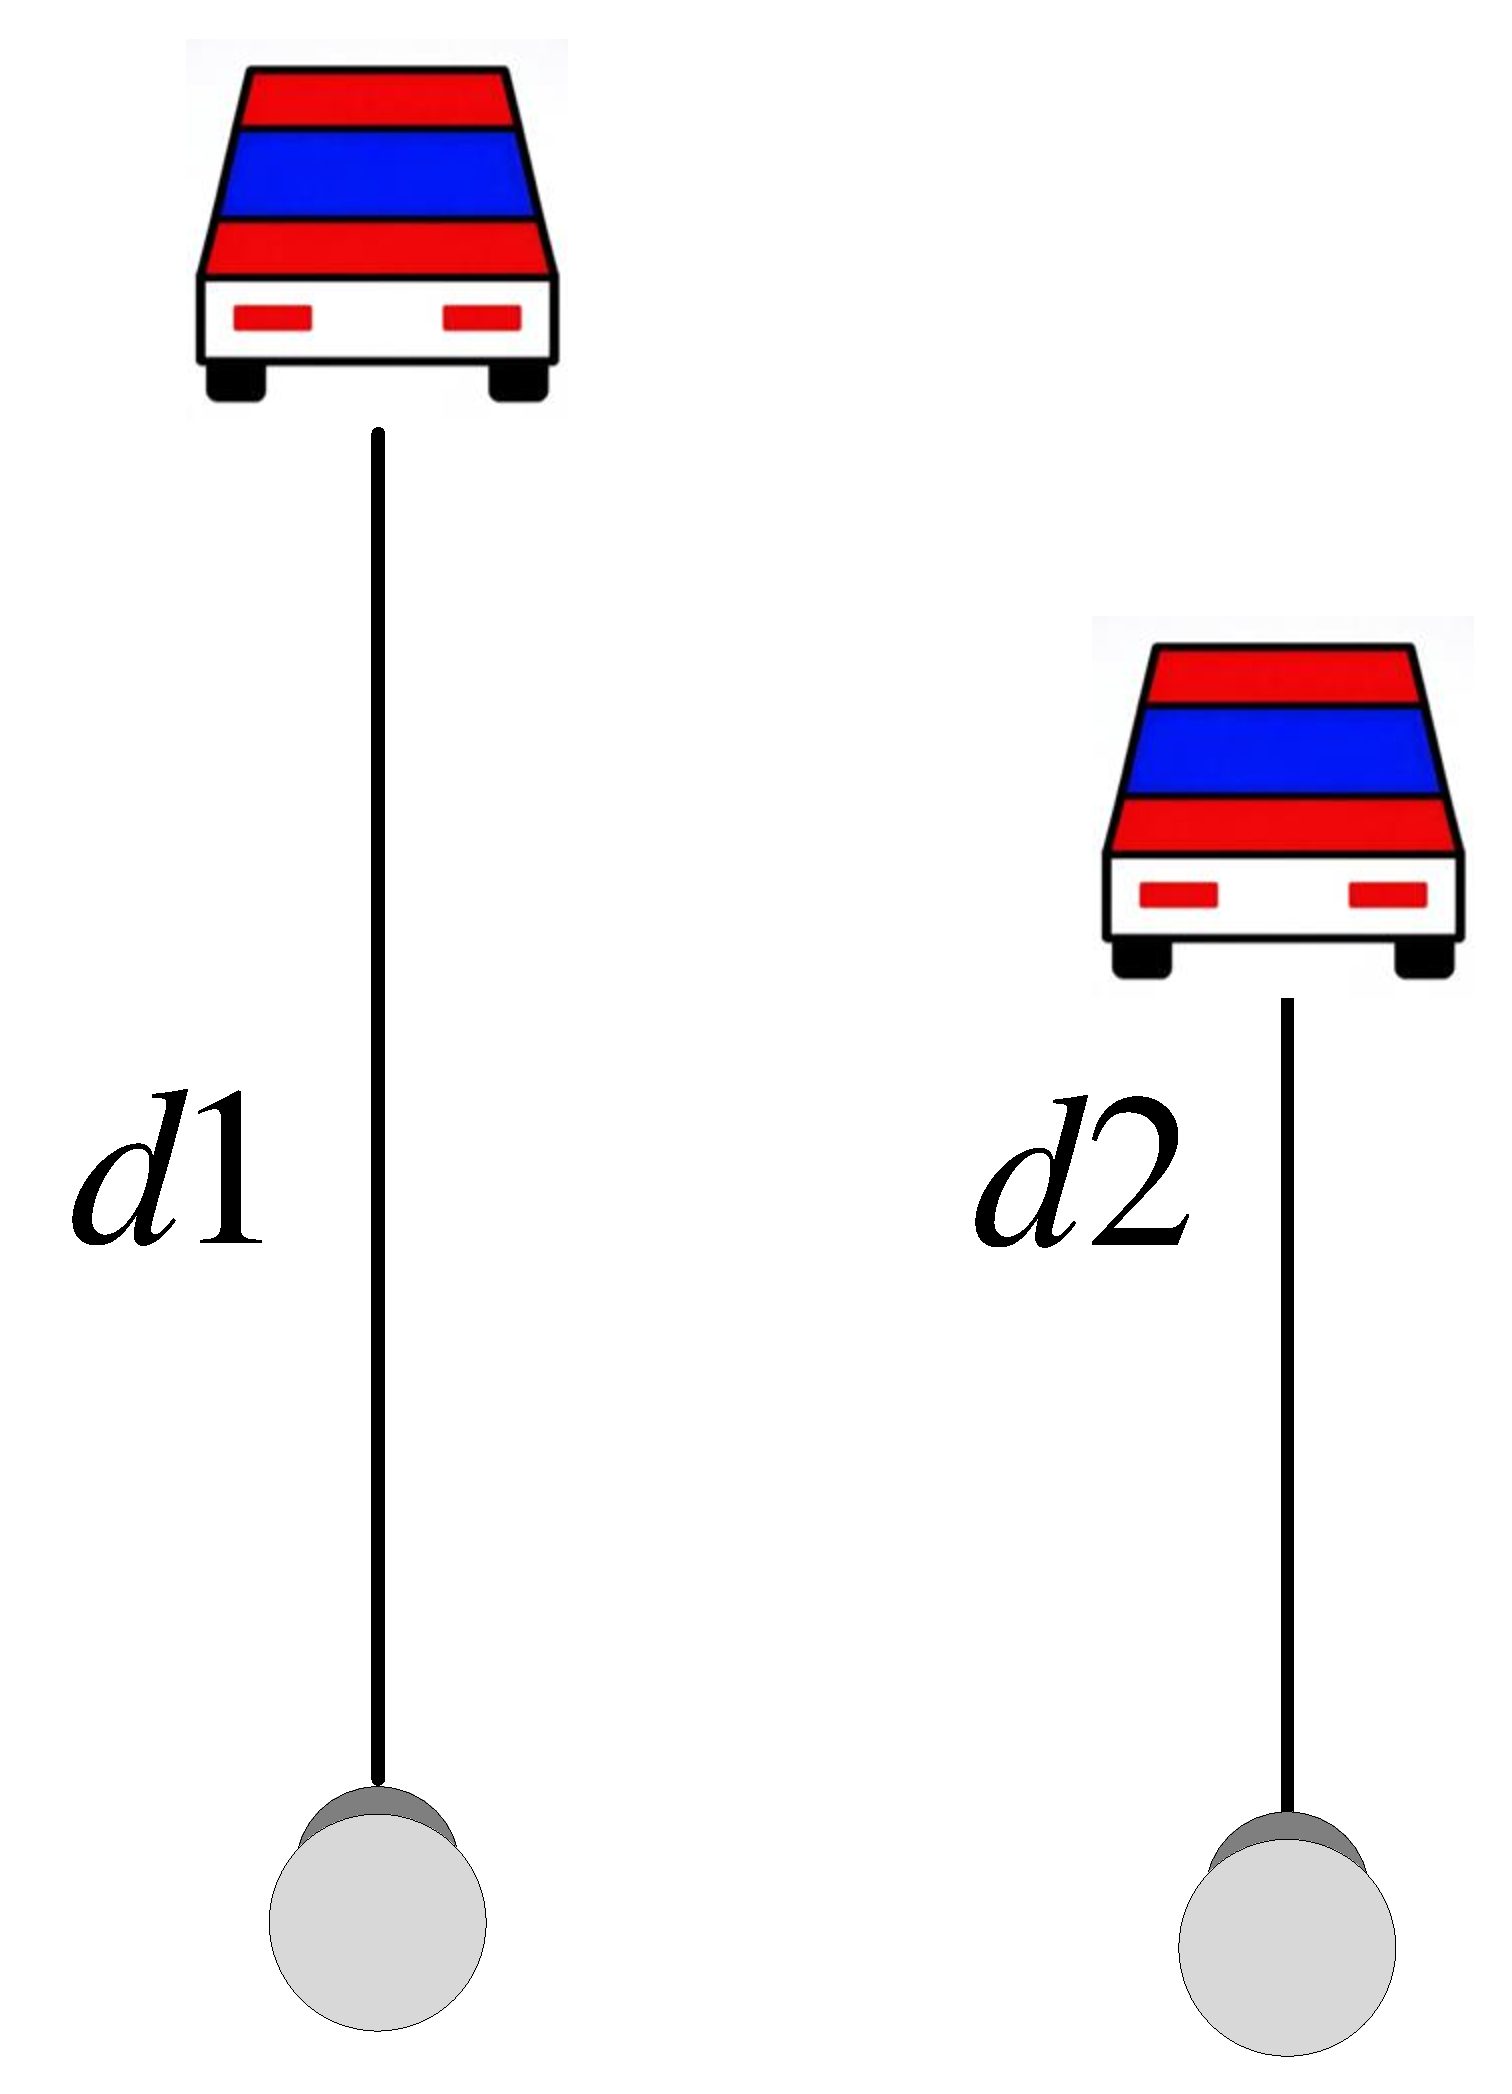
\includegraphics[width=0.8\linewidth, height=4cm]{resources/2p/2-2a.pdf}
    
    \centering\small(a)
    \label{fig:1-1a}
  \end{minipage}
  \hfill
  % 第二张子图
  \begin{minipage}{0.49\textwidth}
    \centering
    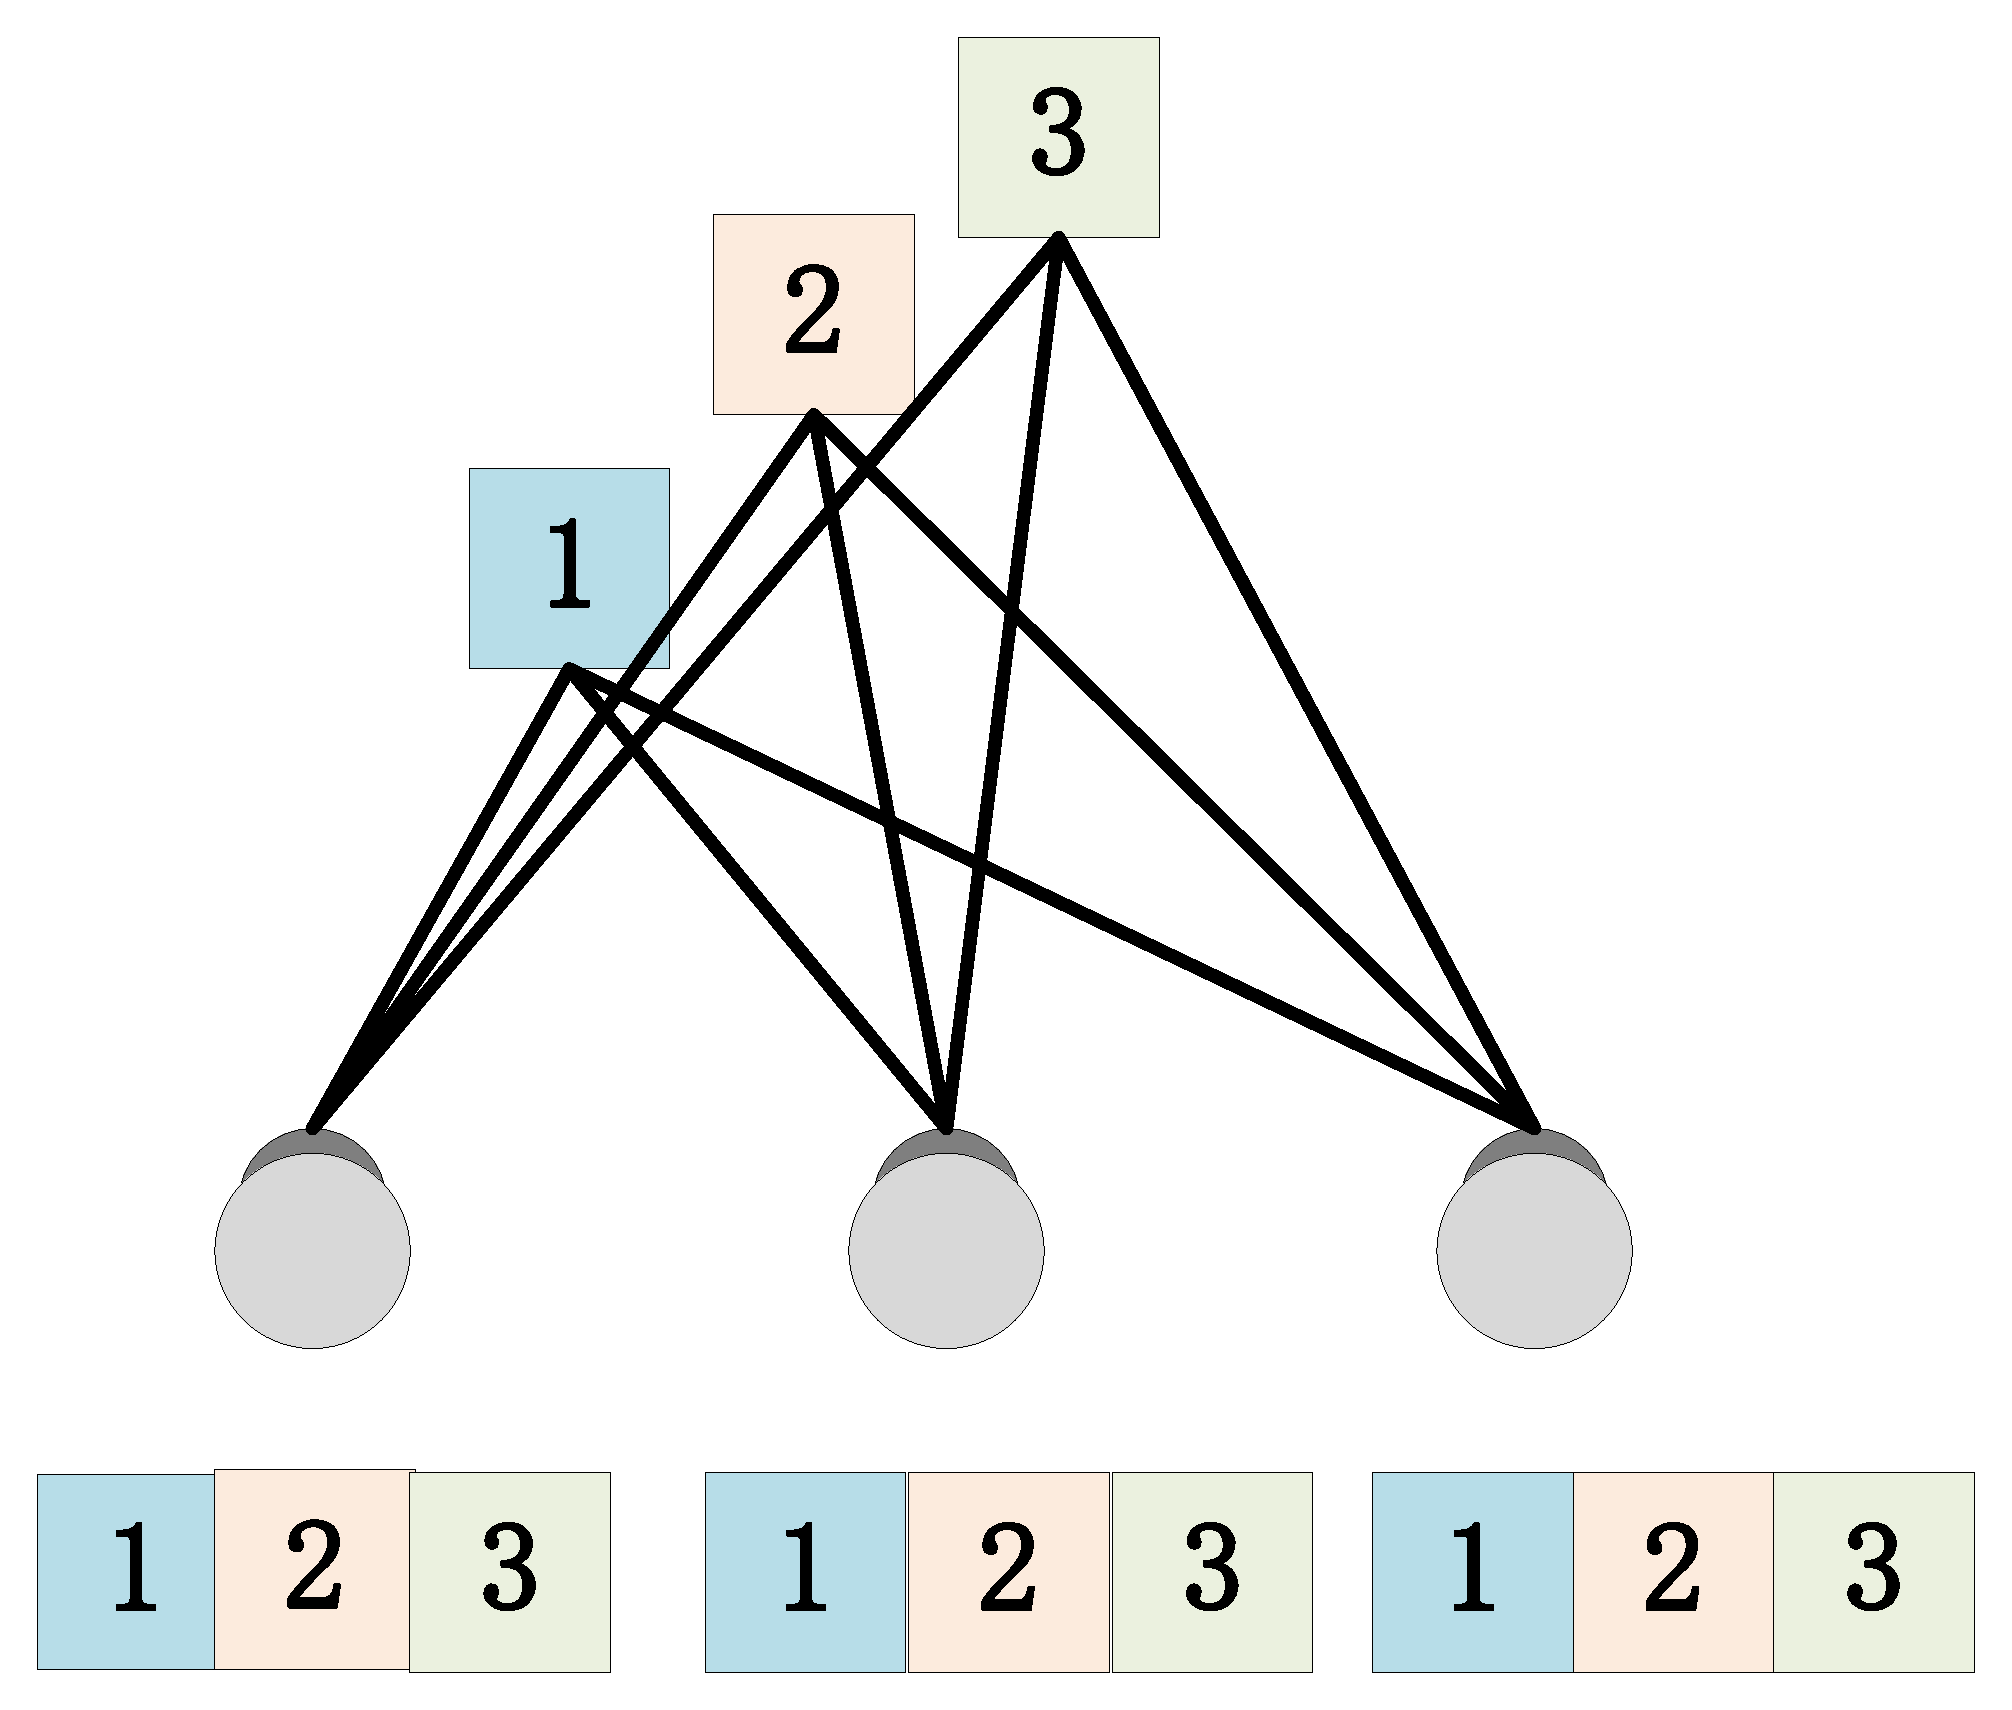
\includegraphics[width=0.9\linewidth, height=4cm]{resources/2p/2-2b.pdf}
    
    \centering\small(b)
    \label{fig:1-1b}
  \end{minipage}

  \vspace{0.5cm}

  % 第三张子图
  \begin{minipage}{0.49\textwidth}
    \centering
    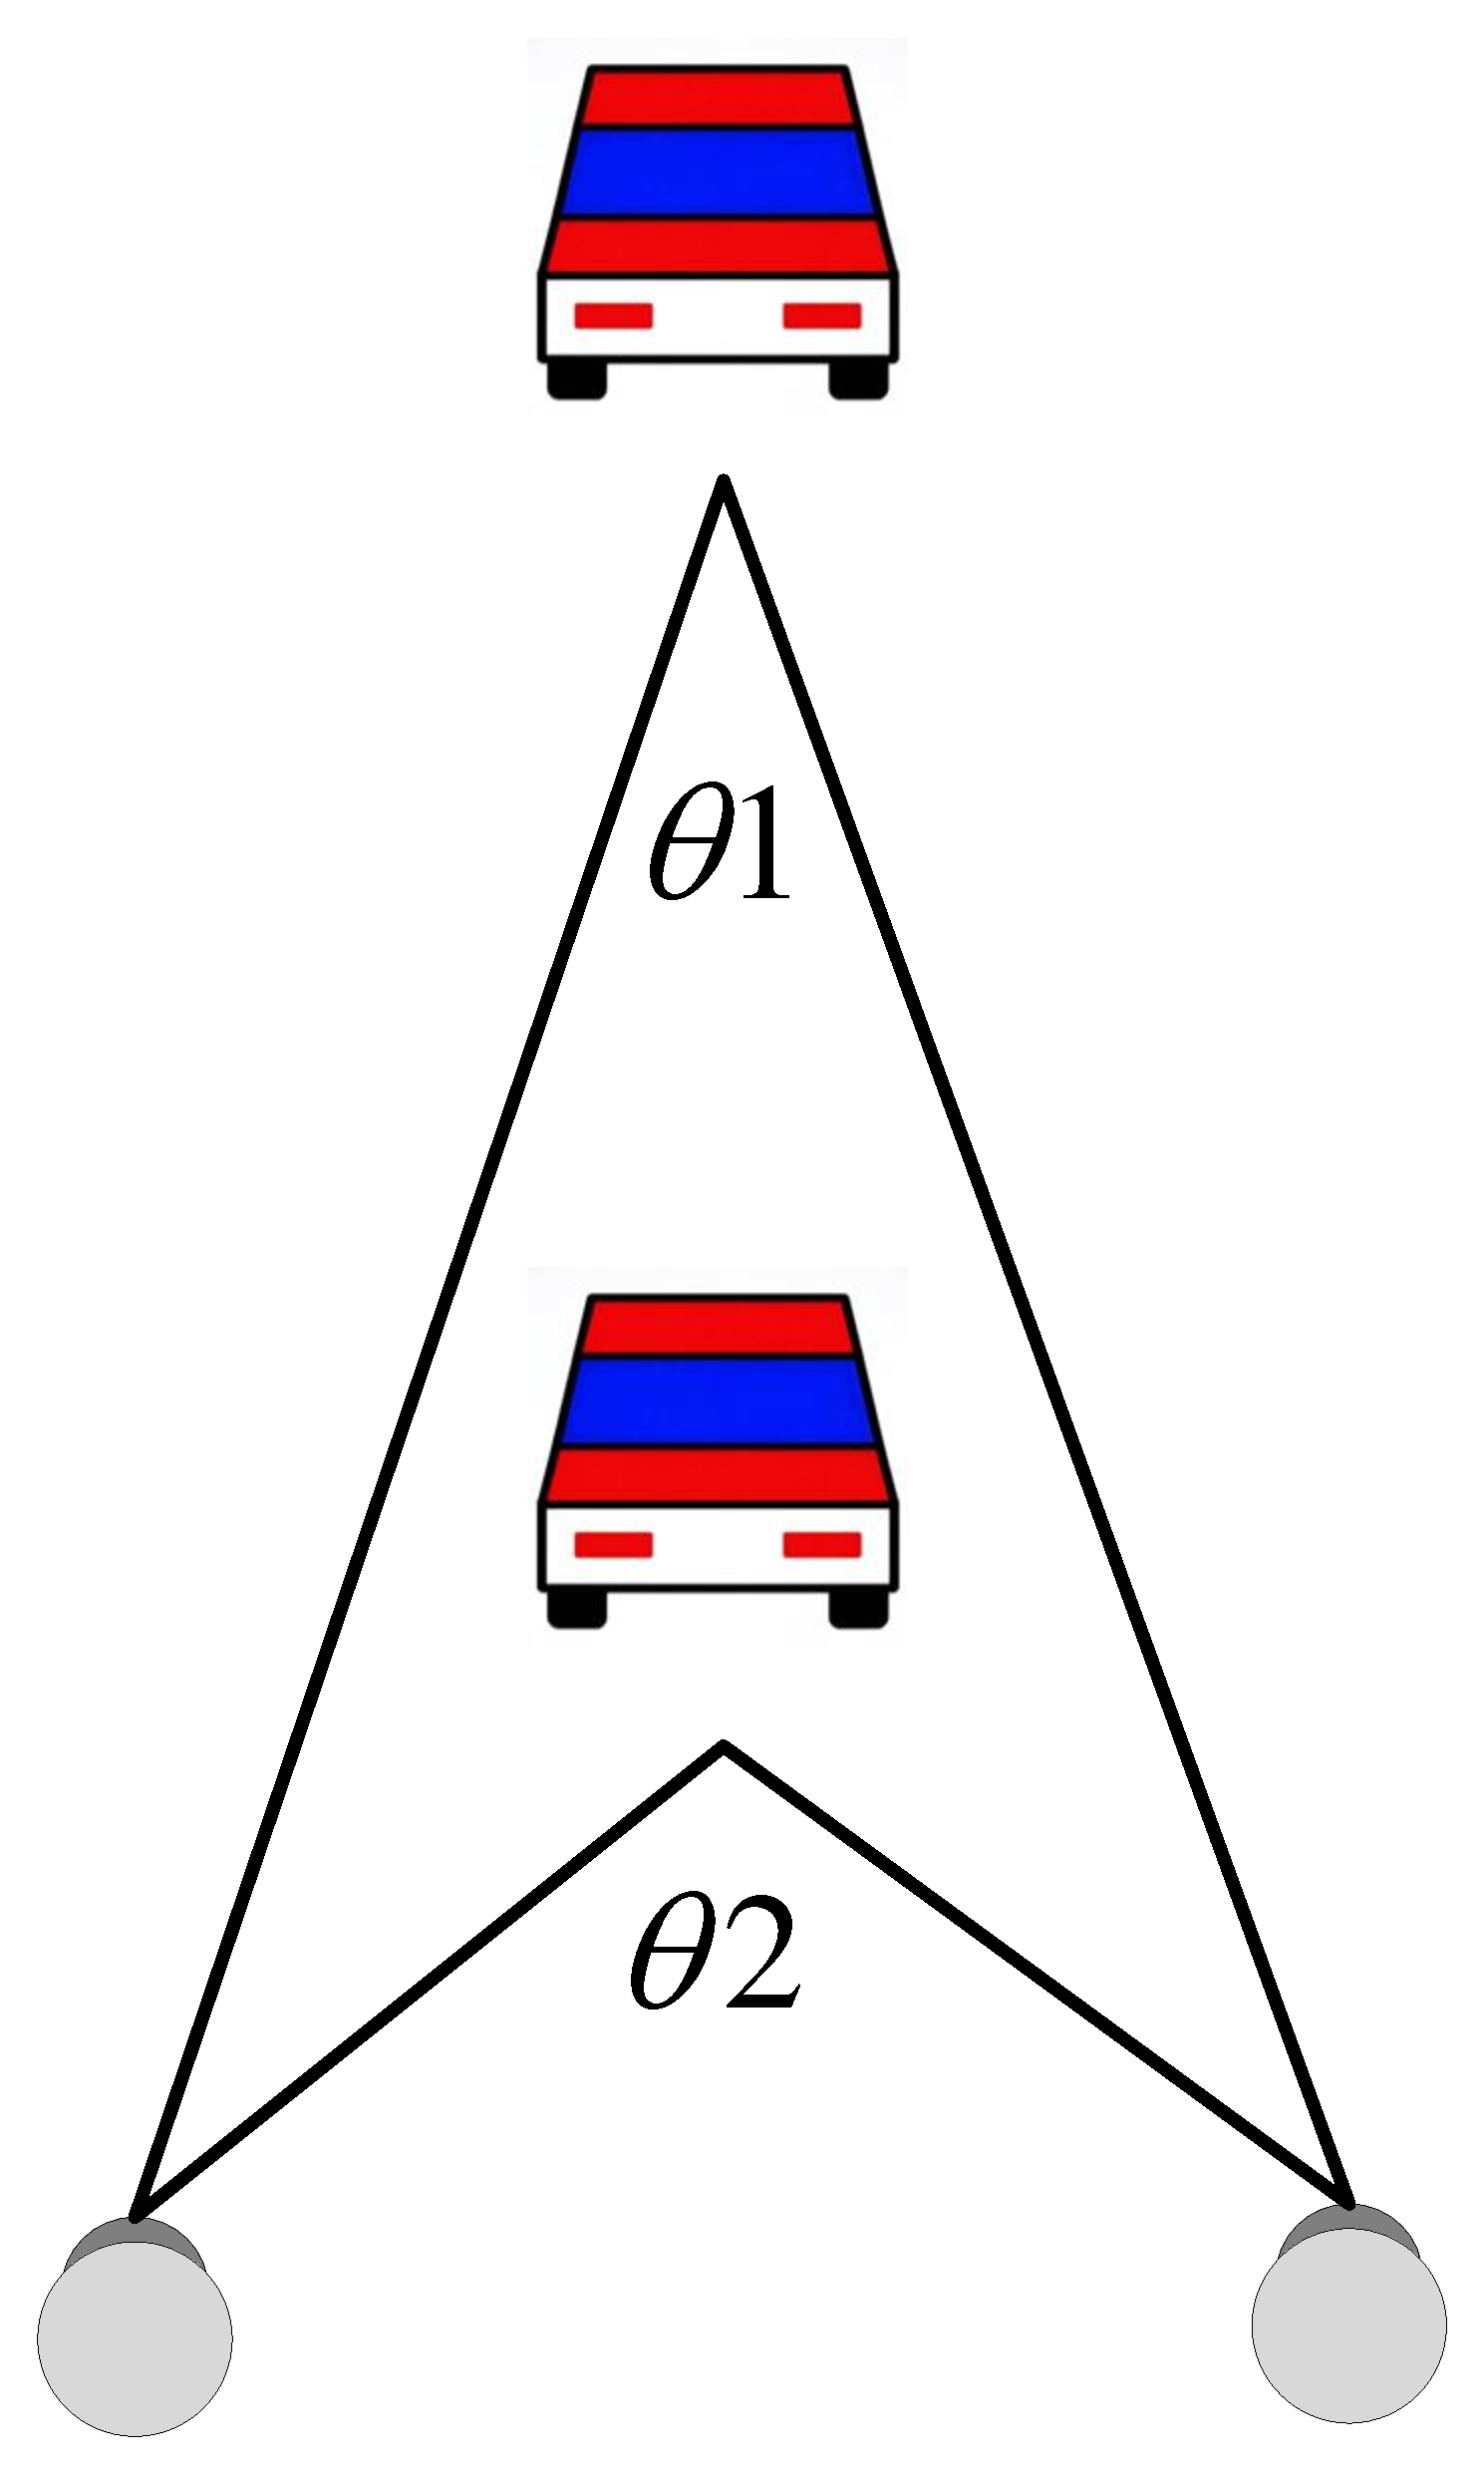
\includegraphics[width=0.8\linewidth, height=4cm]{resources/2p/2-2c.pdf}
    
    \centering\small(c) 
    \label{fig:1-1c}
  \end{minipage}
  \hfill
  % 第四张子图
  \begin{minipage}{0.49\textwidth}
    \centering
    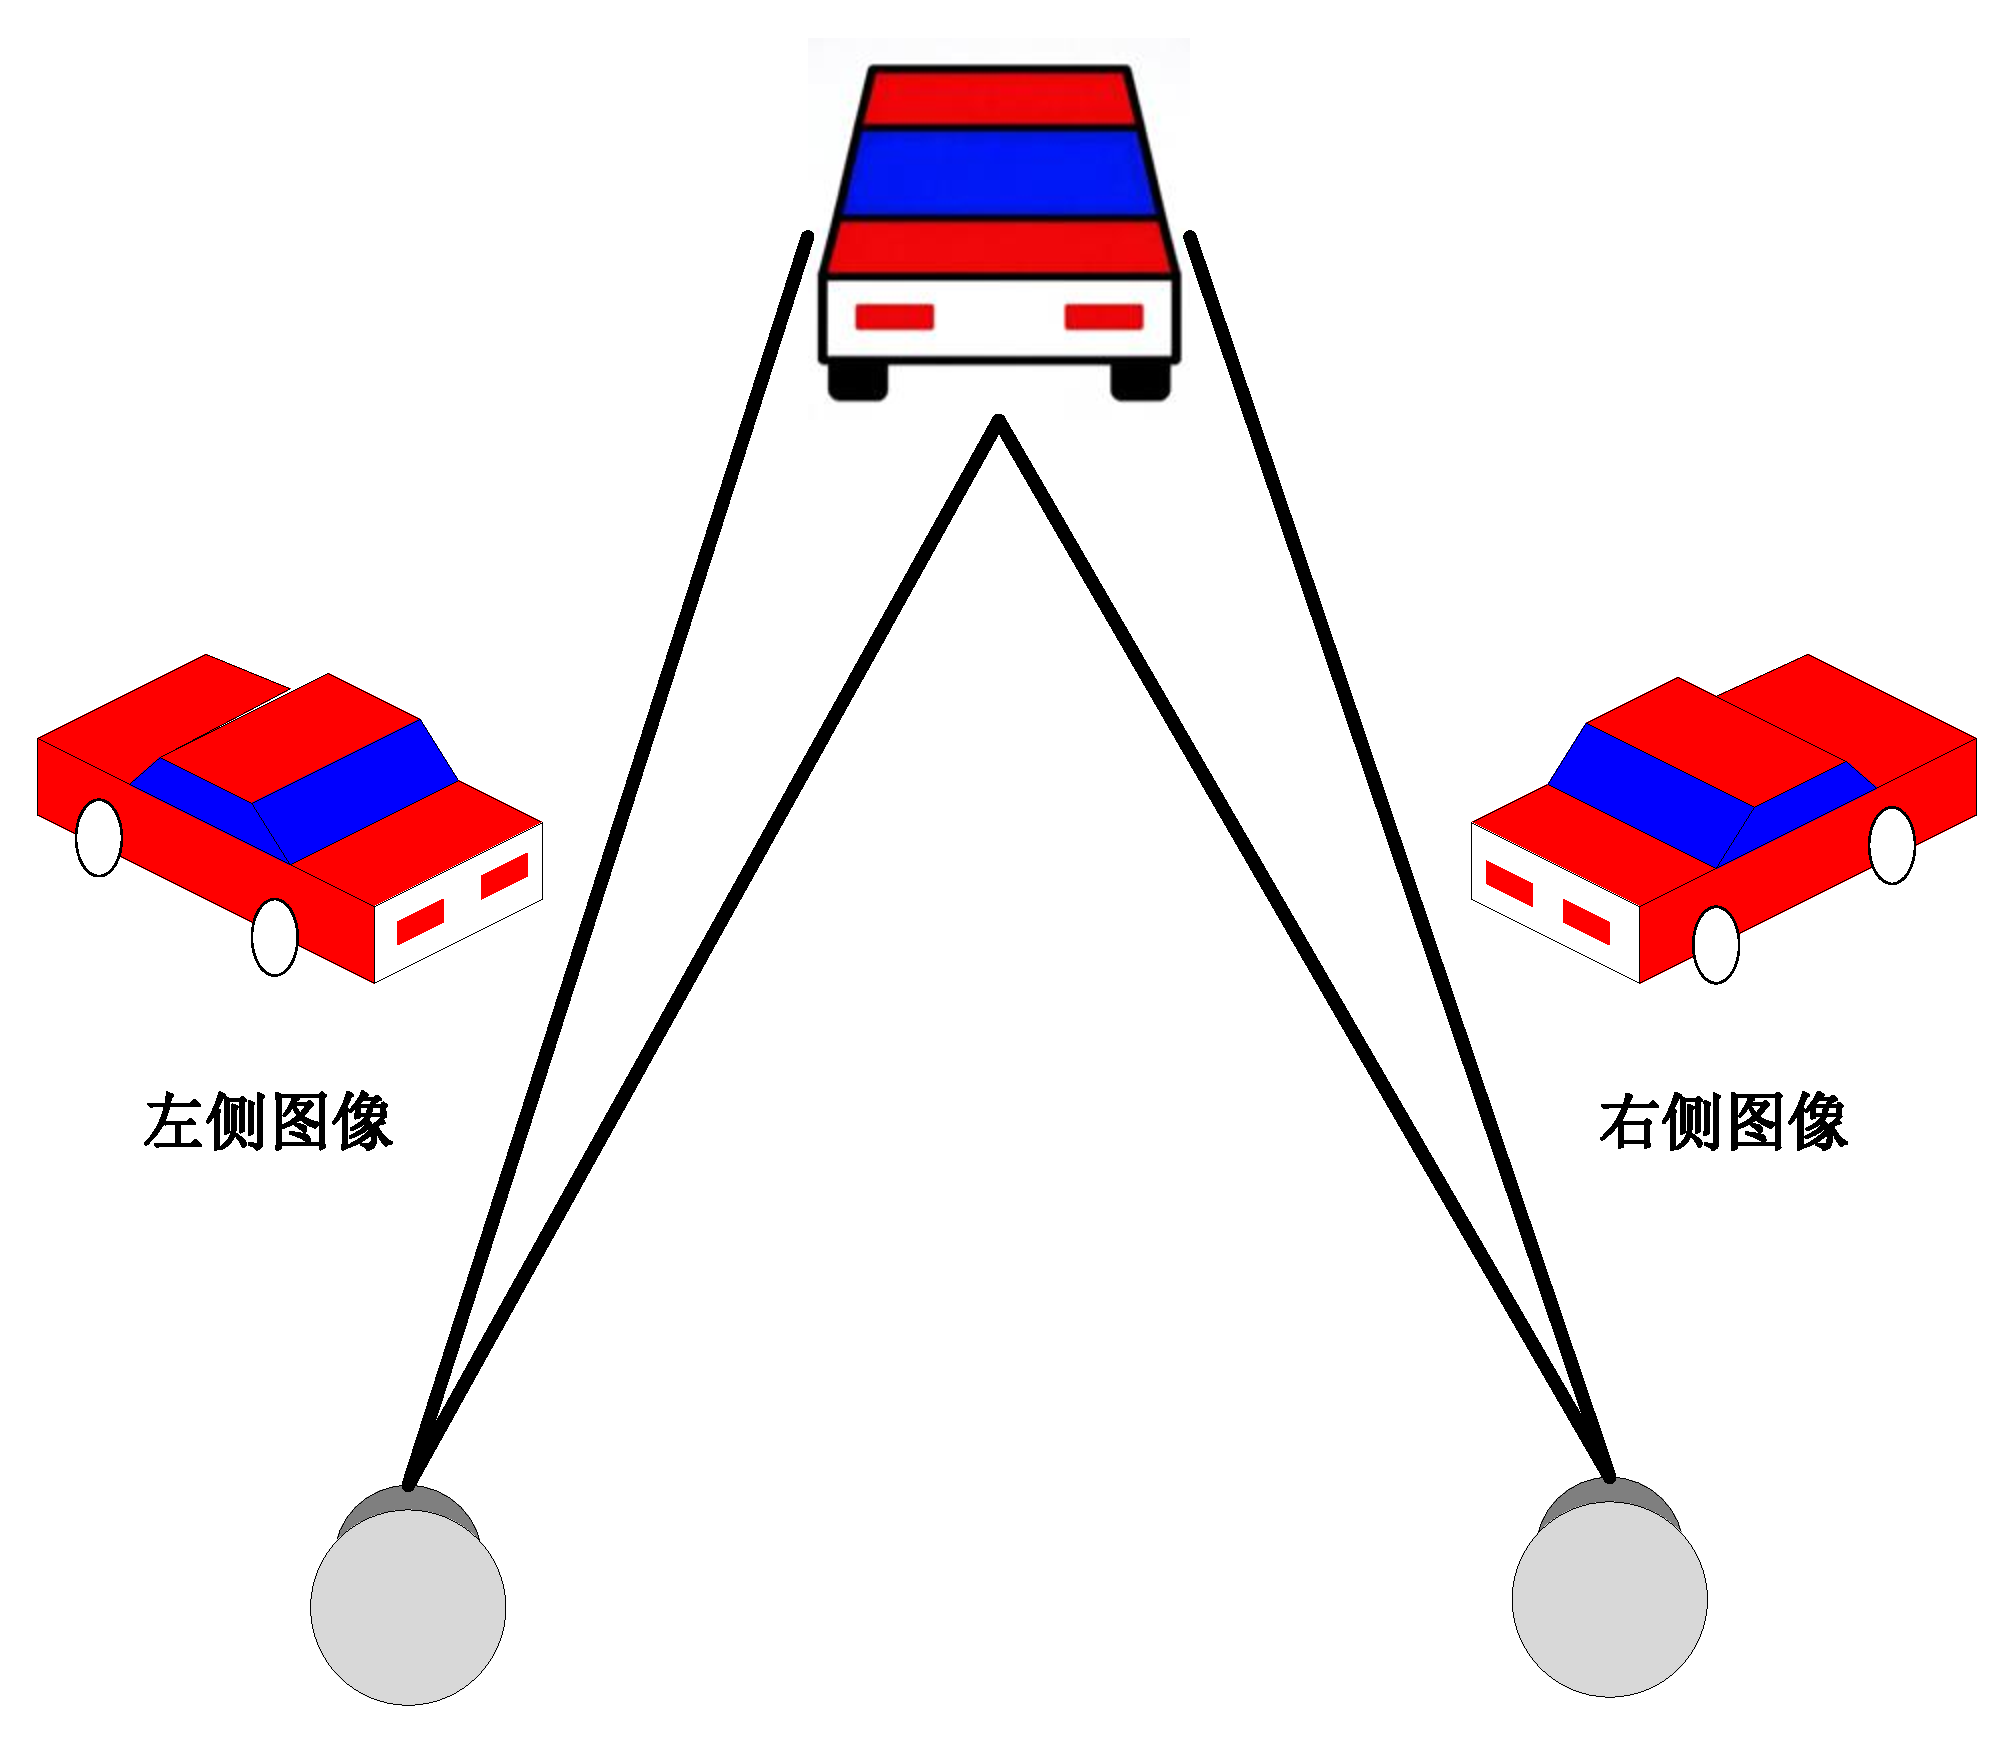
\includegraphics[width=0.9\linewidth, height=4cm]{resources/2p/2-2d.pdf}
    
    \centering\small(d) 
    \label{fig:1-1d}
  \end{minipage}

  \caption{ (a)调节机制示意图 (b)运动视差示意图 (c)辐辏反射示意图 (d)双目视差示意图}  % 替换XXX为子图(d)的说明
  \label{fig:2-2}
\end{figure}



调节机制：如图\ref{fig:2-2}(a)所示，晶状体通过睫状肌改变曲率来完成对焦。不同距离目标对应不同焦距状态，这种动态调节本身就能向大脑提供深度信息\cite{Wandell1995}。

运动视差：当人或相机发生位移时，近景在视野中的运动量明显大于远景（图\ref{fig:2-2}(b)）。这种速度差可稳定揭示物体深度顺序\cite{Ooi2001,Salzman2008}。

辐辏反射：注视近物时双眼会向内汇聚（图\ref{fig:2-2}(c)）。通常辐辏角越大，表示目标越靠近；角度减小则对应更远距离。该线索在中近距离范围内尤为敏感\cite{Schor1987}。在头部轻微运动时，该线索还能与运动视差互补，提高距离判断稳定性。

双目视差：成人瞳距通常处于 60--70 mm 区间，常取约 64 mm。受观察角度差影响，同一目标在左右视网膜上的成像并不重合（图\ref{fig:2-2}(d)），视觉皮层据此恢复深度并建立立体感\cite{Read2002}。

\begin{figure}[htbp]
  \centering
  %\vspace{1 cm} % 使用该指令调整上下间距
  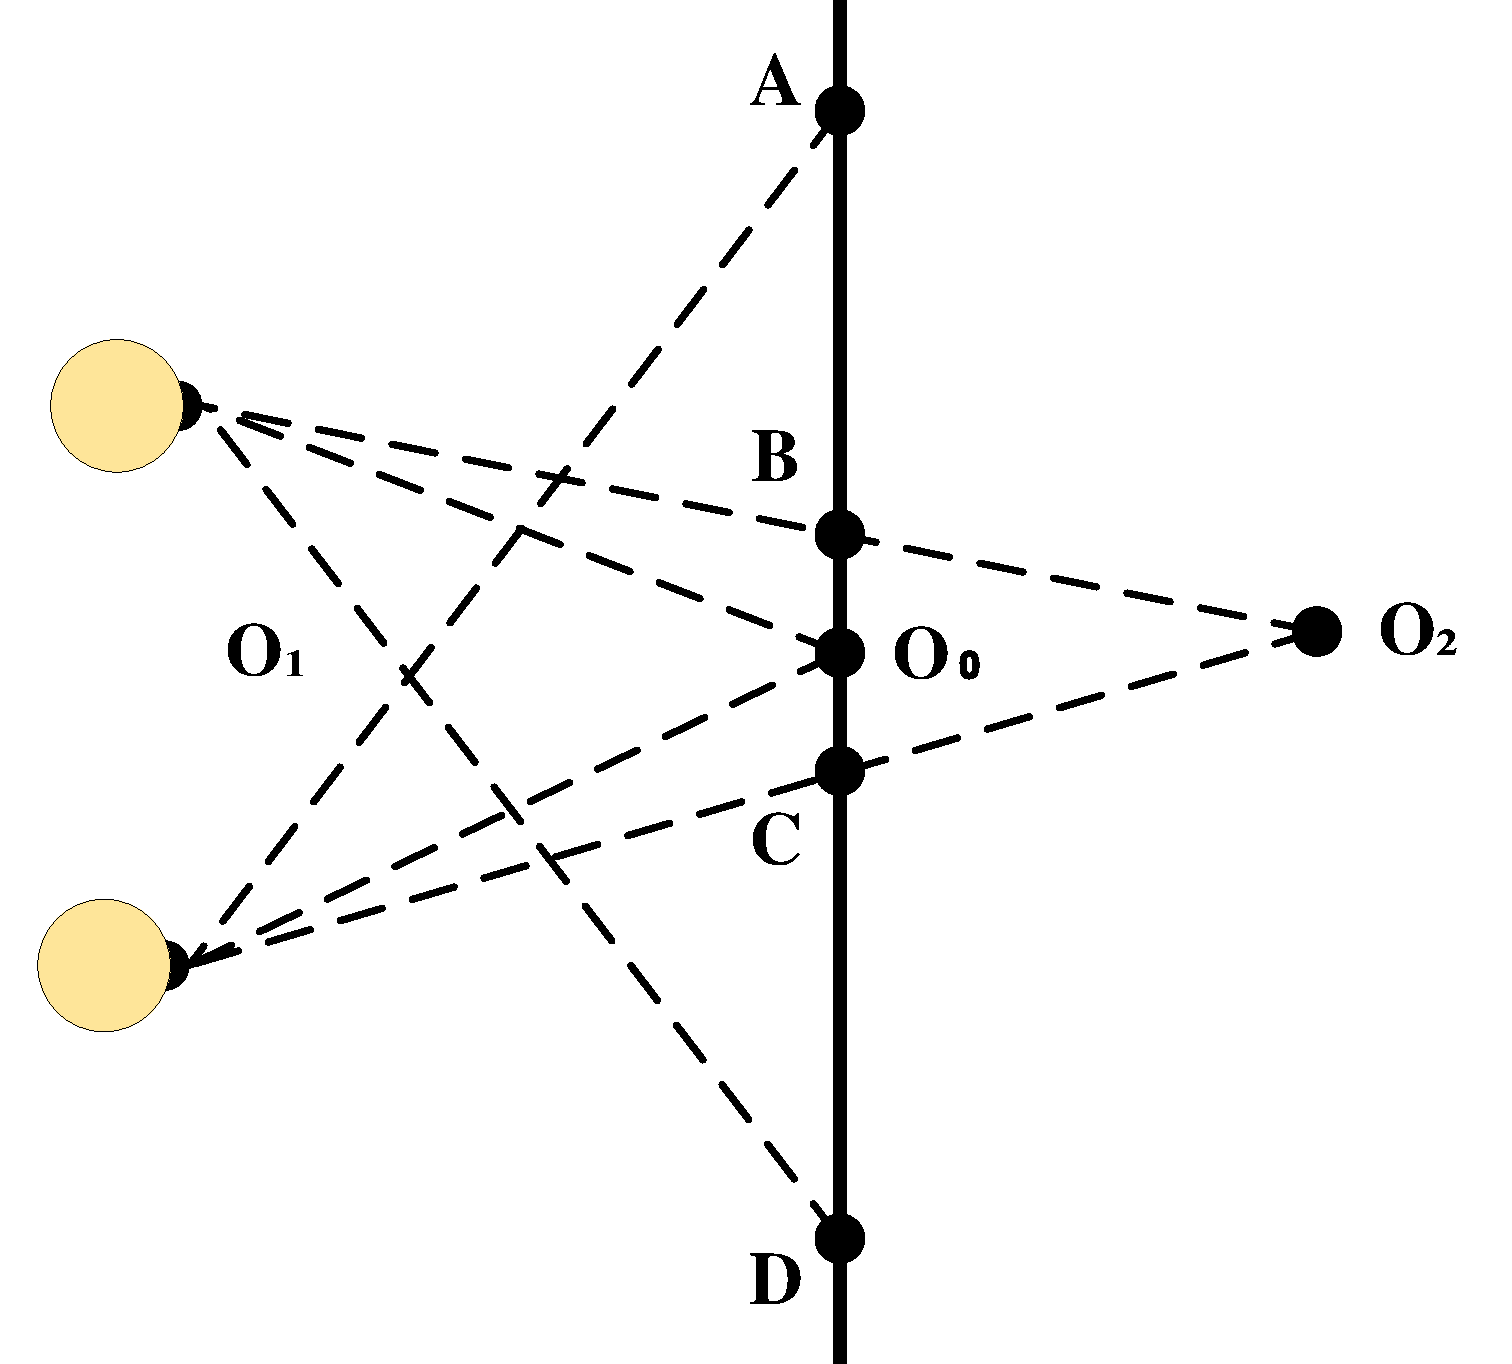
\includegraphics[width=0.5\textwidth]{resources/2p/2-3.pdf}
  % \bicaption{中文标题}{English Caption} % 使用中英文标题
  \caption{显示景深与视差的关系} % 只使用中文标题
  \label{fig:2-3}
  %\vspace{1 cm} % 使用该指令调整上下间距
\end{figure}

图\ref{fig:2-3}给出了景深感知与视差符号的对应关系\cite{Yamamoto2010}：目标位于零视差面时被感知在屏幕平面；当左右眼成像对应 B、C 时，目标 O$_1$ 呈“出屏”效果（正视差）；对应 A、D 时，目标 O$_2$ 呈“入屏”效果（负视差）。据此调节子像素排布和视差量，可在保证舒适性的同时扩展可感知深度范围\cite{Lee2015}。

\subsection{光场显示基础}
除数学定义外，光场模型在工程中还承担“表示接口”的角色：采集系统输出的数据格式、重建网络的输入组织方式以及显示系统的视点编码，通常都依赖同一套参数化约定。换言之，模型选择不仅决定理论表达能力，也直接影响软硬件协同效率。
光场模型用于统一描述空间中全部可见光线及其辐射属性，参数通常包含位置、方向、波长和时间\cite{Levoy2006}。通过该参数化形式，可在采集后进行重建与再渲染。与仅记录颜色强度的二维图像不同，光场数据天然携带角度信息，因此支持后聚焦、视点迁移和遮挡恢复等操作，这些能力对于人脸细粒度光照编辑尤为关键。
1936 年 Gershun 首次提出光场概念\cite{Gershun1936}，1991 年 Adelson 团队进一步给出七维全光函数的形式化表达\cite{Adelson1991}。图\ref{fig:2-4}(a)展示了其参数结构，对应数学式见公式\ref{eq:2-1}：


\begin{equation}
\label{eq:2-1}
I = L(x, y, z; \theta, \varphi, \lambda; t)
\end{equation}

在该表达中，$L$ 表示辐射亮度，$(x,y,z)$ 描述空间位置，$(\theta,\phi)$ 给出方向，$\lambda$ 与 $t$ 分别对应光谱和时间。其物理含义完整，但维度过高，直接用于动态场景采集与重建会显著增加存储与计算负担\cite{Ng2005}。

\begin{figure}[htbp]
  \centering
  % 第一张子图（左侧）
  \begin{minipage}{0.48\textwidth}  % 宽度减半，为左右排列留出空间
    \centering
    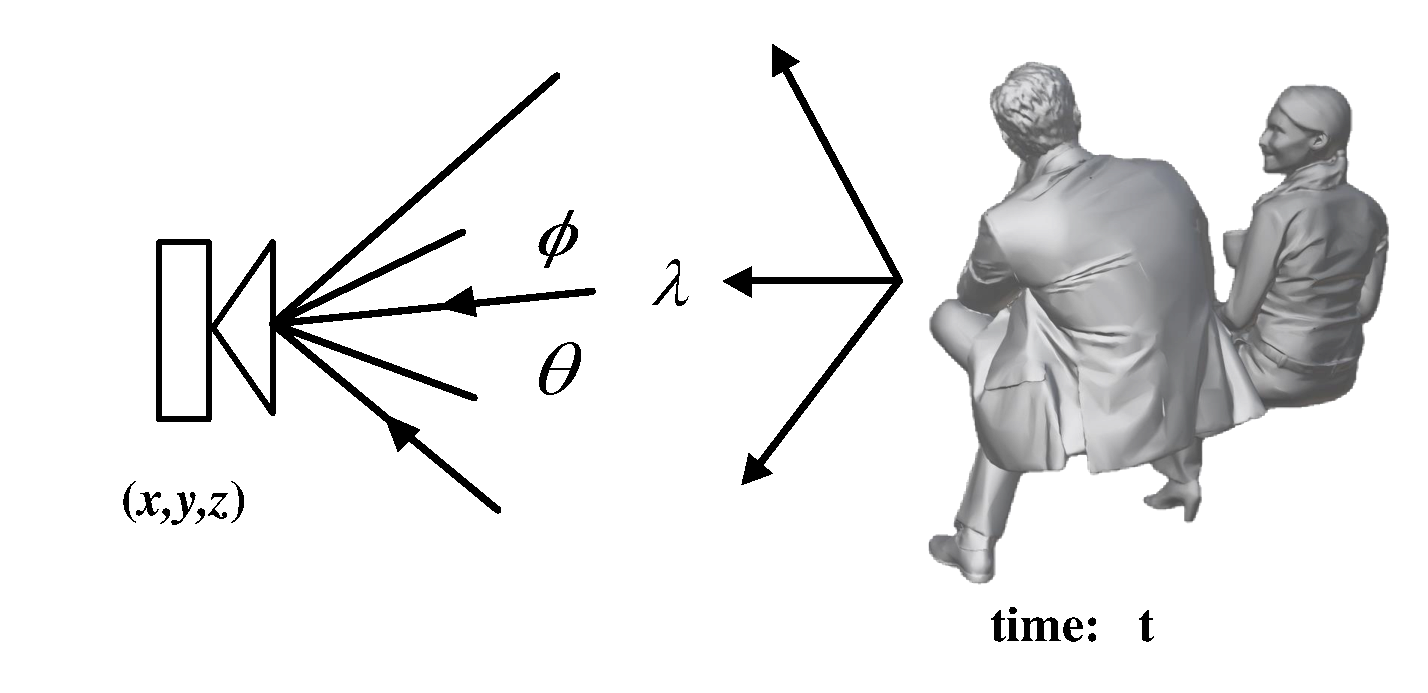
\includegraphics[width=0.9\linewidth, height=4cm]{resources/2p/2-4a.pdf}
    
    \centering\small(a) 
    \label{fig:2-4a}
  \end{minipage}
  \hfill  % 关键：添加水平间距，让两张图左右分开
  % 第二张子图（右侧）
  \begin{minipage}{0.48\textwidth}
    \centering
    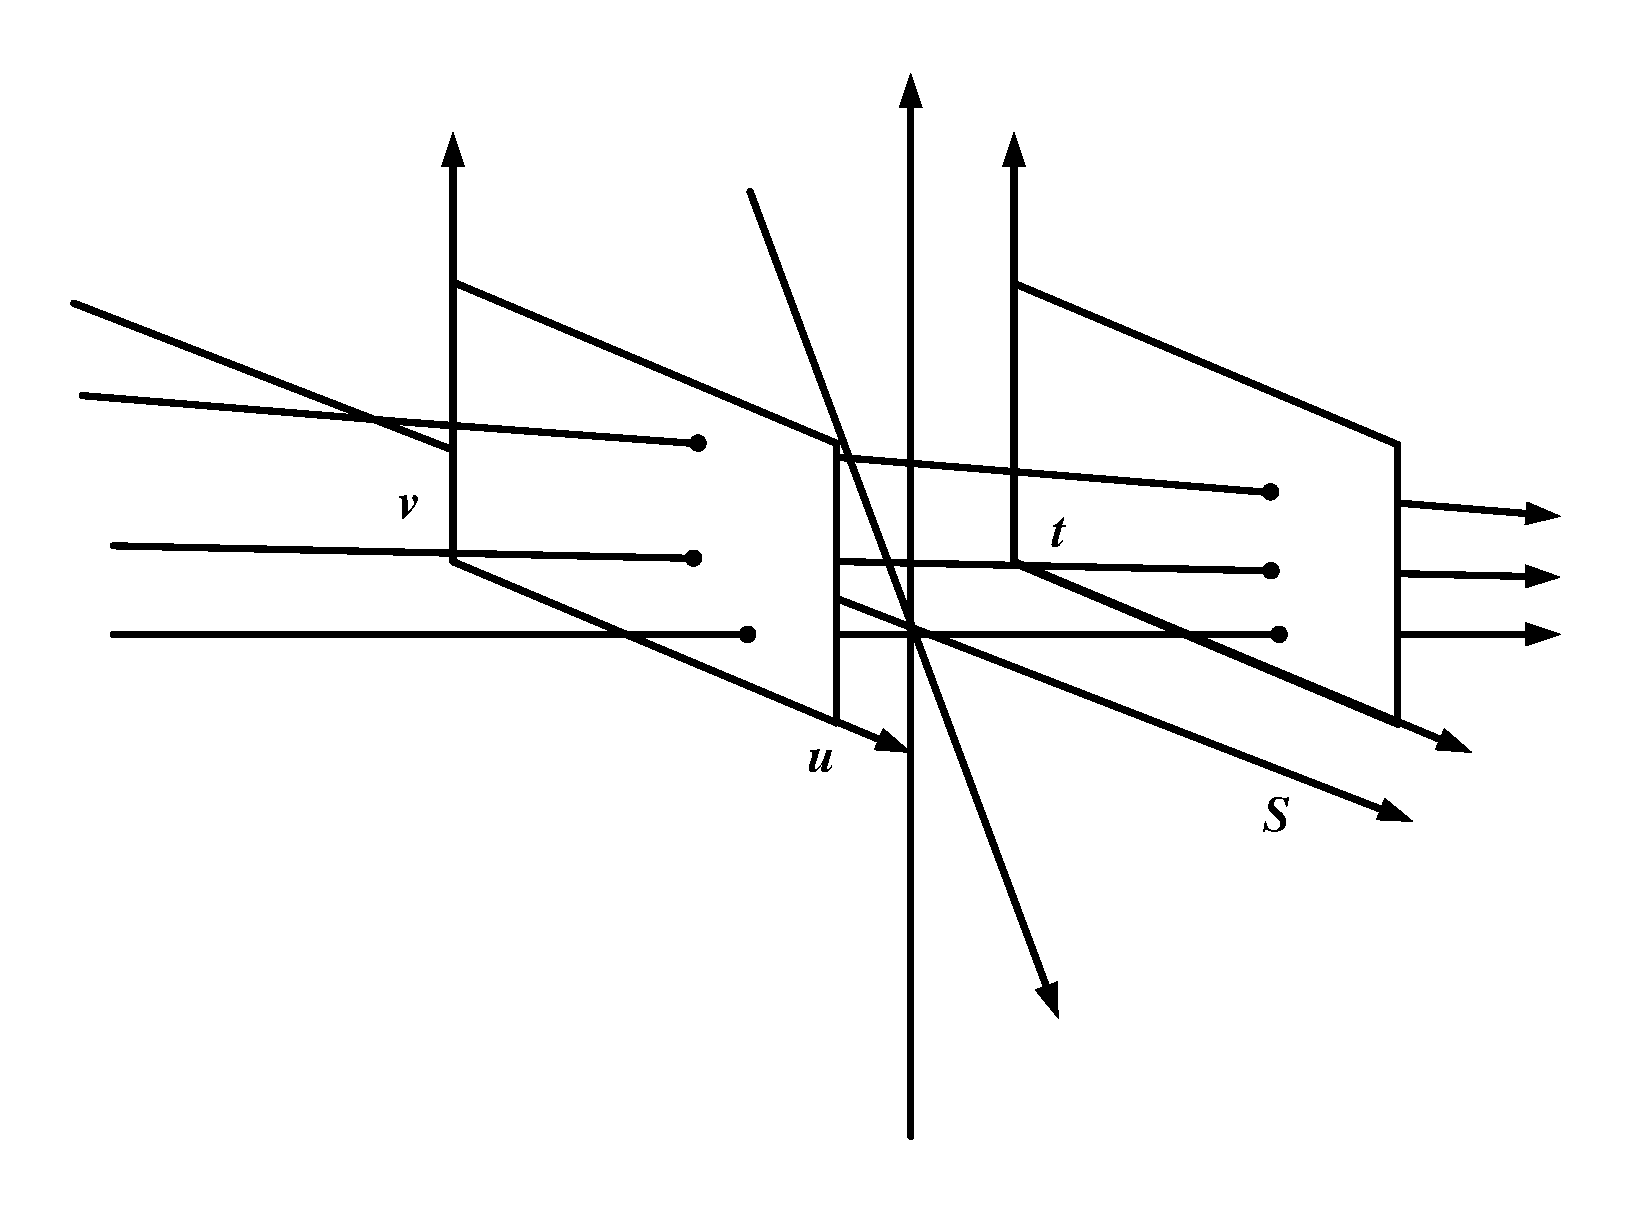
\includegraphics[width=0.9\linewidth, height=4cm]{resources/2p/2-4b.pdf}
    
    \centering\small(b) 
    \label{fig:2-4b}
  \end{minipage}

  % 大图标题：保持不变
  \caption{ (a)七维全光函数数学模型 (b)四维全光函数数学模型}
  \label{fig:2-4}
\end{figure}

为满足工程应用，通常先固定波长与时间维度，将全光函数从七维降至五维。进一步地，Levoy 团队提出双平面参数化（四维光场）\cite{Levoy1996}：用光线与两平行平面 $(s,t)$、$(u,v)$ 的交点唯一表示光线。图\ref{fig:2-4}(b)为其示意，数学形式如\ref{eq:2-2}。
% 独立公式优化版（变量用斜体，保持一致性）
\begin{equation}
\label{eq:2-2}
L = L(s, t, u, v) 
\end{equation}

其中 $(s,t)$ 与 $(u,v)$ 分别对应两平面交点坐标。该表示对少量特殊方向光线的刻画能力有限，但对人眼主要可见光线已足够完整；同时它显著降低了数据规模与重建复杂度，因此成为光场显示与渲染中的主流建模方式\cite{Ng2006}。在实际系统中，四维参数化还能与相机阵列或子孔径图像自然对接，便于后续完成视图插值、深度估计和光照一致性优化。




% 式中：
% \begin{itemize}
%   \item $I$ —— 光场的辐射强度（Intensity）；
%   \item $L$ —— 光场的辐射亮度（Radiance），是光场的核心物理量；
%   \item $(x, y, z)$ —— 三维空间中光线采样点的位置坐标；
%   \item $\theta, \varphi$ —— 光线传播的方位角和俯仰角，表征光线的传播方向；
%   \item $\lambda$ —— 光的光谱波长，决定光的颜色特性；
%   \item $t$ —— 时间维度，用于描述动态光场的变化过程。
% \end{itemize}

\subsection{基于光栅的光场显示器}

在多种光场显示方案中，水平视差柱镜光栅因结构成熟、光利用率高而应用广泛。该技术通过柱面透镜阵列对像素光线进行角度重分配，核心设计变量包括透镜曲率、焦距与排布周期。如图\ref{fig:2-5}(a)(b)所示，LCD 发出的子像素光经柱镜折射后被送往不同观察方向，从而输出多视点图像。与全视差系统相比，水平视差方案牺牲了垂直视差信息，但显著降低视点数量需求，使单视点可获得更高有效分辨率。典型硬件由 LCD、背光、功能膜层和柱镜光栅构成，其中功能膜层可通过调节扩散角提升视点均匀性。

\begin{figure}[htbp]
  \centering
  % 第一张子图（左侧）
  \begin{minipage}{0.48\textwidth}  % 宽度减半，为左右排列留出空间
    \centering
    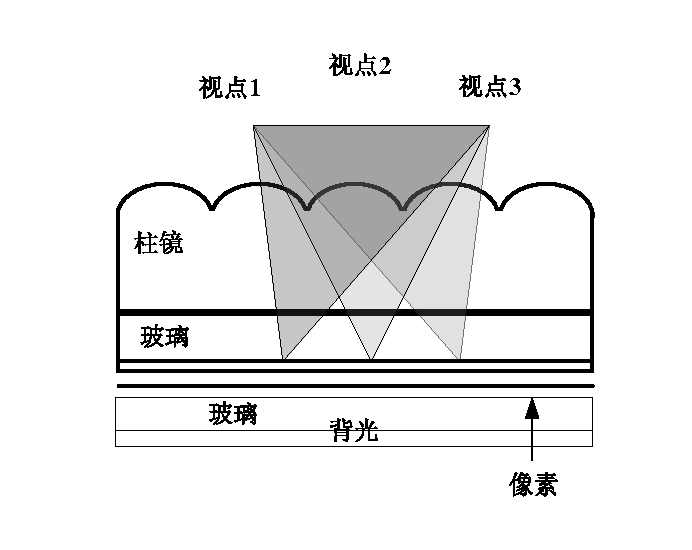
\includegraphics[width=0.9\linewidth, height=6cm]{resources/2p/2-5a.pdf}
    
    \centering\small(a) 
    \label{fig:2-5a}
  \end{minipage}
  \hfill  % 关键：添加水平间距，让两张图左右分开
  % 第二张子图（右侧）
  \begin{minipage}{0.48\textwidth}
    \centering
    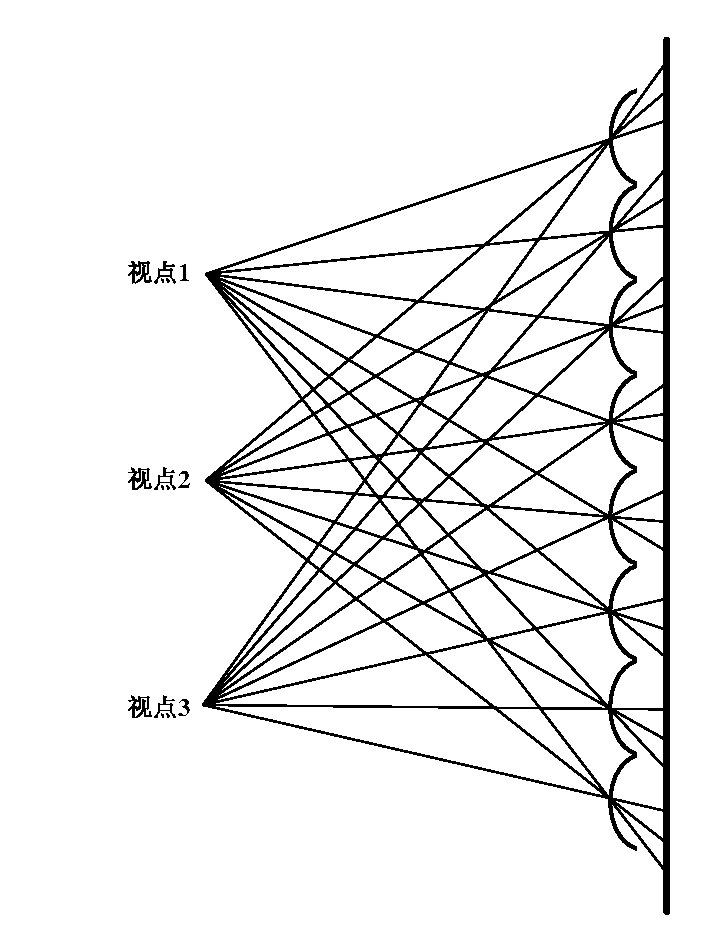
\includegraphics[width=0.9\linewidth, height=6cm]{resources/2p/2-5b.pdf}
    
    \centering\small(b) 
    \label{fig:2-5b}
  \end{minipage}

  % 大图标题：保持不变
  \caption{ (a)柱镜光栅显示器核心组件构成 (b)多视点排列特征及其空间分布规律可视化}
  \label{fig:2-5}
\end{figure}

在具体实现中，显示系统还要兼顾人因约束与硬件约束：人因层面关注观看距离、头部运动范围与视觉舒适阈值，硬件层面关注面板分辨率、透镜加工误差与亮度损失。两类约束共同决定可用视点数量和有效景深窗口。若系统仅追求视点密度而忽略亮度与串扰控制，实际观感反而可能下降。
柱镜的本质作用是把“像素位置”转换成“出射方向”。当 LCD 与柱镜焦面满足共轭关系后，原本发散的子像素光会被重整并沿特定角度传播，使不同像素组分别对应不同视点，实现方向编码。

\begin{figure}[H]
  \centering
  %\vspace{1 cm} % 使用该指令调整上下间距
  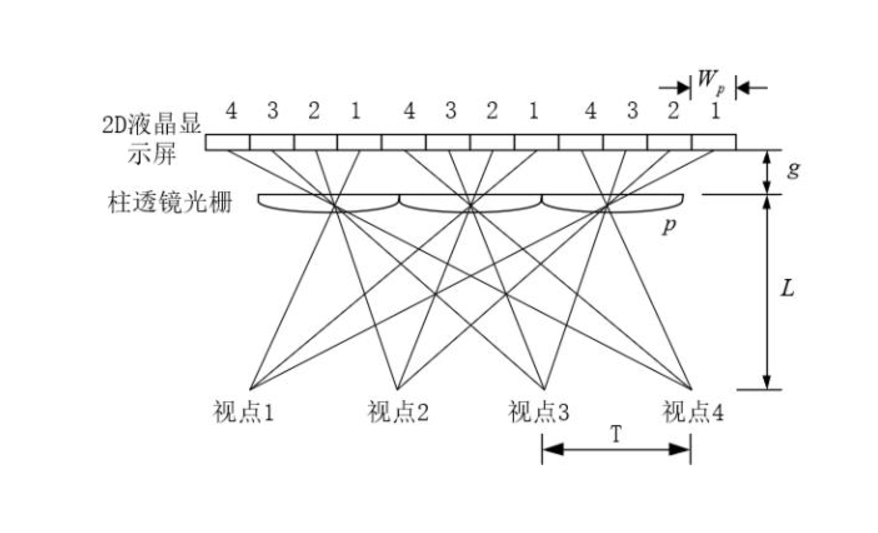
\includegraphics[width=0.8\textwidth,height=6cm]{resources/2p/2-6.pdf}
  % \bicaption{中文标题}{English Caption} % 使用中英文标题
  \caption{柱透镜覆盖子像素原理图} % 只使用中文标题
  \label{fig:2-6}
  %\vspace{1 cm} % 使用该指令调整上下间距
\end{figure}

如图\ref{fig:2-6}所示，当一个柱镜周期覆盖 4 个 LCD 子像素时，系统可形成 $N=4$ 个主视点方向。设计中需要联合优化透镜节距 $p$、曲率半径 $r$、面板间距 $g$、子像素宽度 $W_p$、最佳视距 $L$ 与视点间距 $T$。这些参数满足几何光学关系，可由相似三角推导得到：

\begin{equation}
T = \frac{L}{g} W_p \
\end{equation}

\begin{equation}
\frac{p}{N \cdot W_p} = \frac{L}{g + L} \
\end{equation}

由于柱镜与像素阵列均具周期结构，显示中容易出现摩尔纹和色散伪影。工程实现常将柱镜相对像素栅格倾斜约 $15^\circ$--$20^\circ$（常见取值约 $18^\circ$）以破坏周期共振并抑制干涉纹；再结合像素级或子像素级视点编码，可提升视点过渡连续性与观看稳定性。

\section{三维人脸光照编辑相关物理模型与评价指标}

光场人像编辑并非单一网络即可完成，其效果取决于成像几何、照明表达与渲染求解三部分的协同。为此，本节按“相机模型—光照模型—渲染模型”的顺序展开，分别说明数据从三维空间到二维图像的投影规则、环境光的参数化方式以及外观合成机制，为后续算法设计提供统一物理语境。需要强调的是，三类模型在训练与推理阶段常以“弱耦合、强约束”的方式交互：几何误差会传递到光照估计，光照偏差又会影响渲染一致性，因此评价环节必须同时观察多个维度。

\subsection{相机模型}
相机模型描述了三维点到二维像素的映射链路，如图\ref{fig:2-7}所示：

\begin{figure}[htbp]
  \centering
  %\vspace{1 cm} % 使用该指令调整上下间距
  
\includegraphics[width=0.8\textwidth,height=2cm]{resources/2p/2-7.pdf}
  % \bicaption{中文标题}{English Caption} % 使用中英文标题
  \caption{物体成像的过程} % 只使用中文标题
  \label{fig:2-7}
  %\vspace{1 cm} % 使用该指令调整上下间距
\end{figure}

相机投影过程可表示为：
\begin{equation}
q = \prod (Rp + t) \
\end{equation}
其中 $R,t$ 组成外参，用于将世界坐标下的点 $p$ 变换到相机坐标系得到 $p'$；符号 $\prod$ 表示投影算子（可对应透视或正交形式），再结合像素采样关系得到最终像素坐标 $q$。

在参数估计实践中，内参与外参通常通过标定板或多视图自标定联合获得。对于人脸视频序列，还需考虑轻微滚动快门、镜头畸变与面部非刚性运动带来的偏差。若这些因素未被建模，投影误差会在训练过程中被网络“错误吸收”，表现为几何漂移或局部纹理拉伸。因此，后续方法中会将基础标定结果与学习式微调结合，以提高整体鲁棒性。

在人脸重建与跟踪任务中，弱透视模型因参数少、求解稳定而常被采用，其表达式为：
\begin{equation}
u = s \cdot (x \cdot f / Z_0 + c_x), \quad v = s \cdot (y \cdot f / Z_0 + c_y) \
\end{equation}
其中 $(x,y,Z_0)$ 为相机坐标系点位，$f$ 为焦距，$Z_0$ 为目标平均深度，$s$ 为整体尺度，$(c_x,c_y)$ 为主点坐标，$(u,v)$ 为输出像素位置。

由于该模型计算代价低，常用于 2D 关键点与稠密配准流程\(^{[85]}\)。对应投影矩阵为：
\begin{equation}
\Pi = s
\begin{pmatrix}
1 & 0 & 0 \\
0 & 1 & 0
\end{pmatrix}
\end{equation}
其中 \(s = 1/d\) 为相似缩放因子，\(d\) 代表平均深度，反映“距离变化导致成像尺度变化”的规律。实际训练时，常将 3D 预测结果投影到 2D，与标注图像比较后构建损失函数。若结合多视图监督，还可额外引入跨视点重投影一致性项，以提升几何稳健性并抑制局部漂移。
\subsection{光照模型}


% 正文内容
光照建模是实现真实感外观的核心难点。传统 Lambert、Phong、Blinn--Phong 等局部模型通常只考虑有限光源，难以完整覆盖环境光、多次反射和间接照明效应\cite{Phong1975,Blinn1977}。随着 HDR 环境贴图与全局照明方法的发展\cite{Debevec1997}，光照表示逐渐转向球面函数框架，即把入射光分布视为单位球面上的连续函数\cite{Ramamoorthi2001}。对于人脸场景而言，这一点尤其重要：皮肤、头发和眼部区域在同一光照下会呈现明显不同的反射特性，低阶模型若表达不足，往往会出现“整体亮度对了但质感失真”的问题。

球谐函数可看作球面傅里叶基，具备正交、完备和良好旋转性质\cite{Morse1953}，因此非常适合低频光照压缩。在实时渲染、PRT\cite{Sloan2002}、三维重建及 NeRF 光照分解等场景中，它已成为基础表示。其定义如下。

在三维欧氏空间中，任一方向向量 $w$ 可通过球坐标表示为：
\begin{equation}  % 替换\[...\]为equation环境，自动编号
w = (\theta, \phi)
\label{eq:2-8}
\end{equation}

其中 $\theta$ 为极角，$\phi$ 为方位角。复数形式球谐函数定义为：
\begin{equation}
Y_l^m(\theta, \phi) = N_l^m P_l^m(\cos \theta) e^{im\phi}
\end{equation}

其中，$l$ 为阶数，$m$ 为次数，$P_l^m$ 为带勒让德多项式，$N_l^m$ 为归一化因子，具体如下：
\begin{equation}
N_l^m = \sqrt{\frac{(2l+1)(l-m)!}{4\pi(l+m)!}}
\end{equation}

在图形学实现中，通常采用实数球谐函数以规避复数运算，实数球谐函数表达式为：
\begin{equation}
Y_l^{m} =
\begin{cases}
\sqrt{2}N_l^{m}\cos(m\phi)P_l^{m}(\cos\theta), & m > 0 \\
N_l^{0}P_l^{0}(\cos\theta), & m = 0 \\
\sqrt{2}N_l^{|m|}\sin(|m|\phi)P_l^{|m|}(\cos\theta), & m < 0
\end{cases}
\end{equation}

通过球谐展开可得到如下表达式：
\begin{equation}
f(w) = \sum_{l=0}^{\infty} \sum_{m=-l}^{l} c_l^m Y_l^m(w)
\end{equation}

其中：
\begin{equation}
c_l^m = \int_{S^2} f(w) Y_l^m(w) dw
\end{equation}

球谐系数可理解为光照在不同角频率上的能量投影：$l=0$ 近似整体亮度，$l=1$ 刻画主照明方向，$l=2$ 主要反映软阴影与低频遮挡；更高阶用于表达高光与锐利阴影。阶数提升会改善细节，但参数量与计算量约按 $O(l^2)$ 增长。

基于球谐函数的光照模型的环境光照表示如下：
\begin{equation}
L(w) \approx \sum_{i=1}^{n} c_i Y_i(w)
\end{equation}

工程实践中常采用三阶 SH（9 个系数）在效率与质量间折中。Lambert 漫反射积分可写为：
\begin{equation}
I(n) = \int_{S^2} L(w) \max(0, n \cdot w) dw
\end{equation}

做球谐卷积近似后可得：
\begin{equation}
I(n) \approx \sum_{i=1}^{9} c_i k_i(n)
\end{equation}

其中 $k_i(n)$ 是与法线方向相关的卷积核项。已有研究表明，Lambert 项通常用二阶 SH 即可达到较好近似精度。

图\ref{fig:2-8}展示了球谐基函数形态。凭借低频表达高效、旋转处理方便等特点，SH 已成为实时渲染与重建系统中的常用组件\cite{Green2003,Kautz2004}；在可微渲染与神经场方法中，它同样被广泛用于光照学习与可编辑表示\cite{Li2020,Martin-Brualla2021}。

\begin{figure}[htbp]
  \centering
  %\vspace{1 cm} % 使用该指令调整上下间距
  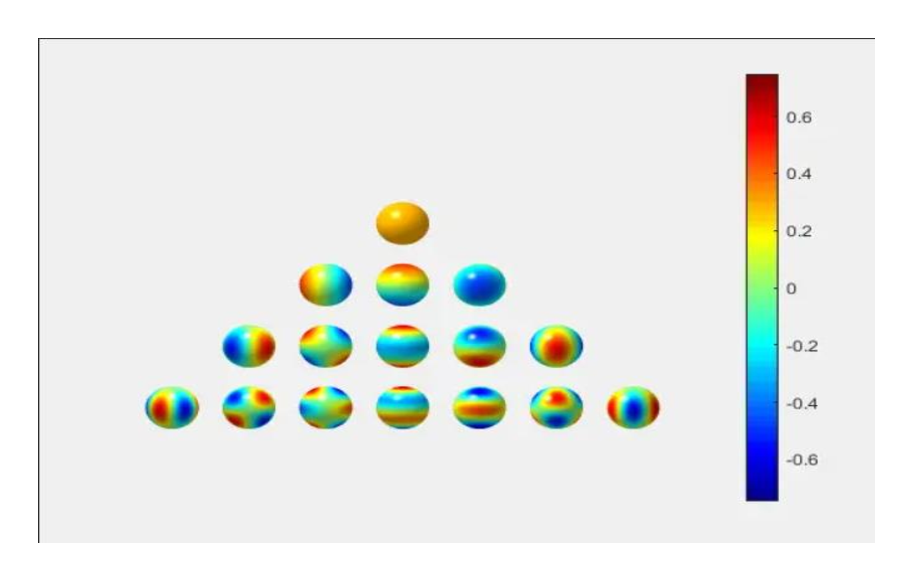
\includegraphics[width=0.8\textwidth,height=8cm]{resources/2p/2-8.pdf}
  % \bicaption{中文标题}{English Caption} % 使用中英文标题
  \caption{球谐函数可视化} % 只使用中文标题
  \label{fig:2-8}
  %\vspace{1 cm} % 使用该指令调整上下间距
\end{figure}

\subsection{渲染模型}
渲染模型在本研究中的作用可概括为“把可估计的物理量转成可感知的视觉结果”。当几何、材质与光照参数发生微小变化时，渲染器需要给出稳定且可解释的像素响应，这一点对光照编辑尤为关键。若渲染过程不稳定，即便网络在训练集上收敛，也容易在跨视角浏览时出现闪烁、明暗漂移或局部伪影。

（1）传统渲染模型
在离线内容生产中，传统渲染管线仍具有不可替代的价值：一方面，材质和灯光参数具备明确物理含义，便于艺术家精细调参；另一方面，成熟的软件生态提供了可靠的资产管理与流程复用能力。对于论文实验而言，传统渲染结果也常被用作对照基准，以评估神经方法在真实感与泛化能力上的增益。

传统渲染模型的核心是依托计算机图形学渲染管线，将三维虚拟几何模型生成具有连续观看效果且真实感较强的三维光场图像。这里的虚拟几何模型通常是人工构建的仿真模型，包含材质和纹理属性。制作者一般使用三维建模软件（如 Blender、3ds Max 等）完成目标建模\cite{BlenderFoundation2019}，在制作阶段通常不直接使用真实场景采集的图像或深度信息。

基于虚拟几何模型的光场内容生成流程通常包括光照模型配置、几何模型布置、纹理与材质映射以及光场编码等环节。早期图形学渲染方法主要依赖光栅化（Rasterization）路径，利用顶点、线段与面片表征虚拟几何模型，并通过纹理映射补充颜色细节。该阶段的光照建模以基础模型为主，例如朗伯光照模型（Lambert's Model）用于刻画漫反射过程，菲涅尔方程（Fresnel equations）用于描述光线在不同介质间的反射和折射\cite{Born1999}。由于难以准确模拟全局光照，早期渲染效果普遍真实性不足。

随着 GPU 计算能力提升与人工建模技术持续优化，基于虚拟几何模型的三维光场内容生成进入新阶段。受益于更高计算效率，面向三维光场的渲染方法在保证一定帧率的同时能够纳入更多提升观看体验的因素，包括更精确的物理渲染机制与更复杂的光照模型以逼近真实场景。在这一背景下，多种可生成更真实光场内容的渲染方法相继提出，并在部分场景实现了实时渲染。

例如，光线追踪技术（Ray Tracing）通过模拟虚拟光线在仿真场景中的传播和虚拟几何模型的交互过程，对光线的反射、折射和阴影等现象进行更为精细的描述\cite{Pharr2016}。基于英伟达的CUDA框架，研究者对投射光线进行并行计算，显著提高了虚拟视点的生成速度，在某些条件下使得基于虚拟几何的三维光场内容生成速度达到了实时。此外，基于蒙特卡洛路径追踪（Monte Carlo Path Tracing）的渲染方法通过对光线的随机采样策略提升了渲染效率。更进一步，基于物理的渲染（Physically Based Rendering, PBR）方法通过双向反射分布函数（Bidirectional Reflectance Distribution Function, BRDF）模拟具有不同材质特性的虚拟几何模型表面特性\cite{Walter2007}。PBR方法统计了不同角度的输入光，在漫反射和高光反射下的光线输出，从而基于物理规律对光线的入射和反射过程进行建模。其反射率方程为：
\begin{equation}
L_o(w_o, x) = \int_{\Omega} f_{brdf}(w_o, w_i, x) \cdot L_i(w_i, x) \cdot (w_i \cdot n) dw_i
\end{equation}

其中，$x$ 表示模型表面被入射光线集中的位置，$w_i$ 表示在半球面范围内入射光线的方向，$w_o$ 为出射光线的方向，$n$ 为模型表面在 $x$ 点的法向量，$L_i$ 是入射光线的辐照度，其包含局部和全局光照，$L_o$ 是出射光线的辐照度。$f_{brdf}$ 为半球面上的BRDF函数，其中包含了对漫反射和高光（镜面）反射的建模，可表示为：
\begin{equation}
f_{brdf} = f_d + f_s = \frac{1 - m}{\pi} \cdot b + \frac{D(h; r, b, m) \cdot F(v, h; b, m) \cdot G(w_i, w_o, h; r)}{(n \cdot w_i) \cdot (n \cdot w_o)}
\end{equation}

其中，$f_d$ 表示漫反射过程，$f_s$ 表示高光反射过程。$m$ 表示金属度，$r$ 表示粗糙度，$b$ 表示基础颜色，$D$ 为法向量项，$F$ 为菲涅尔项，$G$ 为几何项。此外，环境光遮蔽（Ambient Occlusion, AO）的进一步引入能够更加精确地计算出间接光照，同时结合全局光照（Global Illumination, GI）使渲染效果更加贴近真实场景。PBR方法的光照过程不仅考虑了光线在物体表面间的多次光照反射，这使得光照计算不再局限于直接光照，还能够模拟间接光源带来的真实效果。同时，还可基于深度学习对所渲染的画面进行降噪处理。但令人遗憾的是，这种传统渲染模型生成三维光场内容的方式存在很大的不足，比如人工制作的虚拟几何模型本身就缺乏真实物品特有的细节。且在建模的过程中，往往需要依赖复杂的材质及光照设计等手段来弥补渲染过程缺乏的真实感。因此在进行虚拟模型设计及动态模型的制作时往往需要较高的成本。
\subsubsection{基于Nerf的体渲染模型}
神经辐射场技术目前已在三维重建与多视点生成等方向广泛应用，也常被视作新型渲染方法。在利用 NeRF 生成三维光场内容前，需先对目标场景进行稀疏采集，并基于不同视角拍摄的 RGB 图像完成相机内参与外参标定，具体可采用 COLMAP 工具。

\begin{figure}[htbp]
  \centering
  %\vspace{1 cm} % 使用该指令调整上下间距
  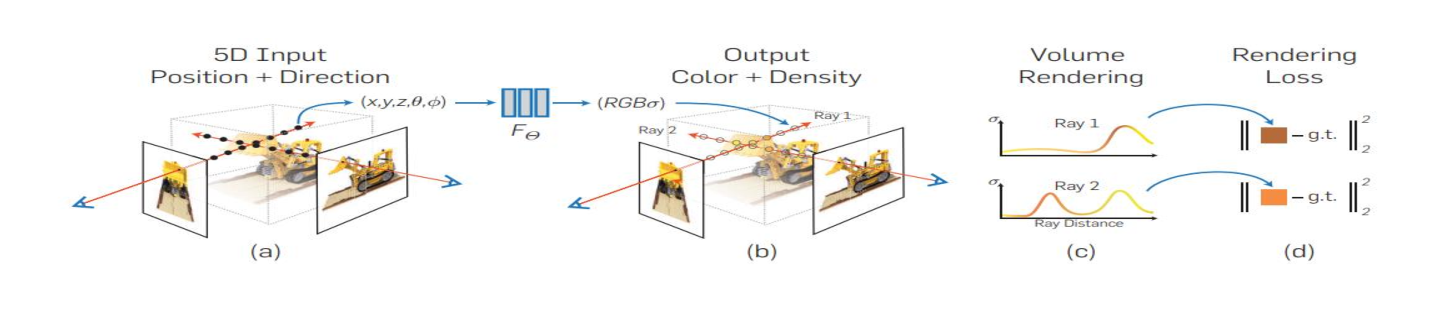
\includegraphics[width=0.9\textwidth,height=4cm]{resources/2p/2-9.pdf}
  % \bicaption{中文标题}{English Caption} % 使用中英文标题
  \caption{Nerf体渲染模型} % 只使用中文标题
  \label{fig:2-9}
  %\vspace{1 cm} % 使用该指令调整上下间距
\end{figure}

NeRF 的整体流程如图\ref{fig:2-9}所示。在训练过程中，NeRF 首先根据求得的相机位姿计算出用于训练的图片中每个像素所对应的渲染光线，其中每条光线可表示为：
\begin{equation}
r(t) = o + td
\end{equation}

其中，$o$ 为对应图像的相机原点，$d$ 为方向向量，$t$ 为光线传播的距离。接下来是第一轮粗采样过程。每个待计算颜色的像素均投射出一根渲染光线并在该光线上进行均匀采样，得到 $N_c$ 个采样点。其中每个采样点 $(x, y, z, \theta, \phi)$ 用其位置 $(x, y, z)$ 和所在射线的方向向量 $(\theta, \phi)$ 共同定义。下一步，NeRF 对输入的采样点进行正余弦位置编码，用于扩充采样点的高频分量，提升神经网络对场景细节的表达能力。其位置编码函数如下：
\begin{equation}
\gamma(p) = \left(\sin(2^0 \pi p), \cos(2^0 \pi p), \dots, \sin(2^{L-1} \pi p), \cos(2^{L-1} \pi p)\right)
\end{equation}

其中 $L$ 为数据扩充的维度参数，对于输入的位置向量，$L$ 的值为 10，对于方向向量，$L$ 的值为 4。之后，将得到的编码向量输入至多层感知机（MLP）神经网络 $F$，用于估计出每个采样点的颜色值和点密度 $\sigma$。其中点密度的估计只与位置向量相关，而颜色值的估计会同时依赖于输入的位置和方向向量。由此可得每个采样点所对应的权重可表示为：
\begin{equation}
w_i = T_i \cdot (1 - \exp(-\sigma_i \delta_i))
\end{equation}

此外，NeRF 使用了重采样策略，根据第一轮粗采样点的位置和权重 $w_i$，通过计算概率密度函数（Probability Density Function, PDF）进行第二轮重要性采样，选取的采样点个数为 $N_f$。之后将第二轮和第一轮的采样点一同输入到第二阶段的神经网络中，预测所有采样点的颜色和点密度值。为了计算图像中每个像素点的颜色，NeRF 方法基于体渲染（Volume Rendering）技术沿着渲染光线传播的方向统计光线上的所有采样点，并用离散化求和的操作来近似连续区域的积分，从而估计每个像素点的颜色。此过程可表示为：
\begin{equation}
\hat{C}(r) = \sum_{i=1}^{N} T_i \cdot (1 - \exp(-\sigma_i \delta_i)) \cdot c_i
\end{equation}

其中，$i \in [1, N]$ 为一条光线上的采样点个数，$\delta_i = t_{i+1} - t_i$ 为第 $i$ 个采样点的线段长度，$c_i$ 为每个采样点的颜色，$T_i$ 表示累积到第 $i$ 个采样点之前的剩余可见度，$\hat{C}$ 为渲染光线所对应的像素颜色。对于优化 NeRF 神经网络的误差函数，NeRF 对预测的颜色 $\hat{C}$ 和对应的真实颜色计算平方误差，定义为：
\begin{equation}
L = \sum_{r \in \mathcal{R}} \left\|\hat{C}(r) - C(r)\right\|_2^2
\end{equation}

网络训练完成后，NeRF 可在目标场景中任意设定观测位置与朝向，从而实现真实场景下的三维光场内容生成。与传统几何驱动方法相比，NeRF 的优势在于对复杂外观细节具有更强拟合能力，尤其在毛发、半透明区域与软阴影边缘等位置表现更稳定；但其代价是训练与渲染开销较大，对数据采集质量也更敏感。因此，实际应用中常结合蒸馏、稀疏采样或网格-神经混合表示来平衡效率与质量。

此外，从系统工程角度看，三维光场人脸光照编辑还涉及数据链路闭环：采集端决定可恢复信息上限，表示端决定可学习结构，显示端决定最终观看体验。若三者在参数定义上不一致，即便单模块性能较高，也可能在端到端流程中出现误差累积。例如，采集时曝光策略与渲染时色彩空间不匹配，会导致光照编辑结果在不同设备上观感差异显著；又如，视点标定存在微小系统误差，可能在视频播放中被放大为轻微抖动。基于此，后续章节的方法设计将尽量采用可解释参数与统一坐标约定，并在训练阶段引入跨视角约束，以降低误差传递风险。
\subsection{图像评价指标}
评价体系不仅用于“给分”，更用于定位问题来源。例如，当 PSNR 提升而 LPIPS 无明显改善时，通常意味着像素误差下降但感知质量收益有限；当 ID 指标下降且 LE/LI 波动增大时，往往提示光照编辑破坏了身份一致性。基于这种诊断逻辑，可更有针对性地调整损失函数权重与训练采样策略。

在实验报告层面，本文也强调“定量结果+可视化现象”的联合呈现。对于光照编辑任务，单纯比较分数可能掩盖一些关键问题，例如高频高光区域局部过曝、边缘区域色偏或跨帧微闪烁等。这些问题不一定显著拉低某个单独指标，却会明显影响主观体验。因此，在后续章节中，除统一给出指标统计外，还会配合典型失败案例分析，说明方法在极端光照与大姿态条件下的行为边界。
为客观评估后续方法在图像质量、跨视角一致性和时间稳定性上的表现，本文构建了多维指标集合：质量指标 FID、PSNR、SSIM、LPIPS；多视角一致性指标 ID、LE、LI；时序指标 WE 与 Temporal LPIPS。各指标定义如下。需要指出，任何单一指标都难以完整反映“可编辑光场人像”的真实质量，因此本文采用组合评价策略：先用像素与感知指标衡量重建准确度，再用身份与时序指标验证编辑稳定性。

此外，在跨数据集比较时还应统一预处理协议，包括人脸对齐、分辨率归一化与掩码区域定义。若这些前处理不一致，指标差异可能主要来自数据管线而非模型本身，导致结论偏差。为避免该问题，本文后续实验将固定评测脚本与随机种子，并在附录给出关键参数。

FID 衡量生成样本分布与真实分布之间的统计距离，是生成任务中常用的感知指标。做法是用预训练 Inception 网络提取两组特征，再计算 Fr'echet 距离：
\begin{equation}
\text{FID} = \left\| \mu_r - \mu_g \right\|_2^2 + \text{Tr}\left( \Sigma_r + \Sigma_g - 2\left( \Sigma_r \Sigma_g \right)^{\frac{1}{2}} \right)
\end{equation}
其中 $\mu_r,\Sigma_r$ 与 $\mu_g,\Sigma_g$ 分别是两组特征的均值和协方差。FID 越小，说明生成分布越接近真实分布。

PSNR 用于刻画像素层面的重建误差，基于均方误差（MSE）定义如下：
\begin{equation}
\text{PSNR} = 10\log_{10} \frac{MAX^2}{MSE}
\end{equation}
其中 $MAX$ 为像素上限（常取 255）。PSNR 越高，表示像素重建误差越小。

SSIM 同时考虑亮度、对比度和结构一致性，表达式为：
\begin{equation}
\text{SSIM}(x, y) = \frac{(2u_x u_y + C_1)(2\sigma_{xy} + C_2)}{(u_x^2 + u_y^2 + C_1)(\sigma_x^2 + \sigma_y^2 + C_2)}
\end{equation}
其中 $u$ 为均值，$\sigma$ 为方差，$\sigma_{xy}$ 为协方差。指标越接近 1，结构相似性越高。

LPIPS 在深度特征空间中比较两幅图像的感知差异，更接近人眼主观判断；数值越小表示视觉上越相似。

ID 指标用于衡量不同视角下人物身份特征的一致性，通常通过人脸识别网络提取嵌入特征向量，并计算余弦相似度：
\begin{equation}
\text{ID} = \frac{f_1 \cdot f_2}{\left\| f_1 \right\| \left\| f_2 \right\|}
\end{equation}

ID 值越高，表示跨视角身份保持越稳定。

LE 衡量相邻帧光照参数或亮度统计的偏移量，值越小说明光照连续性越好。

LI 描述不同视角之间整体光照分布的不一致程度，通常由直方图差或光照方向误差计算，值越低越好。

WE 在光流对齐后计算相邻帧残差，可反映时序几何与纹理稳定性；指标越小越稳定。

Temporal LPIPS 将感知距离扩展到视频域，通过相邻帧特征差异评估闪烁与抖动；数值越低表示时序更平滑。这一点也说明，评价阶段应同时关注“是否逼真”与“是否稳定可控”，二者缺一不可。

从阅读与复现角度出发，本章还尽量统一符号约定和变量含义，减少跨小节理解成本。对同一概念若存在多种称谓，统一采用一次定义、后续复用的写法，以保证全文逻辑闭环。
\section{本章小结}
本章完成了三维光场人脸光照编辑的基础铺垫。首先，从心理与生理两类深度线索解释了立体视觉形成机制，并给出正负视差与景深感之间的对应关系，为后续视差与显示参数设计提供依据。其次，围绕光场建模路径，回顾了从七维全光函数到四维双平面参数化的降维思路，明确了工程可实现性与表达能力之间的平衡点；同时分析了柱镜光栅显示器的结构组成、关键几何参数和抗伪影策略。

在物理建模方面，本章进一步梳理了相机投影、球谐光照、传统 PBR 渲染与 NeRF 体渲染的核心流程，说明了它们在三维人脸外观重建与光照编辑中的功能分工。最后，建立了覆盖图像质量、多视角一致性和时序稳定性的评估指标集合，为后续章节的对比实验与消融分析提供统一度量标准。总体而言，本章给出的理论与模型构成了全文方法设计和实验验证的基础支撑。
为便于后续章节直接继承，本章术语使用尽量保持单义：例如将“光照一致性”限定为跨视角或跨时间的照明参数平稳性，将“身份一致性”限定为人脸语义特征保持，将“结构一致性”限定为几何轮廓与局部纹理关系不失真。这样的定义方式有助于把主观描述转换为可计算目标，避免出现“视觉上更好但无法量化解释”的问题。同时，本章在介绍模型时有意区分了“可解释模型”和“高拟合模型”的角色边界：前者提供可控参数与物理先验，后者负责补足复杂外观细节；二者结合能够在真实感、可控性和泛化性之间取得更稳妥平衡。最后，考虑到论文方法需要面对多设备、多场景与多光照条件，本章所建立的理论框架强调模块可替换性——在不改变整体评价协议的前提下，后续可将不同相机标定策略、不同光照表示或不同渲染后端接入同一流程进行公平比较，这也为后续实验扩展提供了方法学保障。
进一步地，本章也给出了一个可复用的方法学框架：以视觉感知约束定义“看起来自然”，以物理模型约束定义“生成过程合理”，再以多指标评测闭环验证“结果稳定可复现”。该框架既适用于本文任务，也可迁移到其他多视点人像编辑问题。




















%第二章
\chapter{关键信息驱动的三维光场静态人脸光照编辑}

近年来，三维光场技术取得显著进步，三维光场显示可以提供理想的立体视觉体验，观者在其中观看三维场景就像它们存在于真实空间一样。它能够提升虚拟现实等领域的用户体验，对于数字媒体和人机交互的发展起到重要影响。真实空间中，物体的明暗分布取决于光照，光照与阴影可以凸显画面的深度。而在三维光场显示中，光照同样是增加 3D 显示真实感和空间感的重要因素，通过编辑光照，可以大大提升立体显示效果。而合理准确的光照对于三维光场的显示效果起到非常关键的作用，光照编辑是三维光场中用于调整三维光场显示效果的常用方法。目前，对于三维光场人像光照编辑有两种方式。分别是多视图同时编辑方法和基于光照条件的密集视点采集方法。

对于多视图同时编辑方法，由于三维光场内容由多视图构成，不同视图间的光照信息相互关联，当单独处理某一单张视图的光照时，会使多视图之间的光照一致性得不到保证,进而削弱三维光场的真实感与连贯性。对于基于光照条件的密集视点采集方法，可以保证较好的多视图之间的光照一致性，但是需要搭建大规模数据采集设备。

为解决三维光场人像编辑中面临的数据采集复杂与光照一致性问题，本章提出了一种关键信息驱动的三维光场人像光照编辑方法，该方法通过抽取三维光场的多视图，获取漫反射分量，针对抽取的单张人像图像，采用高光去除算法对原始光照进行预处理，结合高光阈值多重判断来去除图像高光。从全景 HDR 图像中快速获取环境光信息并使用语义级别描述\cite{Dong2016,Sennrich2016,Vaswani2017}的对光照潜空间的关键信息进行编辑，获取关键光照信息(SH系数)\cite{Google2025,Ramamoorthi2001}
。最后进行重建，将图像解耦成几何空间和光照潜空间\cite{Jiang2023}，然后通过体渲染\cite{Mildenhall2022}渲染得到多视图，最后通过光场编码后在3D显示器上进行显示验证，完成对三维光场人像光照的编辑。通过实验对本方法进行了客观和主观评价，在多项指标上均优于先前的重光照方法，证明了该方法在提高了光照一致性的前提下，简单高效的实现了对三维光场人像光照的编辑。



\section{基本原理}
对于三维光场人像光照的编辑，常常使用多张视差图同时进行光照编辑的方法和基于光照条件的密集视点采集方法。前者方法虽然简单，但是在三维光场背景下却不再适用。三维光场内容由多视图构成，不同视图间的光照信息相互关联，当分别编辑某单张视图的光照时，会使得编辑后的多视图之间的光照一致性得不到保证，进而导致三维光场的真实感与连贯性降低。后者方法保证光照的一致性，通过搭建密集光场采集设备，同时部署多组可独立调控的 LED 光源，分布在相机阵列外围或顶部，形成自定义光照条件来拍摄得到多视图。但是密集视点采集方法需要搭建大规模数据采集设备。

基于上述背景，为解决三维光场人像光照编辑中的光照一致性不强和采集方法复杂的问题。本文提出了一种关键信息驱动的三维光场人像光照编辑方法，通过获取图像中的光照关键信息，在提高了光照一致性的前提下，简单高效的实现了对三维光场光照的编辑，完整的工作流程图如图\ref{fig:3-1}所示。

\begin{figure}[htbp]
  \centering
  %\vspace{1 cm} % 使用该指令调整上下间距
  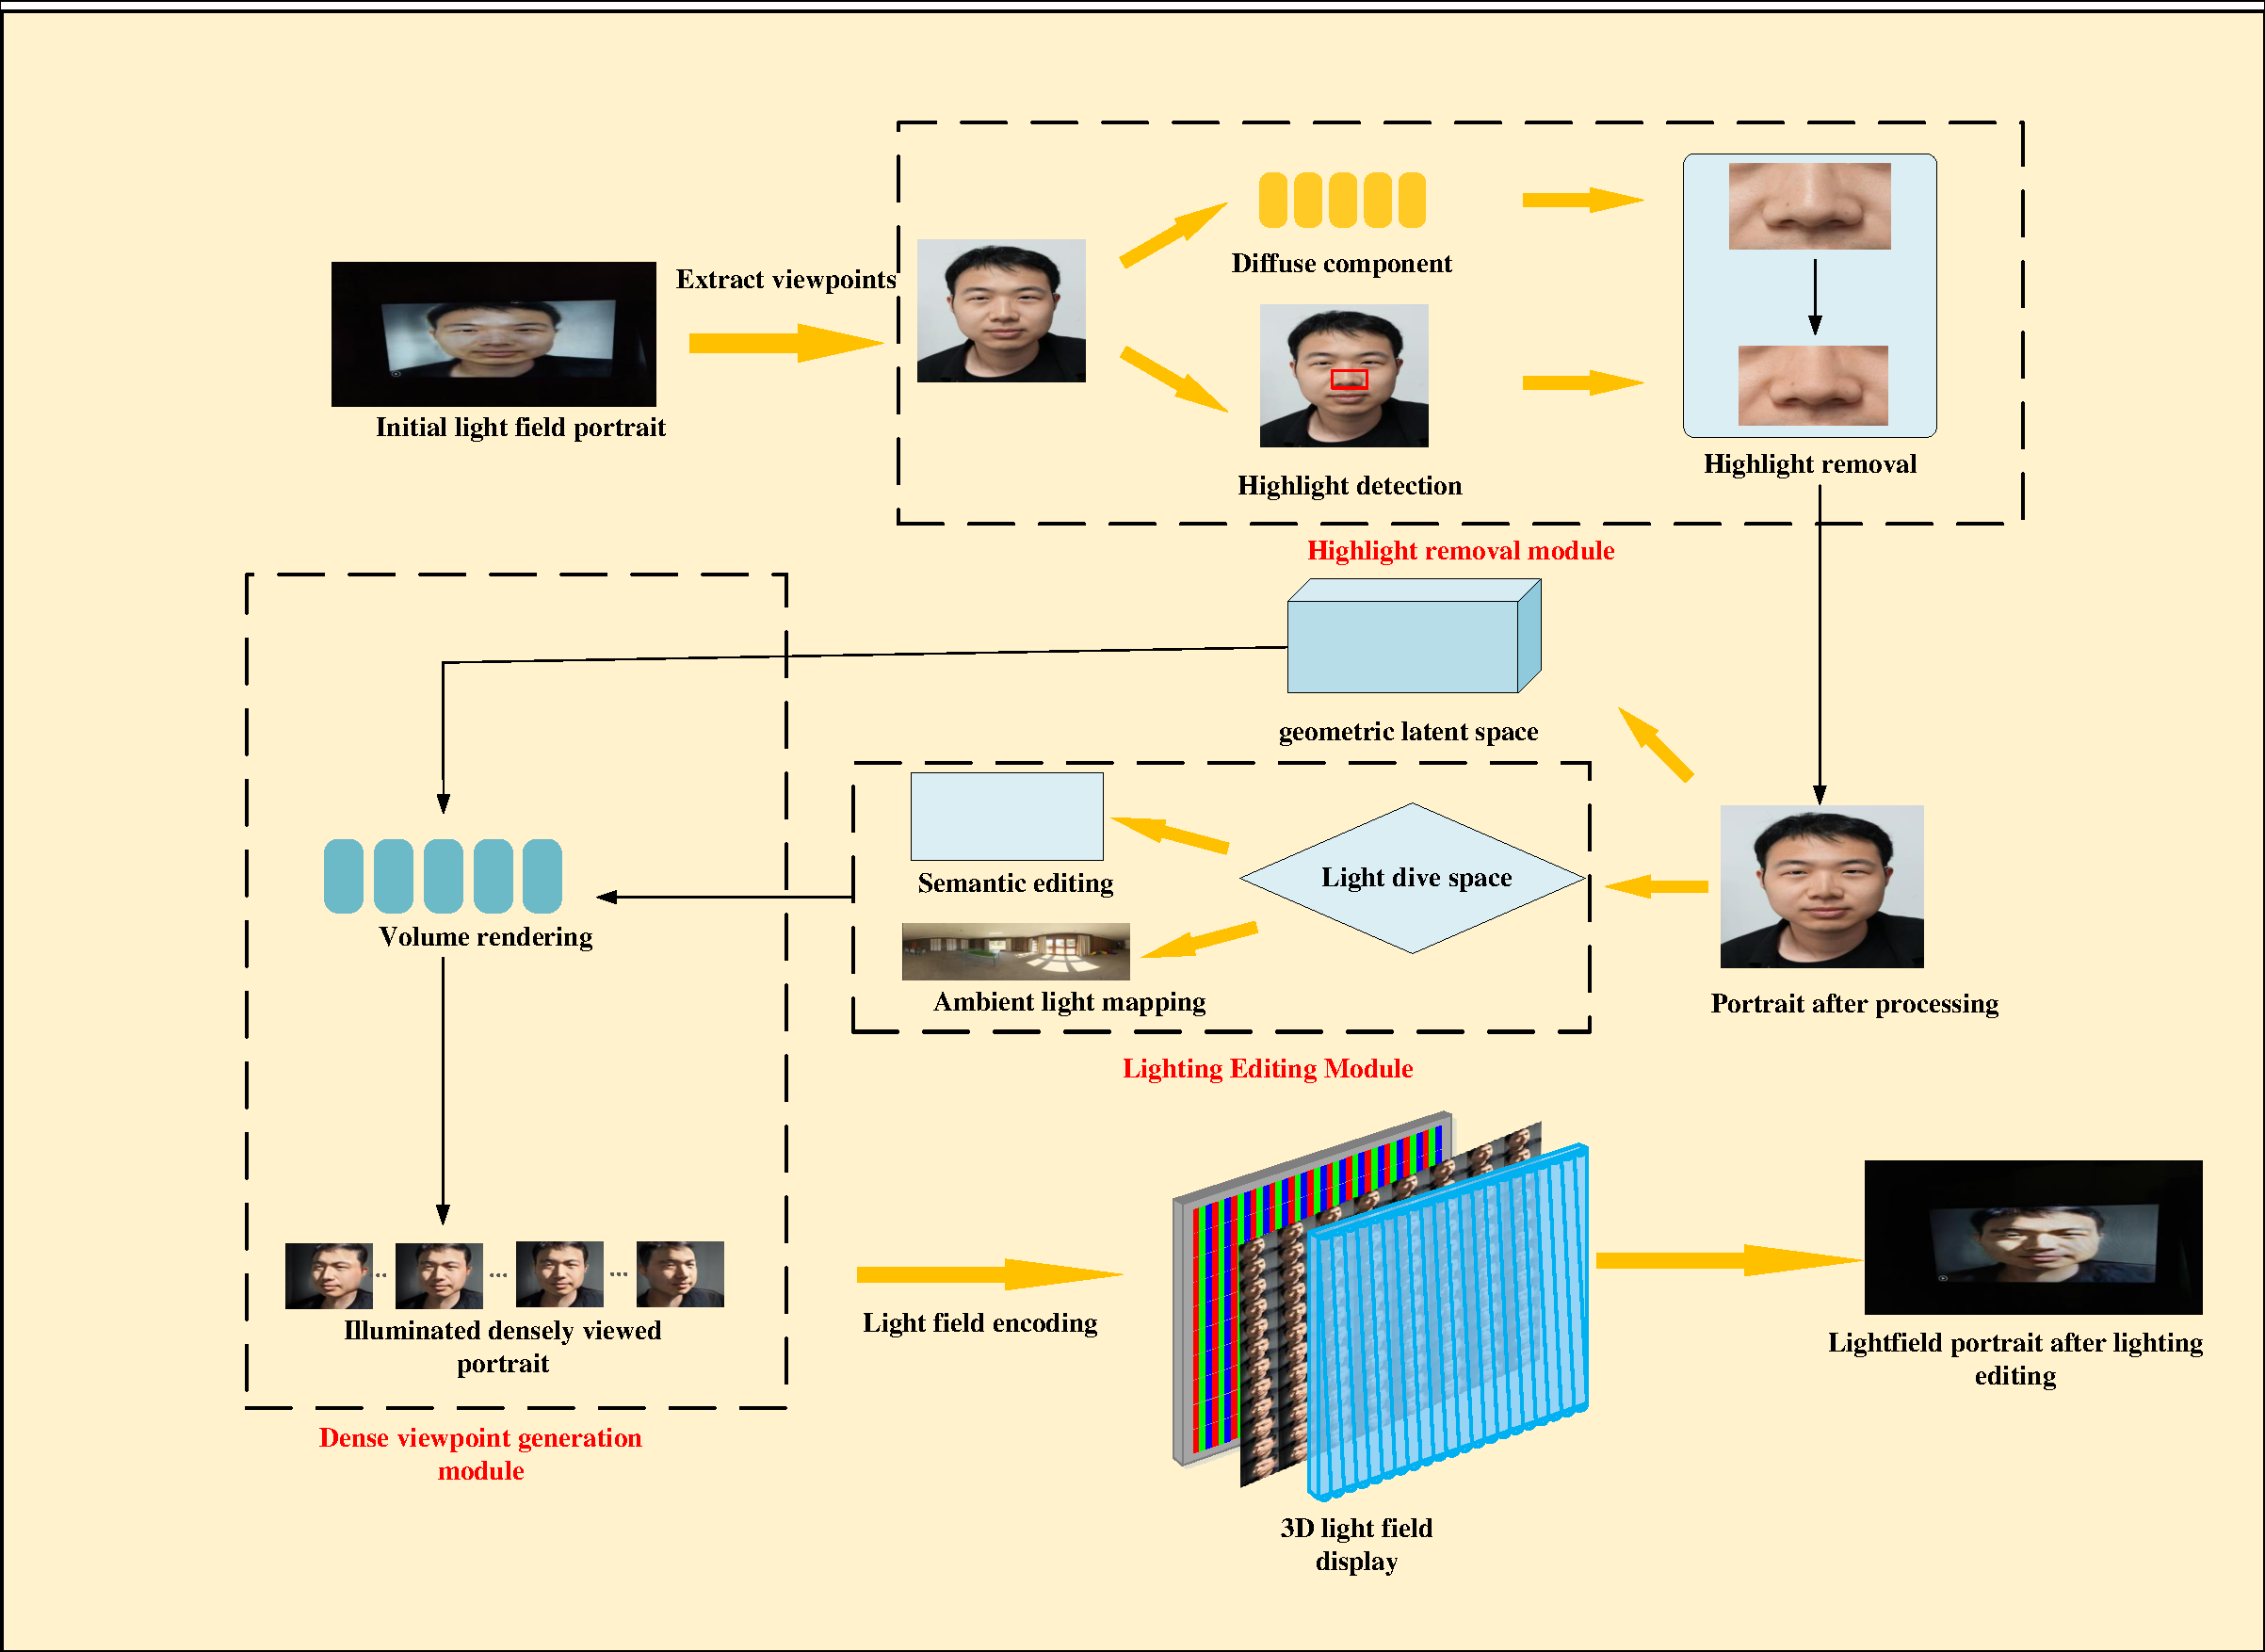
\includegraphics[width=0.8\textwidth,height=12cm]{resources/3p/3-1.pdf}
  % \bicaption{中文标题}{English Caption} % 使用中英文标题
  \caption{总体流程图} % 只使用中文标题
  \label{fig:3-1}
  %\vspace{1 cm} % 使用该指令调整上下间距
\end{figure}

具体而言，该方法由三个部分构成，分别是：高光去除模块，光照编辑模块和密集视点生成模块。

高光去除模块：针对抽取的单张人像图像，采用高光去除算法对原始光照进行预处理。 
由于人像图像的高光区域会因镜面反射导致局部亮度异常，会严重干扰后续三维重建的准确 性。该步骤旨在消除图像中高光区域对后续重建过程的干扰，结合漫反射和亮度阈值来检测 高光区域，并通过像素替换来消除高光，最后得到没有高光区域的人像图片。光照编辑模块：这一环节是实现自定义光照效果的核心所在，其通过双路径编辑策略实现任意环境光渲染与人像光照的语义化编辑。在环境光渲染路径上，运用球面调和（SH）系数计算方法，将 HDR 图像蕴含的复杂光照信息转化为 SH 系数。在人像光照语义化编辑路径上，先提取人像原始光照的 SH 系数，结合语义编辑技术，构建出可解释性强的光照属性调控模型。实现语义化的对光照方向、强度等属性的操作。通过双路径的光照编辑策略，可以满足多样化的场景需求。密集视点生成模块：基于优化后的光照关键信息，引入体渲染技术进行三维重建。输入相机参数，结合光照 SH 系数生成不同视角下的具有自定义光照效果的密集视点人像图像，最后通过光场编码后在三维光场上进行展示。

\subsection{高光去除模块}

\begin{figure}[htbp]
  \centering
  %\vspace{1 cm} % 使用该指令调整上下间距
  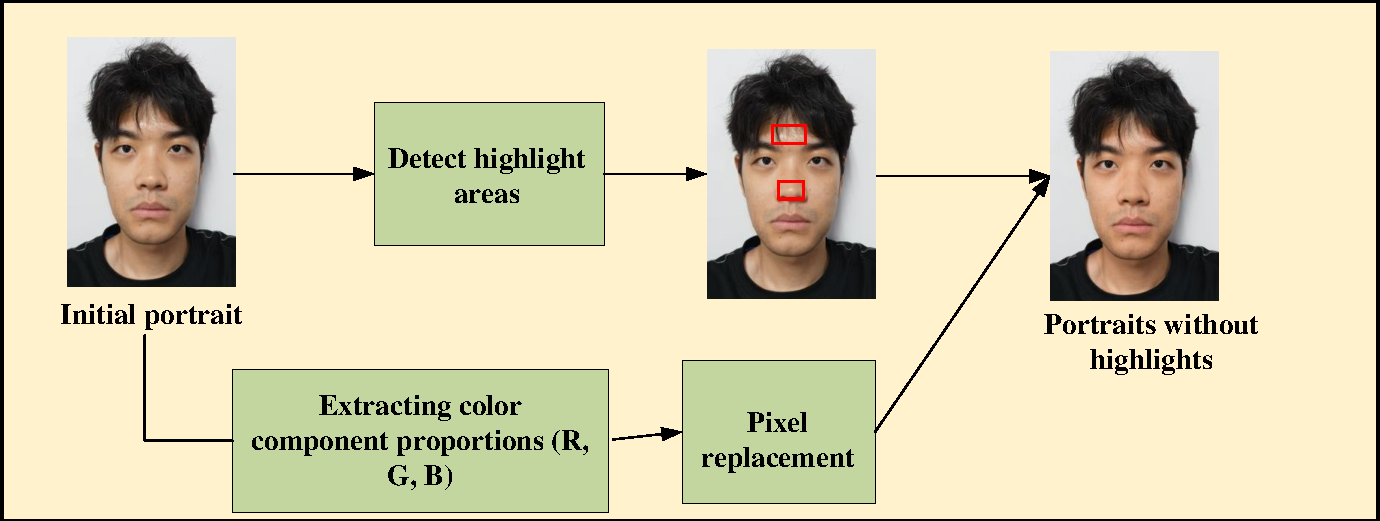
\includegraphics[width=0.8\textwidth]{resources/3p/3-2.pdf}
  % \bicaption{中文标题}{English Caption} % 使用中英文标题
  \caption{高光去除模块} % 只使用中文标题
  \label{fig:3-2}
  %\vspace{1 cm} % 使用该指令调整上下间距
\end{figure}

人像图像中，高光区域的形成源于镜面反射效应，这一现象会引发局部亮度的异常波动，进而对后续三维重建的精度产生显著干扰。为解决后续三维重建过程中的高光干扰问题，本文通过引入高光去除模块来对抽取的单张人像图像实施高光去除预处理。该模块采用高光局部去除算法对人像展开针对性处理。结合漫反射特性与亮度阈值参数构建高光区域检测机制，该双重检测机制可以精准定位图像中的高光区域，随后通过像素替换技术对已检测到的高光区域进行修正，最终输出无高光干扰的人像图像，为后续三维重建流程的顺利进行奠定基础。

高光去除模块分布两个步骤，第一步是亮度阈值检测高光区域，第二步是高光像素替换。具体流程如图\ref{fig:3-2}所示。通过检测高光区域，进行像素替换从而达到去除高光的效果。

1.	双重标准检测高光区域

本文提出一种基于双重检测标准的高光区域定位方法，通过联合亮度阈值筛选与漫反射分量偏移校验，排除了白色物体的高光误判。该设计的核心理论依据来源于双色反射模型\cite{Shafer1985}与动态亮度阈值设计\cite{蔡慧2009}。首先计算当前人像图像的三通道颜色比例，如公式\eqref{eq:2-1}所示，

\begin{equation}
\label{eq:2-1}
(r, g, b) = \left( \frac{R}{R+G+B}, \frac{G}{R+G+B}, \frac{B}{R+G+B} \right)
\end{equation}

其中，\((r, g, b)\)代表红绿蓝三通道颜色在每一个像素块儿的占比，根据双色反射模型，图像亮度可以分解为漫反射分量和镜面分量的线性叠加，其中镜面反射分量在高光区域权重显著增大。通过计算镜面反射的亮度突变特性，可能误判高亮物体（如白色陶瓷）。因此使用双重检测标准来判定高光区域。设置了高光检测的双重条件，超过了设计的阈值V并且颜色比例偏离漫反射分量会被定义为高光区域，这种双重判断标准主要是避免在处理亮度较高的图像时出现的误判问题。比如白色的杯子，亮度就超过阈值，但不是高光。对于阈值V，本文采用“均值+1.2倍标准差”的阈值策略来自适应生成阈值V，其理论依据来自于目标检测领域 ATSS 算法\cite{Zhang2020}中“均值与标准差联合决策”的思想，该方法在多个数据集上证明了对阈值自适应的有效性。具体实现是通过引入MTCNN算法\cite{Zhang2016}进行人脸区域检测与肤色样本提取，计算肤色样本中的三通道颜色的最大值 \(v_i\)，统计出 \(v_i\) 的均值 \(\mu\) 与标准差 \(\sigma\)，通过公式 \eqref{eq:2-2} 得到作为全局阈值 \(V\)：
\begin{equation}
\label{eq:2-2}
V = \mu + 1.2 \times \sigma
\end{equation}

然后由公式 \eqref{eq:brightness_threshold} 计算出人脸区域亮度阈值 \(v\)，\(v\) 代表三通道颜色中占比最大的三原色。
\begin{equation}
\label{eq:brightness_threshold}
v = \max(r, g, b)
\end{equation}

将 \(v\) 与 \(V\) 进行比较，过滤出 \(v > V\) 的像素块，最后再对这些像素块进行漫反射分量基准值校验，设置合适的偏移量 \(\delta\)，通过公式 \eqref{eq:highlight_detection} 计算出偏移量大于 \(\delta\) 的像素，即为高光区域。
\begin{equation}
\label{eq:highlight_detection}
|r - r_i| + |g - g_i| + |b - b_i| > \delta
\end{equation}

其中，\((r_i, g_i, b_i)\) 代表当前像素块所在区域在没有高光时应该具有的基准颜色比例。本文通过引入基于统计肤色模型的人脸处理\cite{Kakumanu2007} 来得到的人像基准颜色比例。

2.高光像素替换

在精准定位高光区域后，本文提出一种动态窗口自适应替换算法，通过邻域非高光像素信息重建被镜面反射污染的像素，来达到去除高光的目的。该方法的核心理论建立在局部平滑先验\cite{Buades2005}与自适应采样准则\cite{Efros1999}之上，具体流程如下：

在得到高光区域的像素块儿之后，进行像素替换即可得到去除高光后的图像。使用动态窗口进行高光替换，如公式 \eqref{eq:highlight_replacement} 所示，
\begin{equation}
\label{eq:highlight_replacement}
\begin{aligned}
R_{new} &= \frac{\sum_{(m,n)} R_{(m,n)}}{N} \\
G_{new} &= \frac{\sum_{(m,n)} G_{(m,n)}}{N} \\
B_{new} &= \frac{\sum_{(m,n)} B_{(m,n)}}{N}
\end{aligned}
\end{equation}

其中，\(R_{new}\) 代表在使用周围非高光像素的平均值替换后得到的新像素值，也就是没有高光干扰的像素。\(G_{new}\) 和 \(B_{new}\) 同理。

根据自适应采样准则来动态调整窗口大小，默认使用 \(3 \times 3\) 的窗口进行替换，计算出窗口里面的非高光区域的像素平均值，然后替换高光区域得到新的像素值。如果高光区域过大，\(3 \times 3\) 的窗口全是高光区域，则对窗口进行动态扩充到 \(5 \times 5\) 或者 \(7 \times 7\)，直到区域内有非高光像素为止，最后得到信息重建后的无高光人像。为后续光照编辑和人像重建打下基础。

\subsection{光照编辑模块}
在计算机图形学领域，精确模拟和编辑环境光照对于实现逼真的场景渲染至关重要。球面调和系数（SH）作为一种高效的光照表示方法，能够将复杂的环境光照信息紧凑地编码为一系列系数。通过计算从环境光高动态范围（HDR）图像中获取 SH 系数，从而达到使用环境光来进行重光照或者直接对光照进行编辑的效果。

1.通过环境光对人像进行重光照

根据帕塞瓦尔定理，自然光照的辐射能量主要分布于低频分量，这一特性使得9个低阶参数就足以近似在保留主要光照特征的同时，显著降低计算复杂度。为了保证重建过程不会过于复杂，又可以真实的还原光照的信息，故本文提出了一种光照编辑方法，选用了前2阶系数，一共9个SH系数来模拟光照。图\ref{fig:3-3}展示了从环境光高动态范围（HDR）图像中获取 SH 系数，进行渲染后展示在三维光场上展示的效果，由于拍摄的照片为2维的，难以表示出3D显示器所展示的立体效果，故从3个角度分别拍摄同一场景，从而得到3张图片来展示其立体效果。
\begin{figure}[htbp]
  \centering
  %\vspace{1 cm} % 使用该指令调整上下间距
  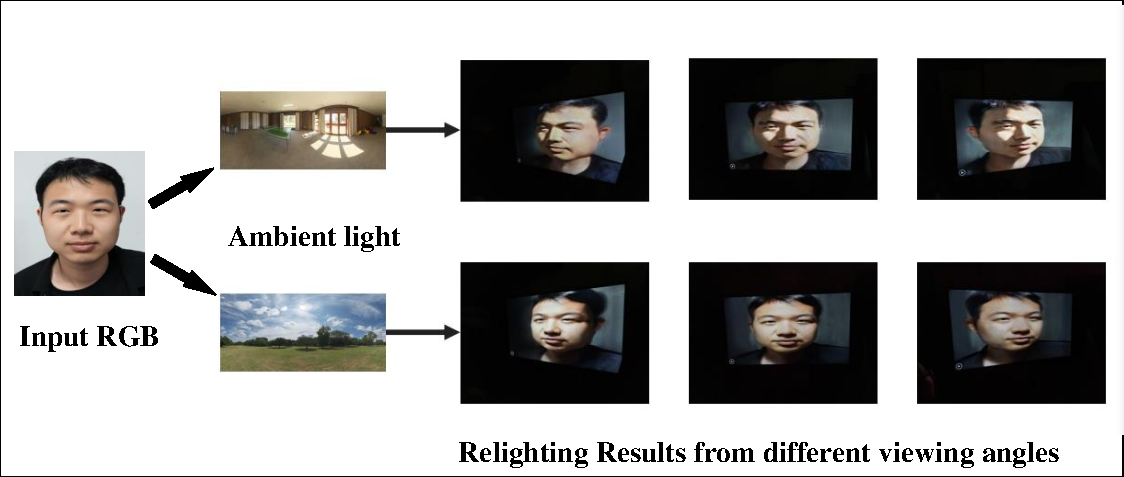
\includegraphics[width=0.8\textwidth]{resources/3p/3-3.pdf}
  % \bicaption{中文标题}{English Caption} % 使用中英文标题
  \caption{环境光重光照} % 只使用中文标题
  \label{fig:3-3}
  %\vspace{1 cm} % 使用该指令调整上下间距
\end{figure}
2.通过语义编辑人像进行光照编辑

针对环境光照的交互式编辑需求，本节提出一种面向整体亮度调节与四方向（左、右、上、下）光照控制的简易方法，通过建立自然语言语义与低阶球面调和（SH）系数的直接映射关系，实现直观高效的光照编辑。通过引入现成的自然语言处理模型BERT\cite{Devlin2019}，将用户输入的自然语言指令（例如 “增加左侧光照”“减弱顶部光源强度” 等）作为模型的输入。

该模型经过预训练已具备较强的语义理解能力，能够精准解析指令中包含的光照方向、强度变化等关键信息。模型的输出被设定为 9 个球谐函数系数，这 9 个系数可有效表征三维空间中的光照分布特性。当输入 “增加左侧光照” 这类指令时，模型会自动识别 “左侧” 对应的空间方位，并通过增大该方位所对应的 SH 系数，实现对人像左侧光照强度的针对性增强。整个实现框架如图\ref{fig:3-4}所示。首先，系统接收自然语言指令，如 “增强右侧光照”，“降低整体亮度”。随后，语义解析模块提取指令中的关键信息，明确调整方向和操作类型，系数映射模块根据预设规则，定位对应的 SH 系数并计算调整量，然后对 SH 系数矩阵进行调整。最后得到调整后的SH系数，用于后续密集视点生成模块中的使用。


\begin{figure}[htbp]
  \centering
  %\vspace{1 cm} % 使用该指令调整上下间距
  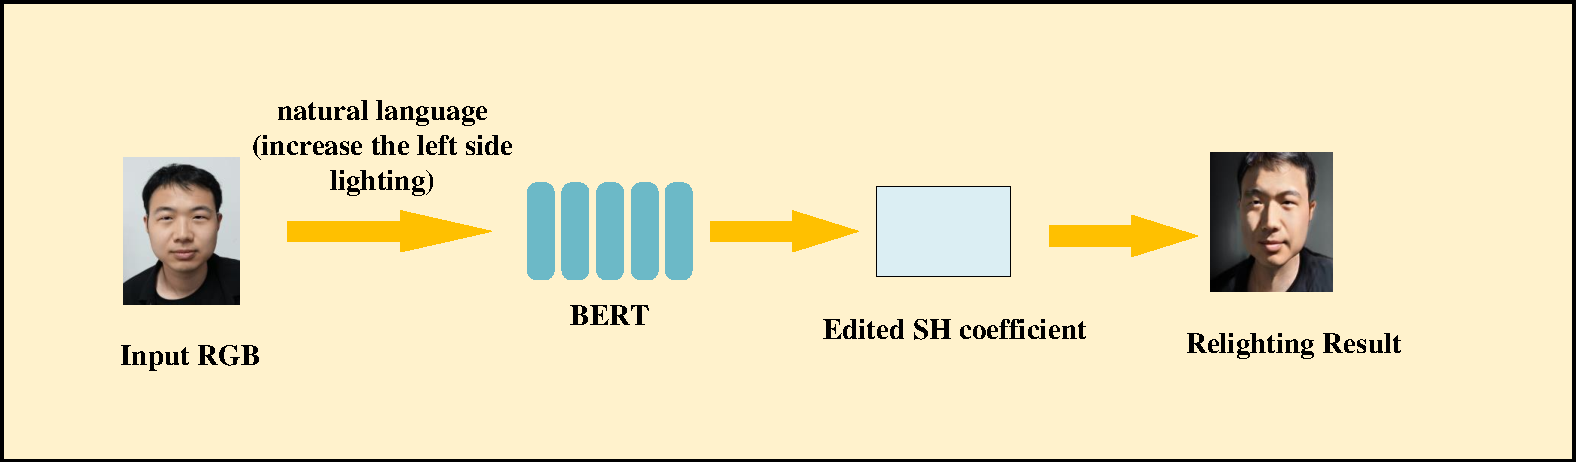
\includegraphics[width=0.8\textwidth]{resources/3p/3-4.pdf}
  % \bicaption{中文标题}{English Caption} % 使用中英文标题
  \caption{语义编辑} % 只使用中文标题
  \label{fig:3-4}
  %\vspace{1 cm} % 使用该指令调整上下间距
\end{figure}


\subsection{密集视点生成模块}
在密集视点生成模块中，将垂直视角恒定设置为 0°，在水平 ±30°的视角范围内，按照特定的采样策略均匀采集 90 个视角数据。本文引入NerfLighting框架，通过输入抽取的单张光场视差图，渲染得到模型，最后生成指定光照条件的密集人像视点。

具体来说，对于空间点 $(x, y, z)$，通过双线性插值投影到三个平面，得到特征向量如公式 \eqref{eq:f_sum} 所示：
\begin{equation}
\label{eq:f_sum}
f_{sum} = f_{xy} + f_{yz} + f_{xz}
\end{equation}

使用 MLP 解码器 $\phi$ 来预测密度 $\partial$ 和颜色特征 $a$，如公式 \eqref{eq:mlp_decoder} 所示：
\begin{equation}
\label{eq:mlp_decoder}
\phi(f_{sum}) = (\partial, a)
\end{equation}

使用阴影解码器 $\omega$ 从阴影三平面预测阴影值 $s$，如公式 \eqref{eq:shadow_decoder} 所示：
\begin{equation}
\label{eq:shadow_decoder}
s = \omega(p_{shading})
\end{equation}

得到最终颜色 $c = s \odot a$。沿相机射线积分，生成视差图，如公式 \eqref{eq:ray_integration} 所示：
\begin{equation}
\label{eq:ray_integration}
C(r) = \int_{t_n}^{t_f} T(t) \partial(r(t)) c(r(t), d) dt
\end{equation}

其中：$r$ 表示光线，$t$ 表示沿光线的采样距离，$T(t)$ 为透射率，$\partial(r(t))$ 为体密度，$c(r(t), d)$ 为辐射颜色。

为了在光场上更好的显示3D效果，本文在渲染之后根据预设的采样策略逐步生成精确的视差图。具体是基于离轴模型的视角生成方法，该方法通过调整相机内参，最终生成水平视角60度范围内的90张连续水平视差的512×512 像素的视图序列。如图\ref{fig:3-5}所示，为光场编码与裸眼 3D 显示提供了高质量输入。

\begin{figure}[htbp]
  \centering
  %\vspace{1 cm} % 使用该指令调整上下间距
  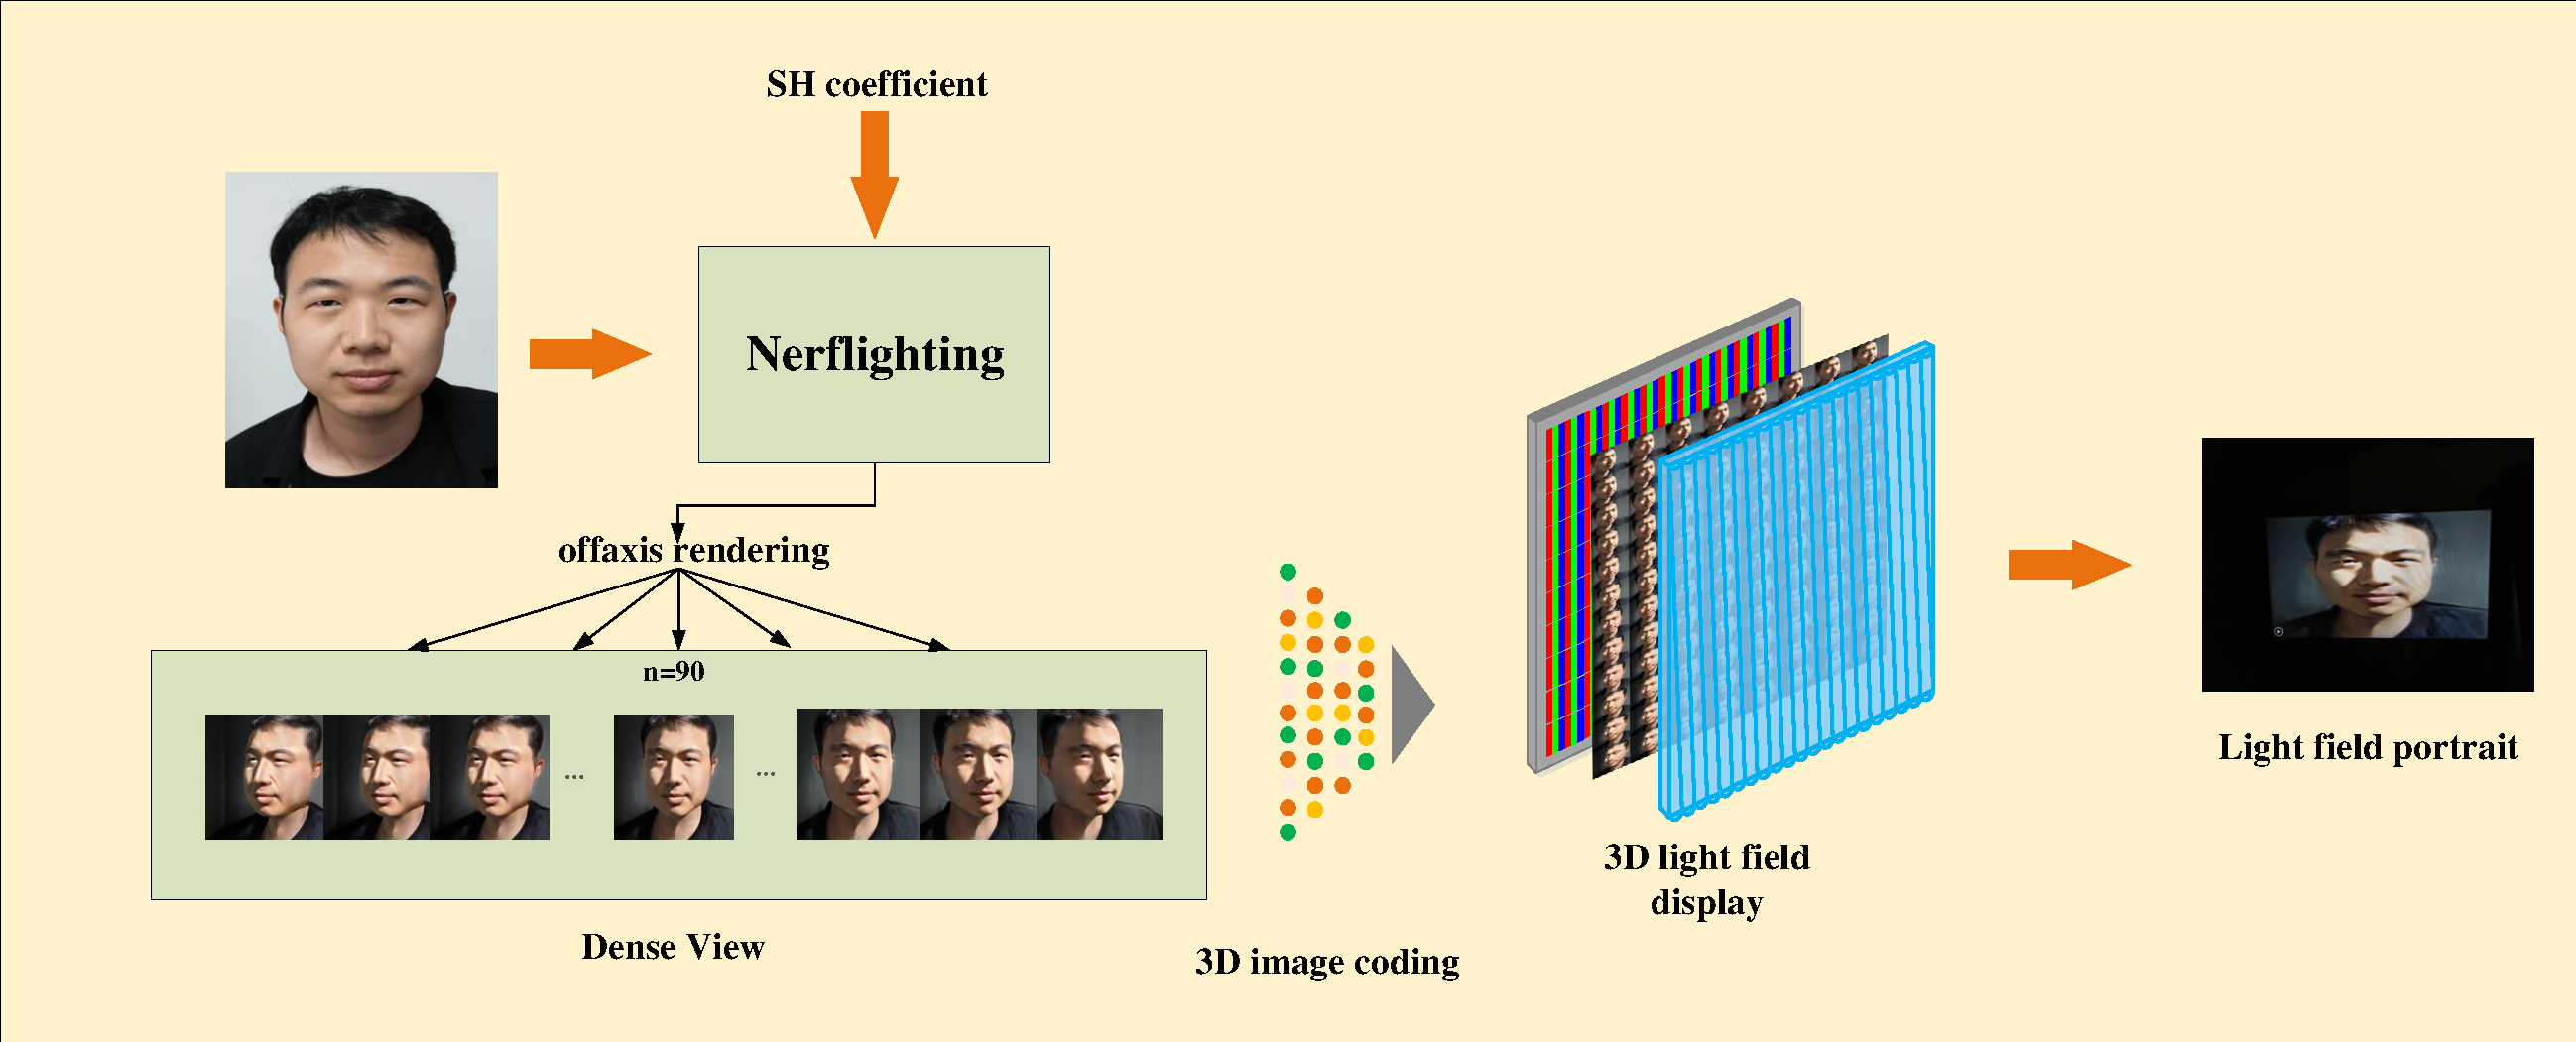
\includegraphics[width=0.8\textwidth]{resources/3p/3-5.pdf}
  % \bicaption{中文标题}{English Caption} % 使用中英文标题
  \caption{光场编码} % 只使用中文标题
  \label{fig:3-5}
  %\vspace{1 cm} % 使用该指令调整上下间距
\end{figure}

\section{实验}
在本节中，将本章提出的方法与当前先进的人像重光照方法进行了对比，并在三维光场上展示比较，进行了客观实验后证明了我们的方法在生成结果方面具有显著优势。为进一步探讨本方法的有效性，最后我们还进行了主观实验，证明了本文方法有助于显著增强3D光场带光照人像的立体感和光照一致性。
\subsection{客观实验结果及分析}
我们将本文的方法进行了定性和定量评估，并将其与如下的人像重光照方法进行了比较：NVPR\cite{Zhang2021}和LRPI\cite{Yeh2022}。

在定性评估中，我们在视觉上比较了本文方法与其他方法的结果。我们将使用本文方法，NVPR和LRPI在3种不同光照条件下生成的3D人像光场图进行了对比。
\begin{figure}[htbp]
  \centering
  %\vspace{1 cm} % 使用该指令调整上下间距
  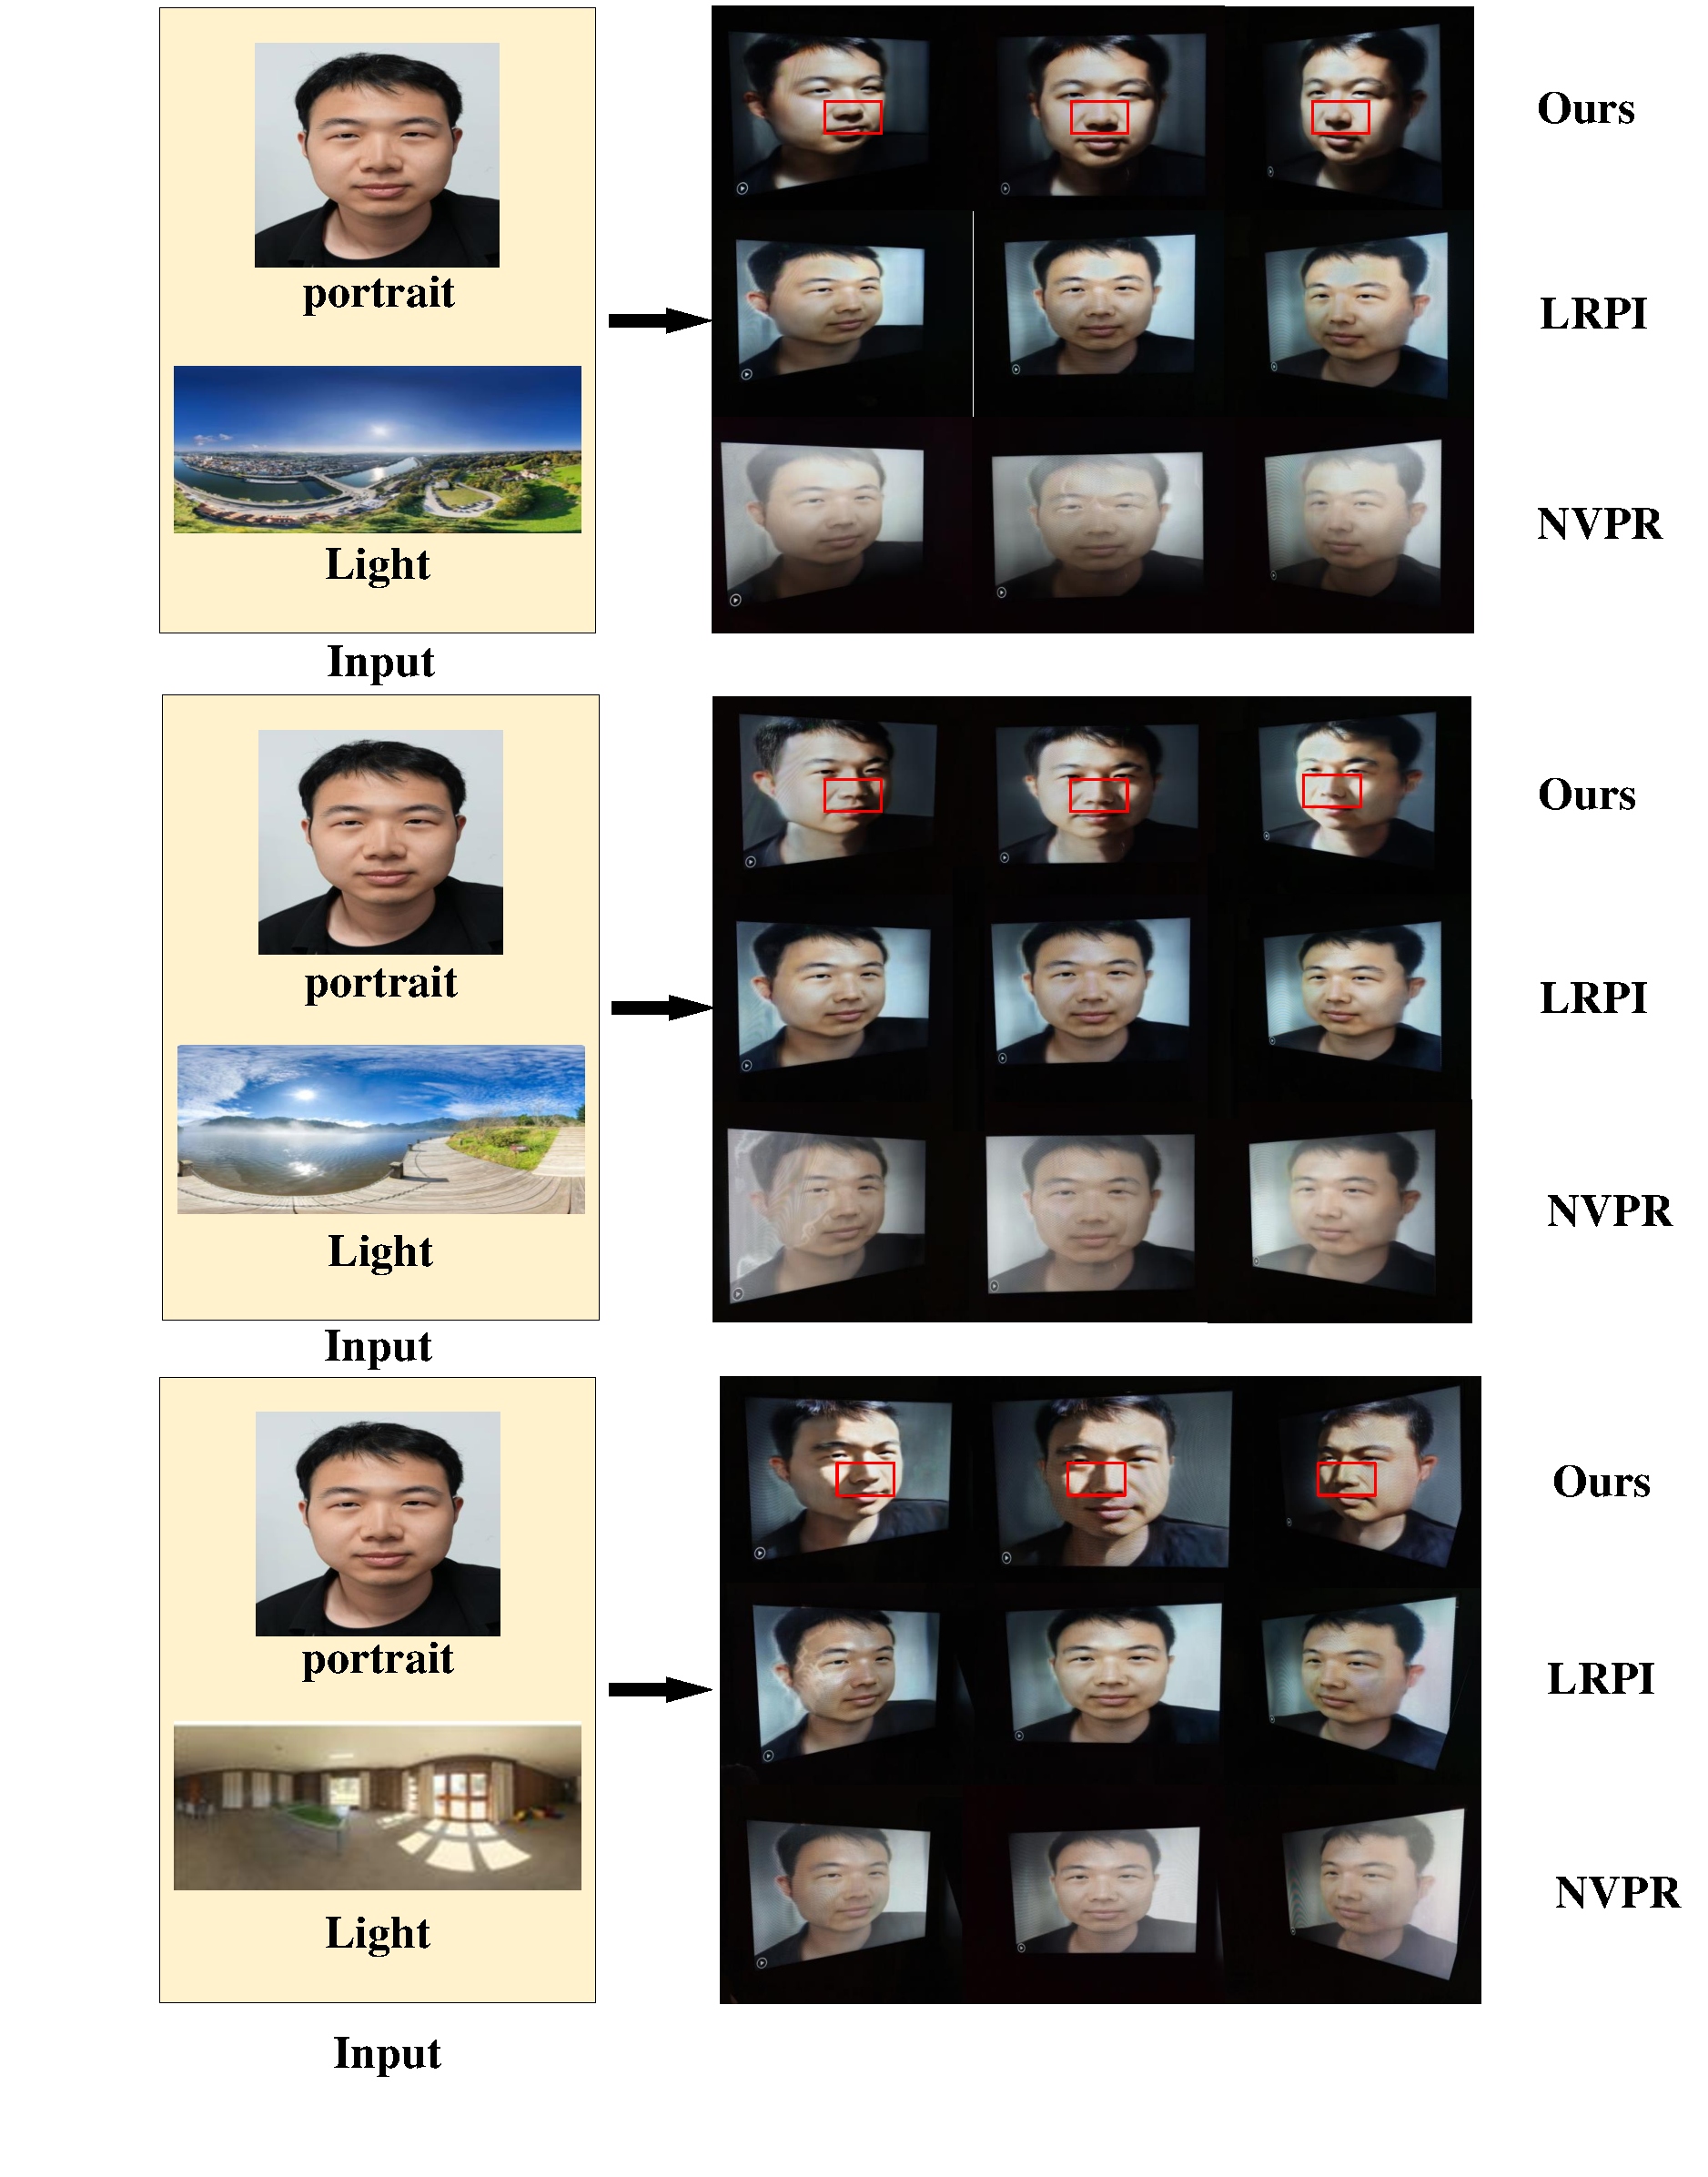
\includegraphics[width=1\textwidth]{resources/3p/3-6.pdf}
  % \bicaption{中文标题}{English Caption} % 使用中英文标题
  \caption{三种不同方法的光场人像对比图} % 只使用中文标题
  \label{fig:3-6}
  %\vspace{1 cm} % 使用该指令调整上下间距
\end{figure}

如图\ref{fig:3-6}所示。通过观察人像受光面的亮度变化是否符合实际光学原理来定性评估重光照的效果优劣。在光照直射处，人像表面应呈现高亮度且高光清晰，而处于阴影区域，亮度应显著降低，且阴影过渡自然，无生硬边界。对比 NVPR、LRPI 及本文方法，若某方法生成的人像光影在明暗分布、高光与阴影位置及形态上，与现实世界中同条件下的人像光照表现更为贴近，便表明其在视觉真实感契合度方面表现更佳。在模拟强烈太阳光下的人像重光照时，本文方法生成的人像面部受光区域亮度高且均匀，鼻梁、额头等突出部位高光精准，阴影从鼻梁、下巴等部位自然过渡，具体细节如图\ref{fig:3-6}红色区域所示。与实际生活中强光下人脸受光情况高度相似，而 NVPR 方法可能出现阴影模糊不清的问题，LRPI 方法存在高光过曝的状况。

直观上可以明显看出，与 NVPR和LRPI方法生成的3D光场图相比，我们的方法得到了更优的重光照结果。本文方法生成的人像存在明确阴影，这归因于我们引入了体渲染框架和隐式光照表示，该方法可以对人像和光照进行解耦，基于双三平面隐式表示捕捉阴影细节，并依托 3D 几何一致性与光照扰动保障阴影真实且泛化，从而呈现明确阴影，精准还原光照关键信息，从而产生更高质量的重光照人像。此外，本文与上述方法相比，本文的数据采集过程更简单、更方便。并且本文的方法具有从任意视点和光照条件下生成图像的能力，这使得本文的方法在应用于3D光场显示时具有优势。

在光场上能够生成更真实自然的光场人像之外，本文方法还可以对光照强度进行精细化的控制，以图\ref{fig:3-7}的效果为例，该方法可在保持人像身份、姿态不变的前提下，对人像右侧光照强度进行阶梯式增强：从初始的柔和侧光，到逐步提升光照能量，再到高光照强度下，整个过程中光照与阴影的过渡始终符合物理规律，无生硬断层或失真，充分验证了该方法在光照编辑上的鲁棒性和适应性。

\begin{figure}[htbp]
  \centering
  %\vspace{1 cm} % 使用该指令调整上下间距
  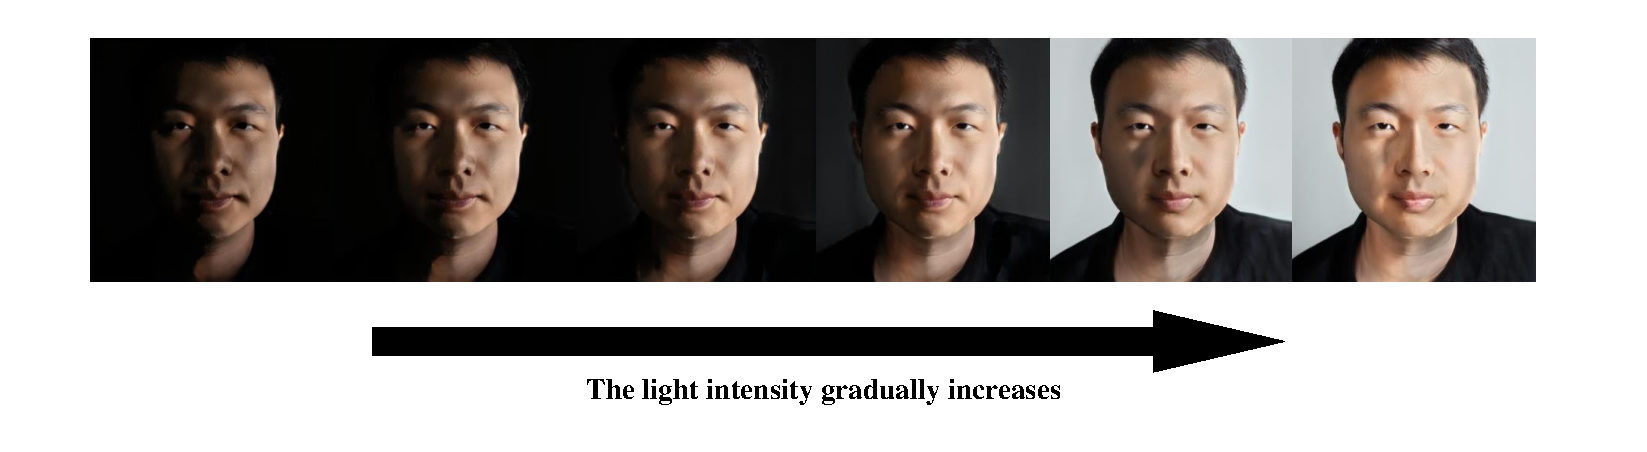
\includegraphics[width=1\textwidth]{resources/3p/3-7.pdf}
  % \bicaption{中文标题}{English Caption} % 使用中英文标题
  \caption{逐步增强人像右侧光照的对比图} % 只使用中文标题
  \label{fig:3-7}
  %\vspace{1 cm} % 使用该指令调整上下间距
\end{figure}

为了评估从输入环境图传递光照信息到重光照结果的准确性，我们从重光照图像中估计光照信息，并将其与目标光照（来自环境图的光照信息）进行比较。具体来说，我们计算了从估计 SH 系数得到的球形渲染图的平均强度，以获得一个全局标量，使其与从目标 SH 系数得到的球形渲染图的平均强度相匹配。我们通过计算重建的球形渲染图与目标球形渲染图之间的 L1 像素差异来衡量准确性。我们的结果显示出更优的数值精度，并且更接近环境图的球形渲染图。

在定量评估中，我们采用客观指标来评估方法的性能。我们使用了以下指标：

Fréchet Inception Distance(FID)：基于深度卷积神经网络特征衡量图像集之间的相似性（值越低越好）。Peak Signal-to-Noise Ratio (PSNR)：通过比较最大信号功率与噪声来指示图像保真度（值越高越好）。Structural Similarity Index (SSIM)\cite{Heusel2017}：基于感知的模型，评估亮度、对比度和结构相似性（值越高越好）。Learned Perceptual Image Patch Similarity (LPIPS)\cite{Zhang2018}：基于深度神经网络特征评估感知相似性（值越低越好）。本文的方法获得了较低的 FID 和 LPIPS 分数，以及较高的 PSNR 和 SSIM 值，表明生成图像与真实图像（Ground Truth）之间具有更高的相似性和图像质量，如表\ref{tab:3-1}所示。我们随机选择了10张图像来提取光源信息作为重光照的目标照明，其中，这10张真实图像均来自于实拍采集的人像数据。随后，我们基于此目标照明生成结果，并使用 FID、PSNR、SSIM 和 LPIPS 等指标进行比较。最后，我们计算平均值得到结果。我们的方法在这些指标上始终取得了更高的分数，表明其具有更好的重建质量且更接近真实图像。

\begin{table}[htbp]
  \centering
  \caption{同一观看视角下与前两种方法的指标对比}
  \label{tab:3-1}
  \small
  \begin{tabular}{lccccc}
    \toprule
    Method & Lighting $\downarrow$ & FID $\downarrow$ & PSNR $\uparrow$ & SSIM $\uparrow$ & LPIPS $\downarrow$ \\
    \midrule
    NVPR  & -                    & 36.54           & 28.66           & 0.6288          & 0.30             \\
    LRPI  & 0.0654               & 36.15           & 28.44           & 0.8145          & 0.23             \\
    Ours  & 0.0607               & 33.55           & 32.06           & 0.8954          & 0.19             \\
    \bottomrule
  \end{tabular}
\end{table}

我们还测试了该方法光照编辑的推理时间，在单块 NVIDIA RTX 3090 GPU 上，对1K分辨率的静态人脸进行光照编辑的平均耗时如下表所示：

\begin{table}[htbp]
  \centering
  \caption{光照编辑单帧推理时间对比}
  \label{tab:inference_time_3090}
  \begin{tabular}{lccc}
    \toprule
    Method & NVPR    & LRPI    & Ours     \\
    \midrule
    Time(s) $\downarrow$ & 230.45  & 180.21  & 25.92    \\
    \bottomrule
  \end{tabular}
\end{table}

实验结果表明，本文方法在保持更高重建质量和更接近真实图像视觉效果的同时，光照编辑效率也得到了显著提升。

\subsection{主观实验结果及分析}

为进一步探讨本方法的有效性。本文基于三维光场显示器对实验结果进行了主观实验，来对三维光场人像光照编辑的结果进行评价。实验主要分为两个部分，将本文方法编辑得到的三维光场人像和单视图编辑得到的三维光场人像进行对比，主要评估不同光照条件下光场人像的真实度和不同视角下光照一致性的情况。

实验选用了单视图单张依次编辑三维光场人像光照的方法与本方法进行对比，实验分别在三个不同人像的基础上，编辑了包含左侧光照，顶部光照，右侧光照，底部光照四种不同的光照场景，总共是24组三维光场人像场景，编辑好后，进行光场编码，并在三维显示器上进行显示，其中方法A代表本文的方法，方法B代表单视图单张依次编辑三维光场人像光照的方法，主观实验中方法A和方法B生成的部分3D光场人像如图\ref{fig:3-8}所示，其中左侧的图像均来自于实拍采集的人像数据。右侧分别是使用方法A生成的部分三维光场人像场景和使用方法B生成的部分三维光场人像场景。

24组场景，编号为1到24。比如第一组场景里面的使用本文的方法编辑生成的三维光场人像就用1(a)表示。实验参与者进行观看评估。主观实验的参与者中，男性10名，女性10名，视力正常或矫正后正常，无色彩感知障碍，所有参与者都给予了书面知情同意。

\begin{figure}[htbp]
  \centering
  %\vspace{1 cm} % 使用该指令调整上下间距
  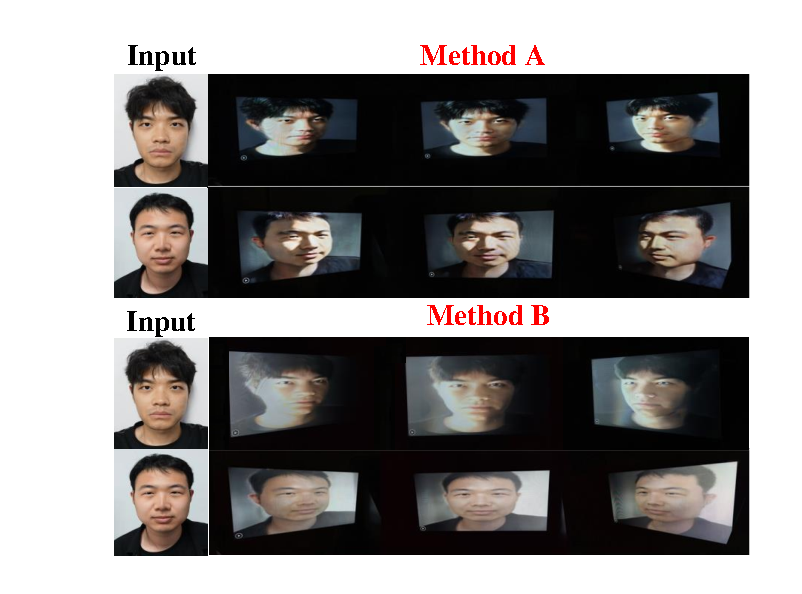
\includegraphics[width=1\textwidth]{resources/3p/3-8.pdf}
  % \bicaption{中文标题}{English Caption} % 使用中英文标题
  \caption{主观实验中方法A和方法B生成的部分3D光场人像} % 只使用中文标题
  \label{fig:3-8}
  %\vspace{1 cm} % 使用该指令调整上下间距
\end{figure}

在主观实验流程中，实验流程如下，实验会将会对24组场景在三维显示器上展示，每一组场景有2个场景，参与者对每一组的两个场景有1分钟时间左右观察，观察后对三维光场人像添加了光照之后的真实感和光照一致性进行评估，比如，第一组我们会依次展示场景1(a)，1(b)两个A，B方法生成相同光照条件的场景。参与者对于每一组场景进行投票，将票投给主观感受上更具有立体感的方法。光照一致性的投票如上，每一个场景最多可以获得20张选票。依次播放完24组场景，整个实验流程大约耗时20分钟。

实验场地如图\ref{fig:3-9}所示，我们使用裸眼3D显示器，参数如表\ref{tab:3-2}所示。

\begin{table}[htbp]
  \centering
  \caption{3D光场的显示参数}
  \label{tab:3-2}
  \small
  \begin{tabular}{lc}
    \toprule
    Display Parameters & Value \\
    \midrule
    Single view resolution & $960 \times 540$ \\
    ColNum & 8 \\
    RowNum & 12 \\
    View number & 96 \\
    Inclined angle & $8.5308^\circ$ \\
    LineNum & 28.08119 \\
    Angle of view & $100^\circ$ \\
    \bottomrule
  \end{tabular}
\end{table}

\begin{figure}[htbp]
  \centering
  %\vspace{1 cm} % 使用该指令调整上下间距
  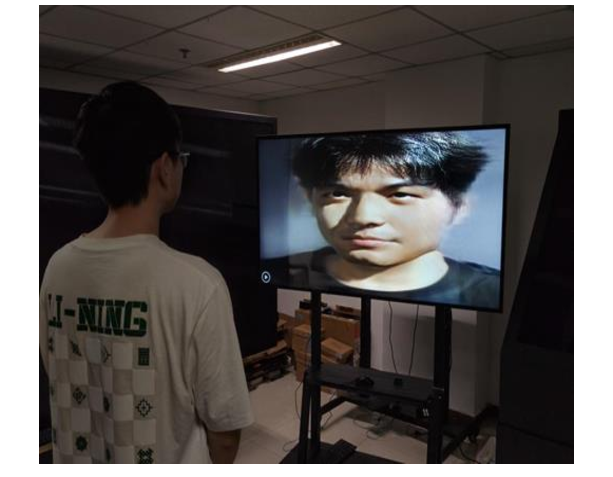
\includegraphics[width=1\textwidth]{resources/3p/3-9.pdf}
  % \bicaption{中文标题}{English Caption} % 使用中英文标题
  \caption{实验场地} % 只使用中文标题
  \label{fig:3-9}
  %\vspace{1 cm} % 使用该指令调整上下间距
\end{figure}

参与者站在距离显示器2米左右位置上进行观察，因为需要观察三维显示器不同视角下的光照一致性情况，参与者在观察时会进行左右的来回走动观察和感受。观察结束后再进行投票，投完票之后再进行下一个场景的观察与投票。为了避免每一组的AB场景会对后续场景的评估产生影响，实验会保证每一组的AB场景的播放顺序是随机的，并且参与者可以反复观看进行对比，同时也减少了惯性思维对实验结果的影响。

为了方便对比，本文提出的方法用后缀A进行表示，单视图依次编辑光照的方法用后缀B表示。通过主观实验对三维光场人像的展示，主要做两个部分的实验，分别是不同参与者对24组场景的立体感的评价结果和不同参与者对24组场景的光照一致性的评价结果。
\begin{figure}[htbp]
  \centering
  %\vspace{1 cm} % 使用该指令调整上下间距
  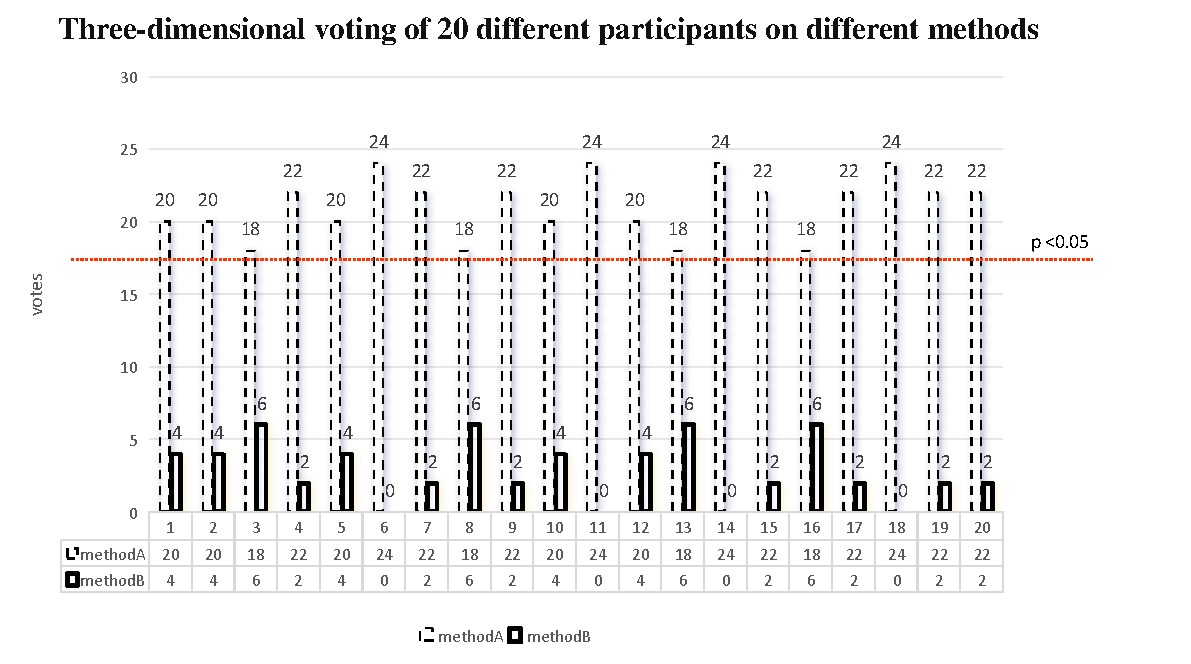
\includegraphics[width=1\textwidth]{resources/3p/3-10.pdf}
  % \bicaption{中文标题}{English Caption} % 使用中英文标题
  \caption{20个不同参与者对不同方法的立体感投票情况} % 只使用中文标题
  \label{fig:3-10}
  %\vspace{1 cm} % 使用该指令调整上下间距
\end{figure}
% \subsubsection{三级标题}

3D立体感的评价结果如图\ref{fig:3-10}所示。假设参与者的投票遵循二项分布 ，对每个场景都应用了二项检验。如果两种方法编辑人像光照后给参与者产生的立体感类似，则投票数预计为总票数中的 1/2。因此，如果某种方法的得票数明显大于此值，说明该方法能够给呈现出更好的3D立体感。

对于图\ref{fig:3-10}所示的结果展示，柱状图统计了所有20名参与者参加24次实验的投票结果汇总，其中，虚线柱代表方法A（本文方法）编辑光照得到的选票数，实线柱代表方法B（单张视图依次编辑三维光场人像）编辑光照得到的选票数，方法A在的3D立体感上的最低得票率为80\%，最高得票率为100\%，平均得票率为88.75\%。假设方法A和方法B对参与者呈现的3D视觉立体感类似，在统计意义上的显著的的得票率为20票（n=24 的二项检验，多次比较的 Bonferroni校正\cite{Bonferroni1936}P<0. 05），获得超过20票，在图10中已经划线表示，即可否定原假设，认为票数更多的方法能够呈现更好的3D立体感，在20名参与者中，有16名参与者认为方法A编辑后的到的三维光场人像的3D立体感更佳。
\begin{figure}[H]
  \centering
  %\vspace{1 cm} % 使用该指令调整上下间距
  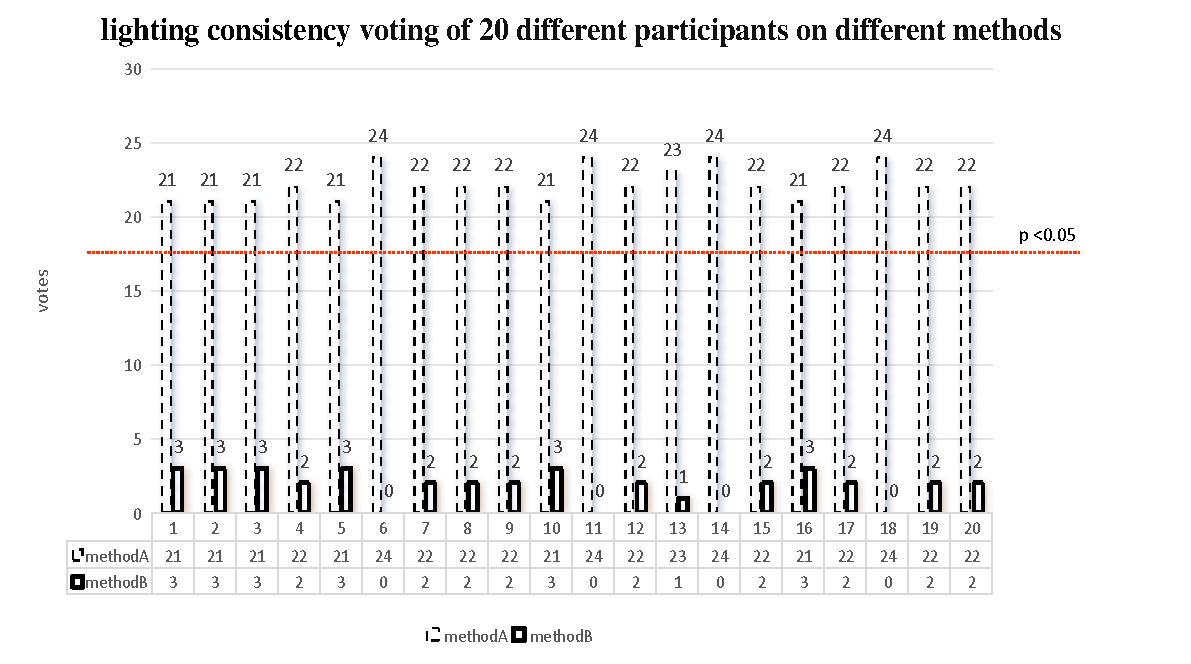
\includegraphics[width=1\textwidth]{resources/3p/3-11.pdf}
  % \bicaption{中文标题}{English Caption} % 使用中英文标题
  \caption{20个不同参与者对不同方法的光照一致性投票情况} % 只使用中文标题
  \label{fig:3-11}
  %\vspace{1 cm} % 使用该指令调整上下间距
\end{figure}

光照一致性的评价结果如图\ref{fig:3-11}所示。参与者在指导下通过左右移动观察3D显示器展示的内容，然后根据主观感受来投票选出不同视角下光照一致性更强的场景。假设参与者的投票遵循二项分布 ，对每个场景都应用了二项检验。如果两种方法编辑人像光照后给参与者产生的光照一致性类似，则投票数预计为总票数中的 1/2。因此，如果某种方法的得票数明显大于此值，说明该方法能够给呈现出更好的光照一致性。

对于图\ref{fig:3-11}所示的结果展示，柱状图统计了所有20名参与者参加24次实验的投票结果汇总，其中，虚线柱代表方法A（本文方法）编辑光照得到的选票数，实线柱代表方法B（单张试图依次编辑三维光场人像）编辑光照得到的选票数，方法A在的3D立体感上的最低得票率为80\%，最高得票率为100\%，平均得票率为92.29\%。假设方法A和方法B对参与者呈现的光照一致性类似，在统计意义上的显著的的得票率为20票（n=24 的二项检验，多次比较的 Bonferroni校正P<0. 05），获得超过20票，在图11中已经划线表示，即可否定原假设，认为票数更多的方法能够呈现更好的光照一致性，在20名参与者中，所有参与者认为方法A编辑后的到的三维光场人像的光照一致性更佳。
\begin{table}[htbp]
  \centering
  \caption{实验方法得票总数}
  \label{tab:3-3}
  \small
  \begin{tabular}{lc}
    \toprule
    Type of experiment & Total votes \\
    \midrule
    three-dimensional (method A) & 428 \\
    three-dimensional (method B) & 52 \\
    lighting consistency (method A) & 443 \\
    lighting consistency (method B) & 37 \\
    \bottomrule
  \end{tabular}
\end{table}

对于表\ref{tab:3-3}的统计结果，记录了在24组不同场景的20名参与者分别进行两组实验的投票结果汇总。分别是光照一致性实验和立体感实验，方法A(本文的方法),方法B(基于单视图编辑光照的方法)。得票数为这两种方法编辑在这24组场景的背景下，分别从20名参与者身上得到的选票数。统计得到方法A在24组场景下的立体感得票率为89.19\%，方法B的平均得票率为10.81\%。假设方法A编辑三维光场人像光照后的立体感没有提升，那统计结果三种方法的得票率应在50\%上下浮动。证明了使用本文方法编辑光场人像光照后，立体感和光照一致性均得到了提升。

\section{本章小结}
本章提出了一种关键信息驱动的三维光场人像光照的编辑方法，该方法通过抽取多视图，通过获取漫反射分量，并结合高光阈值多重判断来去除图像高光，因为三维光场现实内容由多张视差图构成，并且视差图光照不均匀或者存在高光，高光会贴合在人像上，对后续重建效果产生影响，所以先进行光照均匀化处理。然后进行重建，将图像解耦成几何空间和光照潜空间，通过全景 HDR 图像快速获取环境光信息并通过语义级别描述的对光照潜空间的关键信息进行编辑，结合几何空间和光照潜空间，并通过体渲染渲染得到密集视差图，最后在3D显示器上进行显示验证，完成对三维光场人像光照的编辑。

本章进行了客观实验和主观实验，在客观实验中，与当前重光照方法NVPR和LRPI进行了对比，本方法可以生成更自然真实的光照条件，没有出现光线泛白，不同角度光线不一致的问题，在FID、PSNR、SSIM 和 LPIPS 等指标中都取得了更优的分数，并且能够更快的进行静态人像光照编辑。在主观实验中，本文方法和依次对多张视差图进行人像光照的编辑方法进行了实验对比。在立体感上，本方法得票率为89.19 \%，证明了本方法编辑后的人像具有更高的立体感，在光照一致性的投票上，本方法得票率为92.29\%，证明了本方法编辑后的人像具有更好的光照一致性。上述实验证明了该方法在提高了光照一致性的前提下，简单高效的实现对三维光场光照的编辑。本方法还可以通过环境光照来编辑光场人像的光照，并取得了较好效果，并且可以显著增强3D光场带光照人像的立体感和光照一致性，可能成为未来对静态场景3D光场显示进行光照编辑的重要方法。

目前研究工作中仍有不少可改进之处。在拓展至动态人脸视频场景时仍存在明显局限性：面对人脸的连续姿态变化、表情运动，现有框架难以兼顾帧间光照的时序连续性，易出现光照闪烁、高光跳变等问题；同时，多视角光照一致性的约束仅针对单帧静态几何，无法适配动态场景下的跨帧几何形变，导致动态序列的多视角光照出现时空失配。针对上述动态场景的技术痛点，后续工作将聚焦于时间 - 空间双维联合优化，构建专门面向动态人脸的三维光场光照编辑框架，重点解决时序闪烁与动态多视角光照失配问题，实现高质量的动态三维光场人脸光照编辑。


%第三章
\include{Chapter/chapter04}%第四章
\chapter{总结与展望}
本文围绕三维光场人脸光照编辑这一核心课题，针对静态与动态场景下的技术痛点，构建了从基础方法到优化框架的完整技术体系，通过理论创新与实验验证，有效解决了现有方法中存在的采集设备复杂、多视角一致性不足、动态时序闪烁等关键问题，主要研究成果与核心内容如下。
\section{研究内容与创新}
提出了一种关键信息驱动的三维光场静态人脸光照编辑方法。针对静态三维光场人像光照编辑中 “多视图独立编辑导致一致性差” 与 “密集采集设备成本高昂” 的双重痛点，提出了关键信息驱动的光照编辑方法，核心创新与成果如下：构建了 “高光去除 - 光照编辑 - 密集视点生成” 三级框架：通过双重检测标准（亮度阈值 + 漫反射分量校验）精准定位高光区域，结合动态窗口自适应替换算法消除高光干扰，为后续光照编辑提供干净的输入基础；采用双路径光照编辑策略，既支持从 HDR 图像提取 SH 系数实现环境光重光照，又能通过 BERT 模型解析自然语言指令，实现光照方向、强度的语义化调控；基于 NeRF 体渲染框架，生成水平 ±30° 范围内 90 个视角的密集视差图，满足光场显示需求。

实验验证成效显著：客观实验中，与 NVPR、LRPI 等主流方法相比，本文方法在 FID（33.55 vs 36.54/36.15）、PSNR（32.06 vs 28.66/28.44）、SSIM（0.8954 vs 0.6288/0.8145）及 LPIPS（0.19 vs 0.30/0.23）等指标上均实现最优，光照误差（LE=0.0607）低于对比方法；单帧推理效率大幅提升，在 RTX 3090 GPU 上处理 1K 分辨率图像仅需 25.92s，远快于 NVPR（230.45s）与 LRPI（180.21s）；主观实验中，在三维光场显示器上的立体感知得票率达 89.19\%，多视角光照一致性得票率 92.29\%，显著优于单视图逐帧编辑方法，证明该方法在保证光照一致性的前提下，实现了简单高效的静态光场人像光照编辑。


提出了一种空间双维联合优化的动态光照编辑框架针。对静态方法扩展至视频序列时出现的时序闪烁与多视角光照失配问题，提出动态光照一致性优化框架，核心创新与成果如下：
时序一致性优化模块：采用共享编码器提取相邻帧稳定语义特征，通过光流估计网络实现跨帧空间对齐，将时间一致性问题转化为空间对齐问题；设计光照分量提取网络解耦几何与光照特征，仅对光照响应分量施加 “特征 L1 + 像素残差 L2” 双重损失约束，在抑制帧间闪烁的同时保留表情与姿态的自然动态。实验表明，该模块使时序稳定性指标 WE 降至 0.0004，帧间 LPIPS 低至 0.1912，显著优于 SMFR（WE=0.0022）与 E4E（帧间 LPIPS=0.2344）。
多视角一致性优化模块：基于相机内外参构建投影矩阵，结合 NeRF 获得统一三维几何模型，通过三维表面采样将多视角光照约束转化为三维点光照观测问题；引入多因子加权聚合机制（可见性 + 法线夹角 + 光照置信度），实现可靠的光照统一估计，再通过一致性回投影优化还原至二维视角。该模块使多视角光照误差 LE 降至 0.7922，光照不一致度 LI 达 0.2644，均优于对比方法。

综合性能验证：客观实验中，本文方法在 FID（33.5501）、PSNR（32.0226）等生成质量指标上保持领先，身份一致性 ID 达 0.5122，优于对比方法；主观实验中，动态光照连续性、多视角一致性及整体三维沉浸感综合评分达 4.73，较 PTI 方法（3.08）提升 53.57；消融实验验证了时序一致性模块儿的重要性。

\section{未来与展望}
本文虽在三维光场人脸光照编辑领域取得了阶段性成果，但仍存在可拓展与优化的方向，结合技术发展趋势与实际应用需求，未来研究可聚焦以下方面：

场景通用性拓展：当前方法主要针对人像场景设计，后续可研究非人像场景（如工业零件、自然景物）的几何与光照解耦方法，通过优化三维重建与光照估计策略，提升算法对复杂轮廓、多样材质的适应性，拓宽技术的应用场景。

实时性优化与硬件适配：现有方法在处理高分辨率视频时，实时推理性能仍有提升空间。未来可通过模型轻量化（如剪枝、量化、蒸馏）、硬件加速（如 GPU/TPU 专用算子优化）及算法简化（如高效光流估计、稀疏采样策略），降低计算复杂度，实现高清三维光场视频的实时光照编辑，满足直播、AR/VR 等实时交互场景的需求。

生成式 AI 融合与精细编辑：结合生成式对抗网络（GAN）、扩散模型等先进生成式 AI 技术，实现更精细的光照细节编辑（如局部光斑调控、纹理光影交互）；探索多模态输入（文本、语音、草图）的光照编辑方式，进一步降低用户操作门槛，提升交互灵活性与编辑自由度。

多场景光照交互与动态适配：当前方法主要针对固定光照编辑需求，未来可研究动态场景下的光照自适应调整策略，实现光照与场景运动（如人脸大幅度动作、视角剧烈切换）的实时适配；探索多物体光场场景中的光照交互机制，支持不同物体间的光照反射、阴影投射等物理效果模拟，提升光场显示的整体真实感与沉浸感。

%第五章



\bibliographystyle{gbt7714-numerical}
{\zihao{5}
\bibliography{Bib/thesis} % 参考文献
}

\backmatter
\include{Chapter/Chapter_abbreviation} % 缩写附录
\ifWithOptionBlind \else
\begin{acknowledgement}
时光荏苒，求学至今，离不开许多师长与亲友的关心、支持与帮助。在此谨向所有帮助过我的人致以最诚挚的谢意。

首先，衷心感谢我的导师桑新柱老师。感谢您在课题研究与论文撰写过程中给予我的悉心指导与耐心帮助，您的严谨治学态度和认真负责的工作作风使我受益匪浅。

同时，感谢于迅博老师在学习和科研过程中给予我的指导与鼓励。

感谢李宁驰师兄、聂子涵师姐在课题推进过程中提供的经验分享与具体帮助，让我在遇到困难时能够及时获得启发和支持。

感谢石恒、孙鑫宇、杨博中、祝子豪、陈鑫源在论文研究过程中对实验数据的提供与支持，你们的帮助为本文工作的顺利开展提供了重要保障。

感谢我的舍友们在生活中的陪伴、理解与包容，你们让平凡的学习生活充满温暖。

最后，特别感谢我的父母。感谢你们一直以来无私的付出、坚定的支持与默默的守护，是你们给予我不断前行的勇气与力量。
\end{acknowledgement}
 % 致谢
\fi
\begin{publication}
\definecolor{Maroon}{HTML}{701112}
\newcommand{\IF}[1]{\textcolor{Maroon}{IF = #1}}
本人攻读学位期间共发表论文X篇，其中，第一作者X篇，学生一作X篇，第二作者X篇，其他参与论文共X篇：
本人攻读学位期间取得如下创新成果：发表论文1篇，发明专利3项。
\begin{enumerate}
\item 杨垚杰, 于迅博, 高鑫, 等. 关键信息驱动的三维光场人像光照的编辑方法[J/OL]. 光学学报, 1-24[2026-03-04]. https://link.cnki.net/urlid/31.1252.O4.20260124.1323.002.
\end{enumerate}

发明专利3项：
\begin{enumerate}
\item 北京邮电大学深圳研究院. 一种三维场景显示方法、系统、设备及介质: 202411832954.9[P]. 2025-04-04.
\item 北京邮电大学. 立体显示器显示深度的测量方法、装置、设备及介质: 202311628090.4[P]. 2024-03-22.
\item 北京邮电大学. 立体显示器深度的测量方法、装置、设备和存储介质: 202311532440.7[P]. 2024-03-08.
\end{enumerate}


\end{publication}
 % 创新成果
\ifWithOptionBlind \else
\include{Chapter/Chapter_experience} % 作者学习经历
\fi

\end{document}
